\chapter{Results} \label{sec:Res}

\section{Review Feature Prediction} \label{sec:Res_RF}

In this section, the predictive validity of the models that were trained to predict different review features will be evaluated, compared and discussed.

\subsection{Polarity} \label{sec:Res_RF_Pol}

The overall accuracy of all of the models that were trained to predict review polarities will first be compared. Then, detailed classification results for the BERT classifiers; the best performing non-BERT classifiers, eg SGD or LSVC; and the best performing baseline classifiers will be presented and compared. Confusion matrices and ROC curves will also be presented for models trained on particular dataset samples in order to better understand, compare and contrast their performances.

\subsubsection{Comparison of Models}

The overall accuracy of each of the trained models will be detailed in this section. Out of the two baseline classifiers outlined in section \ref{sec:DI_RF_Pol}, the `most frequent' baseline (BF) was used as a comparison due to its superior results.

\paragraph{Balanced Samples}

The model accuracies for each of the balanced dataset examples, broken down by language and length, can be seen in Table \ref{tab:Res_RF_Pol_CompBal}. For each sample, the model with the highest accuracy is highlighted in bold.

\begin{table}[ht]
    \centering
    \begin{tabular}{l l | l l l l l l}
        \toprule
        \textbf{Language} & \textbf{Length} & \textbf{BF} & \textbf{MNB} & \textbf{CNB} & \textbf{SGD} & \textbf{LSVC} & \textbf{BERT}\\\midrule
        English & Any &$0.491$&$0.806$&$0.808$&$0.831$&$0.826$&$\mathbf{0.846}$\\
        English & Long & $0.491$&$0.843$&$0.844$&$\mathbf{0.859}$&$0.857$&$0.801$\\
        English & Short & $0.491$&$0.810$&$0.812$&$0.813$&$0.809$&$\mathbf{0.818}$\\\midrule
        Multilingual & Any &$0.491$&$0.760$&$0.757$&$0.780$&$0.772$&$\mathbf{0.788}$\\
        Multilingual & Long & $0.491$&$0.783$&$0.783$&$\mathbf{0.836}$&$0.834$&$0.767$\\
        Multilingual & Short & $0.491$&$0.763$&$0.765$&$0.762$&$0.756$&$\mathbf{0.803}$\\
        \bottomrule
    \end{tabular}
    \caption{Comparison of model test accuracy for balanced samples.}
    \label{tab:Res_RF_Pol_CompBal}
\end{table}

As expected, due to the balanced nature of the samples, each of the BF classifiers produced identical results, with accuracies slightly below 50\%.

All of the models performed quite strongly for the English-language samples, always producing accuracies above 80\%. The short, English review sample resulted in slightly poorer accuracies for some of the classifiers, namely SGD, LSVC and BERT. The long, English review sample resulted in slightly better accuracies for all of the models excluding, perhaps surprisingly, BERT. The any length, English sample produced results that tended to be somewhere in between the other two samples. The NB classifiers were an exception to this rule, however, as they had their worst performances against the any length sample.

The accuracies of the models tested against the multilingual samples were, on average, slightly poorer than those tested against the English-language samples. Nonetheless, their performances were still impressive, maintaining accuracies above 75\%. In contrast to the English-language results, the BERT model performed better against the short sample than against the any length sample. BERT, again, performed quite poorly against the long sample.

For the balanced samples, BERT produced the strongest results when the sampled reviews were not exclusively long in length. The SGD classifier produced the second strongest results for the short and any length samples, and the strongest results for the long samples. The LSVC also produced highly accurate results for most of the samples. Notably, for the short, multilingual sample, both NB classifiers performed better than the SGD classifier and the LSVC; however, BERT's performance was still a good deal better. The long samples, regardless of language, produced the most accurate results overall.

\paragraph{Imbalanced Samples}

The model accuracies for each of the imbalanced dataset examples, broken down by language and length, can be seen in Table \ref{tab:Res_RF_Pol_CompImb}.

\begin{table}[ht]
    \centering
    \begin{tabular}{l l | c c c c c c}
        \toprule
        \textbf{Language} & \textbf{Length} & \textbf{BF} & \textbf{MNB} & \textbf{CNB} & \textbf{SGD} & \textbf{LSVC} & \textbf{BERT}\\\midrule
        English & Any &$0.847$&$0.847$&$0.847$&$0.891$&$0.890$&$\mathbf{0.903}$\\
        English & Long & $0.791$&$0.791$&$0.791$&$0.890$&$\mathbf{0.890}$&$0.871$\\
        English & Short & $0.873$&$0.873$&$0.876$&$0.905$&$0.902$&$\mathbf{0.913}$\\\midrule
        Multilingual & Any &$0.869$&$0.869$&$0.804$&$0.890$&$\mathbf{0.892}$&$0.881$\\
        Multilingual & Long & $0.802$&$0.802$&$0.799$&$0.873$&$\mathbf{0.874}$&$0.848$\\
        Multilingual & Short & $0.889$&$0.889$&$0.804$&$\mathbf{0.903}$&$0.901$&$0.893$\\
        \bottomrule
    \end{tabular}
    \caption{Comparison of model test accuracy for imbalanced samples.}
    \label{tab:Res_RF_Pol_CompImb}
\end{table}

The BF accuracies were not consistent across samples, with the most extreme values differing by almost 10\%. This is due to inconsistencies in the percentage of reviews in the dataset that were positive when the language and length of the reviews are accounted for.

For the English-language samples, the BERT model produced the strongest results for the any length and short reviews. For the any length and short samples, BERT outperformed all of the other models. Both the SGD and LSVC models produced strong results for all of the English samples, with the LSVC having the highest overall accuracy for the long sample.

The differences between the best performing models and the BF classifiers were less prominent when tested against the imbalanced, multilingual samples. For the long sample, the LSVC produced the strongest results, beating the BF by over 7\%. However, for the any length and short samples, the best performing models only beat the BF by 2-3\%. In all three cases, both the LSVC and SGD models outperformed the BERT models.

For both the English and multilingual, imbalanced samples, the BERT models appeared to perform most poorly against long reviews; however, when the BF accuracies are taken into account, it is clear that BERT's strongest performances, relative to the baselines, were actually against the samples containing long reviews.

Both NB classifiers performed quite poorly against the imbalanced samples and generally produced accuracies that were identical to or worse than those of the BF classifiers.

\subsubsection{Classification Metrics}

In this section, selected classification results taken from the baseline, BERT and optimal non-BERT models will be presented and discussed. The macro average and weighted average versions of each model's precision, recall and $F_1$-scores will be provided. The model accuracies, although already discussed, will also be included for the sake of clarity. The $F_1$-scores will be the primary topic of analysis as they tend to provide a more comprehensive summary of a classifier's performance than any of the precision, recall or accuracy values.

\paragraph{Balanced Samples}

For the balanced samples, the SGD classifier was used as a comparison to BERT in all but one case. For the short, multilingual sample, the CNB classifier was used as a comparison. Due to the balanced nature of the dataset, regardless of the metric or the model, the macro and weighted averages are practically identical. These results can be seen in Table \ref{tab:Res_RF_Pol_MetricBal}.

\begin{table}[ht]
    \centering
    \begin{tabular}{l l l | c | c c c | c c c}
        \toprule
        \multirow{2}{*}{\textbf{Language}}&\multirow{2}{*}{\textbf{Length}}&\multirow{2}{*}{\textbf{Model}}&\multirow{2}{*}{\textbf{Acc.}}&\multicolumn{3}{c}{\textbf{Macro Avg.}}&\multicolumn{3}{|c}{\textbf{Weighted Avg.}}\\
        &&&&\textbf{Prec.} & \textbf{Rec.} & \textbf{$F_1$} & \textbf{Prec.} & \textbf{Rec.} & \textbf{$F_1$}\\\midrule
        English&Any&BF&$0.49$&$0.25$&$0.50$&$0.33$&$0.24$&$0.49$&$0.32$\\
        English&Any&SGD&$0.83$&$0.83$&$0.83$&$0.83$&$0.83$&$0.83$&$0.83$\\
        English&Any&BERT&$\mathbf{0.85}$&$0.85$&$0.85$&$\mathbf{0.85}$&$0.85$&$0.85$&$\mathbf{0.85}$\\\midrule
        English&Long&BF&$0.49$&$0.25$&$0.50$&$0.33$&$0.24$&$0.49$&$0.32$\\
        English&Long&SGD&$\mathbf{0.86}$&$0.86$&$0.86$&$\mathbf{0.86}$&$0.86$&$0.86$&$\mathbf{0.86}$\\
        English&Long&BERT&$0.80$&$0.82$&$0.80$&$0.80$&$0.82$&$0.80$&$0.80$\\\midrule
        English&Short&BF&$0.49$&$0.25$&$0.50$&$0.33$&$0.24$&$0.49$&$0.32$\\
        English&Short&SGD&$0.81$&$0.81$&$0.81$&$0.81$&$0.81$&$0.81$&$0.81$\\
        English&Short&BERT&$\mathbf{0.82}$&$0.82$&$0.82$&$\mathbf{0.82}$&$0.82$&$0.82$&$\mathbf{0.82}$\\\midrule
        Multilingual&Any&BF&$0.49$&$0.25$&$0.50$&$0.33$&$0.24$&$0.49$&$0.32$\\
        Multilingual&Any&SGD&$0.78$&$0.78$&$0.78$&$0.78$&$0.78$&$0.78$&$0.78$\\
        Multilingual&Any&BERT&$\mathbf{0.79}$&$0.79$&$0.79$&$\mathbf{0.79}$&$0.79$&$0.79$&$\mathbf{0.79}$\\\midrule
        Multilingual&Long&BF&$0.49$&$0.25$&$0.50$&$0.33$&$0.24$&$0.49$&$0.32$\\
        Multilingual&Long&SGD&$\mathbf{0.84}$&$0.84$&$0.84$&$\mathbf{0.84}$&$0.84$&$0.84$&$\mathbf{0.84}$\\
        Multilingual&Long&BERT&$0.77$&$0.78$&$0.77$&$0.77$&$0.78$&$0.77$&$0.77$\\\midrule
        Multilingual&Short&BF&$0.49$&$0.25$&$0.50$&$0.33$&$0.24$&$0.49$&$0.32$\\
        Multilingual&Short&CNB&$0.77$&$0.77$&$0.76$&$0.76$&$0.77$&$0.77$&$0.76$\\
        Multilingual&Short&BERT&$\mathbf{0.80}$&$0.80$&$0.80$&$\mathbf{0.80}$&$0.80$&$0.80$&$\mathbf{0.80}$\\
        \bottomrule
    \end{tabular}
    \caption{Model classification metrics for balanced samples.}
    \label{tab:Res_RF_Pol_MetricBal}
\end{table}

Each of the baselines produced average precision, recall and $F_1$-score values that would be expected of a `most frequent' classifier for a balanced dataset: a poor average precision combined with perfect recall for the most frequent class and zero recall for the least frequent class, leading to an $F_1$-score which is lower than the accuracy.

Based on the $F_1$-scores of the trained models, their strong performance becomes even clearer than when looking at their accuracies alone. Each model maintains almost identical average precision and recall values, leading to a similar $F_1$ score. This is indicative of an ability to accurately classify both positive and negative review texts.

\paragraph{Imbalanced Samples}

For the imbalanced samples, SGD classifiers and LSVCs were each used three times as a comparison to BERT. The LSVC was used in the any length, multilingual sample, as well as in both long samples. Due to the imbalanced nature of the samples being considered, the weighted averages of each metric were higher as they attempted to account for this imbalance. The results can be seen in Table \ref{tab:Res_RF_Pol_MetricImb}.

\begin{table}[ht]
    \centering
    \begin{tabular}{l l l | c | c c c | c c c}
        \toprule
        \multirow{2}{*}{\textbf{Language}}&\multirow{2}{*}{\textbf{Length}}&\multirow{2}{*}{\textbf{Model}}&\multirow{2}{*}{\textbf{Acc.}}&\multicolumn{3}{c}{\textbf{Macro Avg.}}&\multicolumn{3}{|c}{\textbf{Weighted Avg.}}\\
        &&&&\textbf{Prec.} & \textbf{Rec.} & \textbf{$F_1$} & \textbf{Prec.} & \textbf{Rec.} & \textbf{$F_1$}\\\midrule
        English&Any&BF&$0.85$&$0.42$&$0.50$&$0.46$&$0.72$&$0.85$&$0.78$\\
        English&Any&SGD&$0.89$&$0.80$&$0.75$&$0.77$&$0.89$&$0.89$&$0.89$\\  
        English&Any&BERT&$\mathbf{0.90}$&$0.85$&$0.75$&$\mathbf{0.79}$&$0.90$&$0.90$&$\mathbf{0.90}$\\\midrule  
        English&Long&BF&$0.79$&$0.40$&$0.50$&$0.44$&$0.63$&$0.79$&$0.70$\\  
        English&Long&LSVC&$\mathbf{0.89}$&$0.84$&$0.82$&$\mathbf{0.83}$&$0.89$&$0.89$&$\mathbf{0.89}$\\ 
        English&Long&BERT&$0.87$&$0.82$&$0.77$&$0.79$&$0.86$&$0.87$&$0.87$\\ \midrule
        English&Short&BF&$0.87$&$0.44$&$0.50$&$0.47$&$0.76$&$0.87$&$0.81$\\ 
        English&Short&SGD&$0.91$&$0.81$&$0.71$&$0.75$&$0.90$&$0.91$&$0.90$\\
        English&Short&BERT&$\mathbf{0.91}$&$0.81$&$0.80$&$\mathbf{0.80}$&$0.91$&$0.91$&$\mathbf{0.91}$\\\midrule
        Multilingual&Any&BF&$0.87$&$0.43$&$0.50$&$0.47$&$0.76$&$0.87$&$0.81$\\
        Multilingual&Any&LSVC&$\mathbf{0.89}$&$0.78$&$0.66$&$\mathbf{0.70}$&$0.88$&$0.89$&$\mathbf{0.88}$\\
        Multilingual&Any&BERT&$0.88$&$0.74$&$0.68$&$0.70$&$0.87$&$0.88$&$0.87$\\\midrule
        Multilingual&Long&BF&$0.80$&$0.40$&$0.50$&$0.45$&$0.64$&$0.80$&$0.71$\\
        Multilingual&Long&LSVC&$\mathbf{0.87}$&$0.82$&$0.76$&$\mathbf{0.78}$&$0.87$&$0.87$&$\mathbf{0.87}$\\
        Multilingual&Long&BERT&$0.85$&$0.77$&$0.73$&$0.75$&$0.84$&$0.85$&$0.84$\\\midrule
        Multilingual&Short&BF&$0.89$&$0.44$&$0.50$&$0.47$&$0.79$&$0.89$&$0.84$\\
        Multilingual&Short&SGD&$\mathbf{0.90}$&$0.77$&$0.64$&$0.68$&$0.89$&$0.90$&$\mathbf{0.89}$\\
        Multilingual&Short&BERT&$0.89$&$0.74$&$0.72$&$\mathbf{0.73}$&$0.89$&$0.89$&$0.89$\\
        \bottomrule
    \end{tabular}
    \caption{Model classification metrics for imbalanced samples.}
    \label{tab:Res_RF_Pol_MetricImb}
\end{table}

The models tested against the any length and short, multilingual samples appeared to perform the worst, accuracy-wise, relative to their baseline classifiers. Their performance appears to be a lot stronger, however, when their macro averaged $F_1$-scores are considered. Even when the, arguably fairer, weighted averages are accounted for, these models still perform a good deal better than their accuracies originally implied.

A similar effect can also be seen with regard to the performances of the any length and short, English samples. Both the macro and weighted averaged $F_1$-scores of these models indicated a stronger performance, relative to their baselines, than their accuracies had suggested.

Both the English and multilingual, long samples produced consistent recall and precision scores, regardless of the averaging method used which led to equally consistent $F_1$ scores. These scores, when compared to their respective baseline scores, demonstrate the predictive validity of the models in question, even against unbalanced samples.

\subsubsection{Confusion Matrices}

In this section, selected confusion matrices will be presented in order to better illustrate and expand upon some of the points made in the previous sections. A full collection of confusion matrices for the BERT and comparison models, trained against all 12 of the dataset samples, can be found in Appendix \ref{sec:A1_CM}.

The confusion matrices of the BERT and SGD models, tested against the balanced, English, any length sample can be seen in Figure \ref{fig:Res_RF_Pol_CM_EBA}. It is clear from this figure that both classifiers perform very well for both the positive and negative classes. The BERT model makes the majority of its mistakes by incorrectly labelling negative reviews as positive. The SGD model tended to make mistakes in a more balanced fashion, despite making more mistakes, in total.

\begin{figure}[ht]
    \centering
    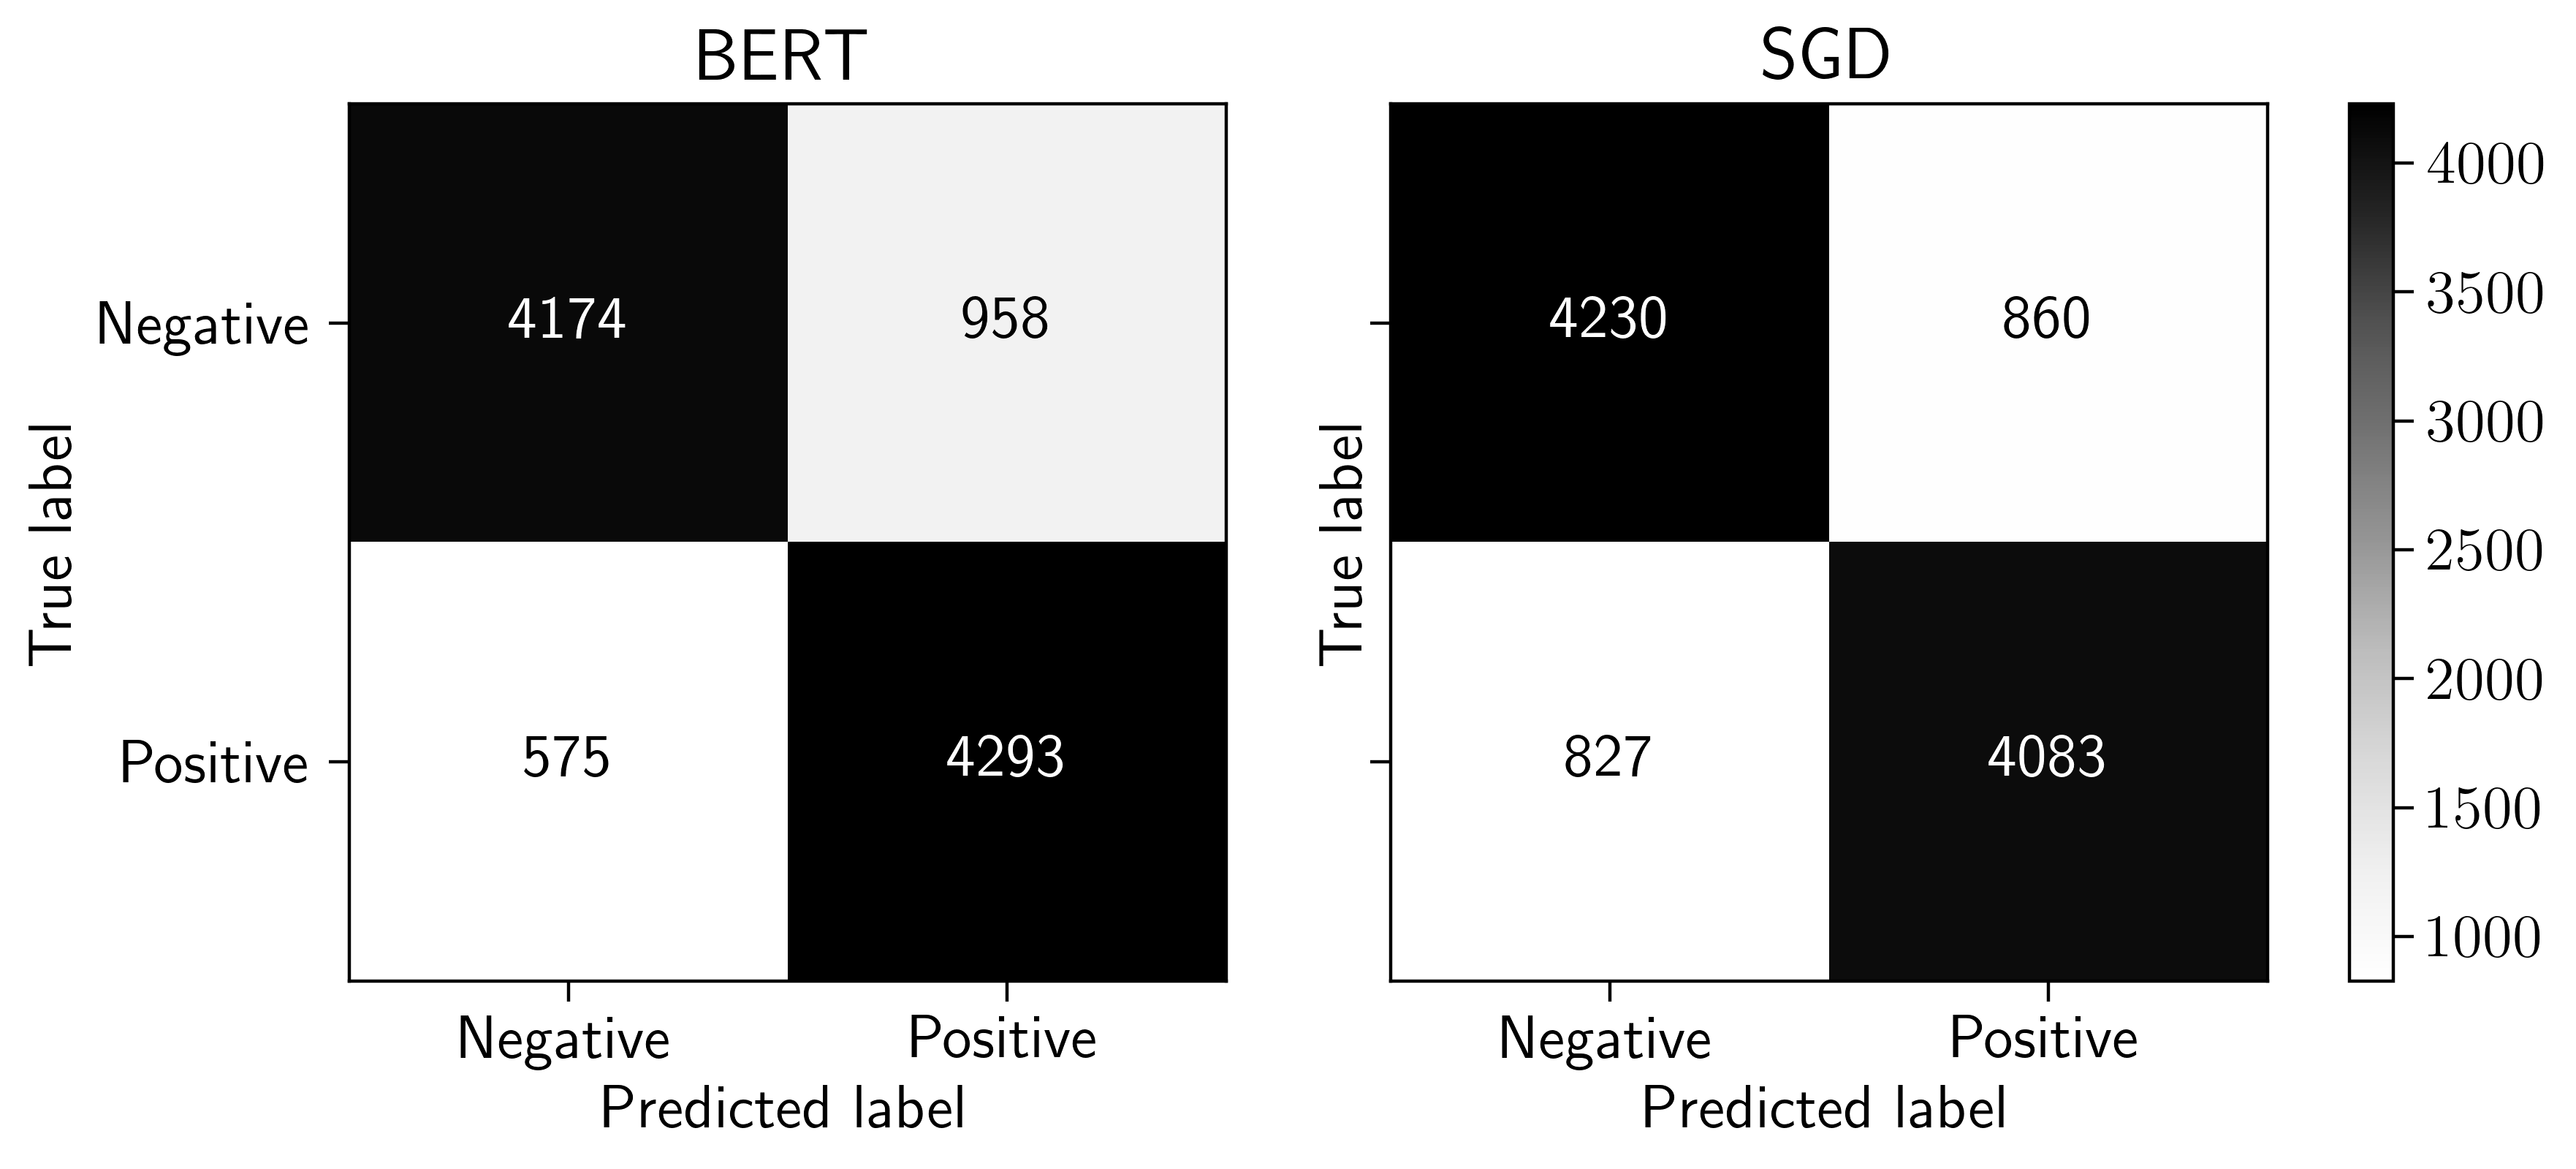
\includegraphics[width=0.85\textwidth]{figures/06_results/01_rfp/01_pol/01_cm/eng_eq_any.png}
    \caption{Confusion matrices for balanced, English, any length sample.}
    \label{fig:Res_RF_Pol_CM_EBA}
\end{figure}

Although not shown in this section, the confusion matrices for the balanced, multilingual, any length sample bear a close resemblance to those shown in Figure \ref{fig:Res_RF_Pol_CM_EBA}. The main difference between the two is in the total number of mistakes made as opposed to the manner in which those mistakes were made, eg labelling a positive review as negative.

The confusion matrices for the balanced, English, long sample are shown in Figure \ref{fig:Res_RF_Pol_CM_EBL}. The results for the SGD classifier are very similar to its results in Figure \ref{fig:Res_RF_Pol_CM_EBA}. However, the results for the BERT classifier are quite conspicuous: a significant number of mistakes are made by incorrectly classifying negative reviews as positive. It appears that, for long reviews, the BERT model's tendency to mislabel negatives as positives becomes even more pronounced.

\begin{figure}[ht]
    \centering
    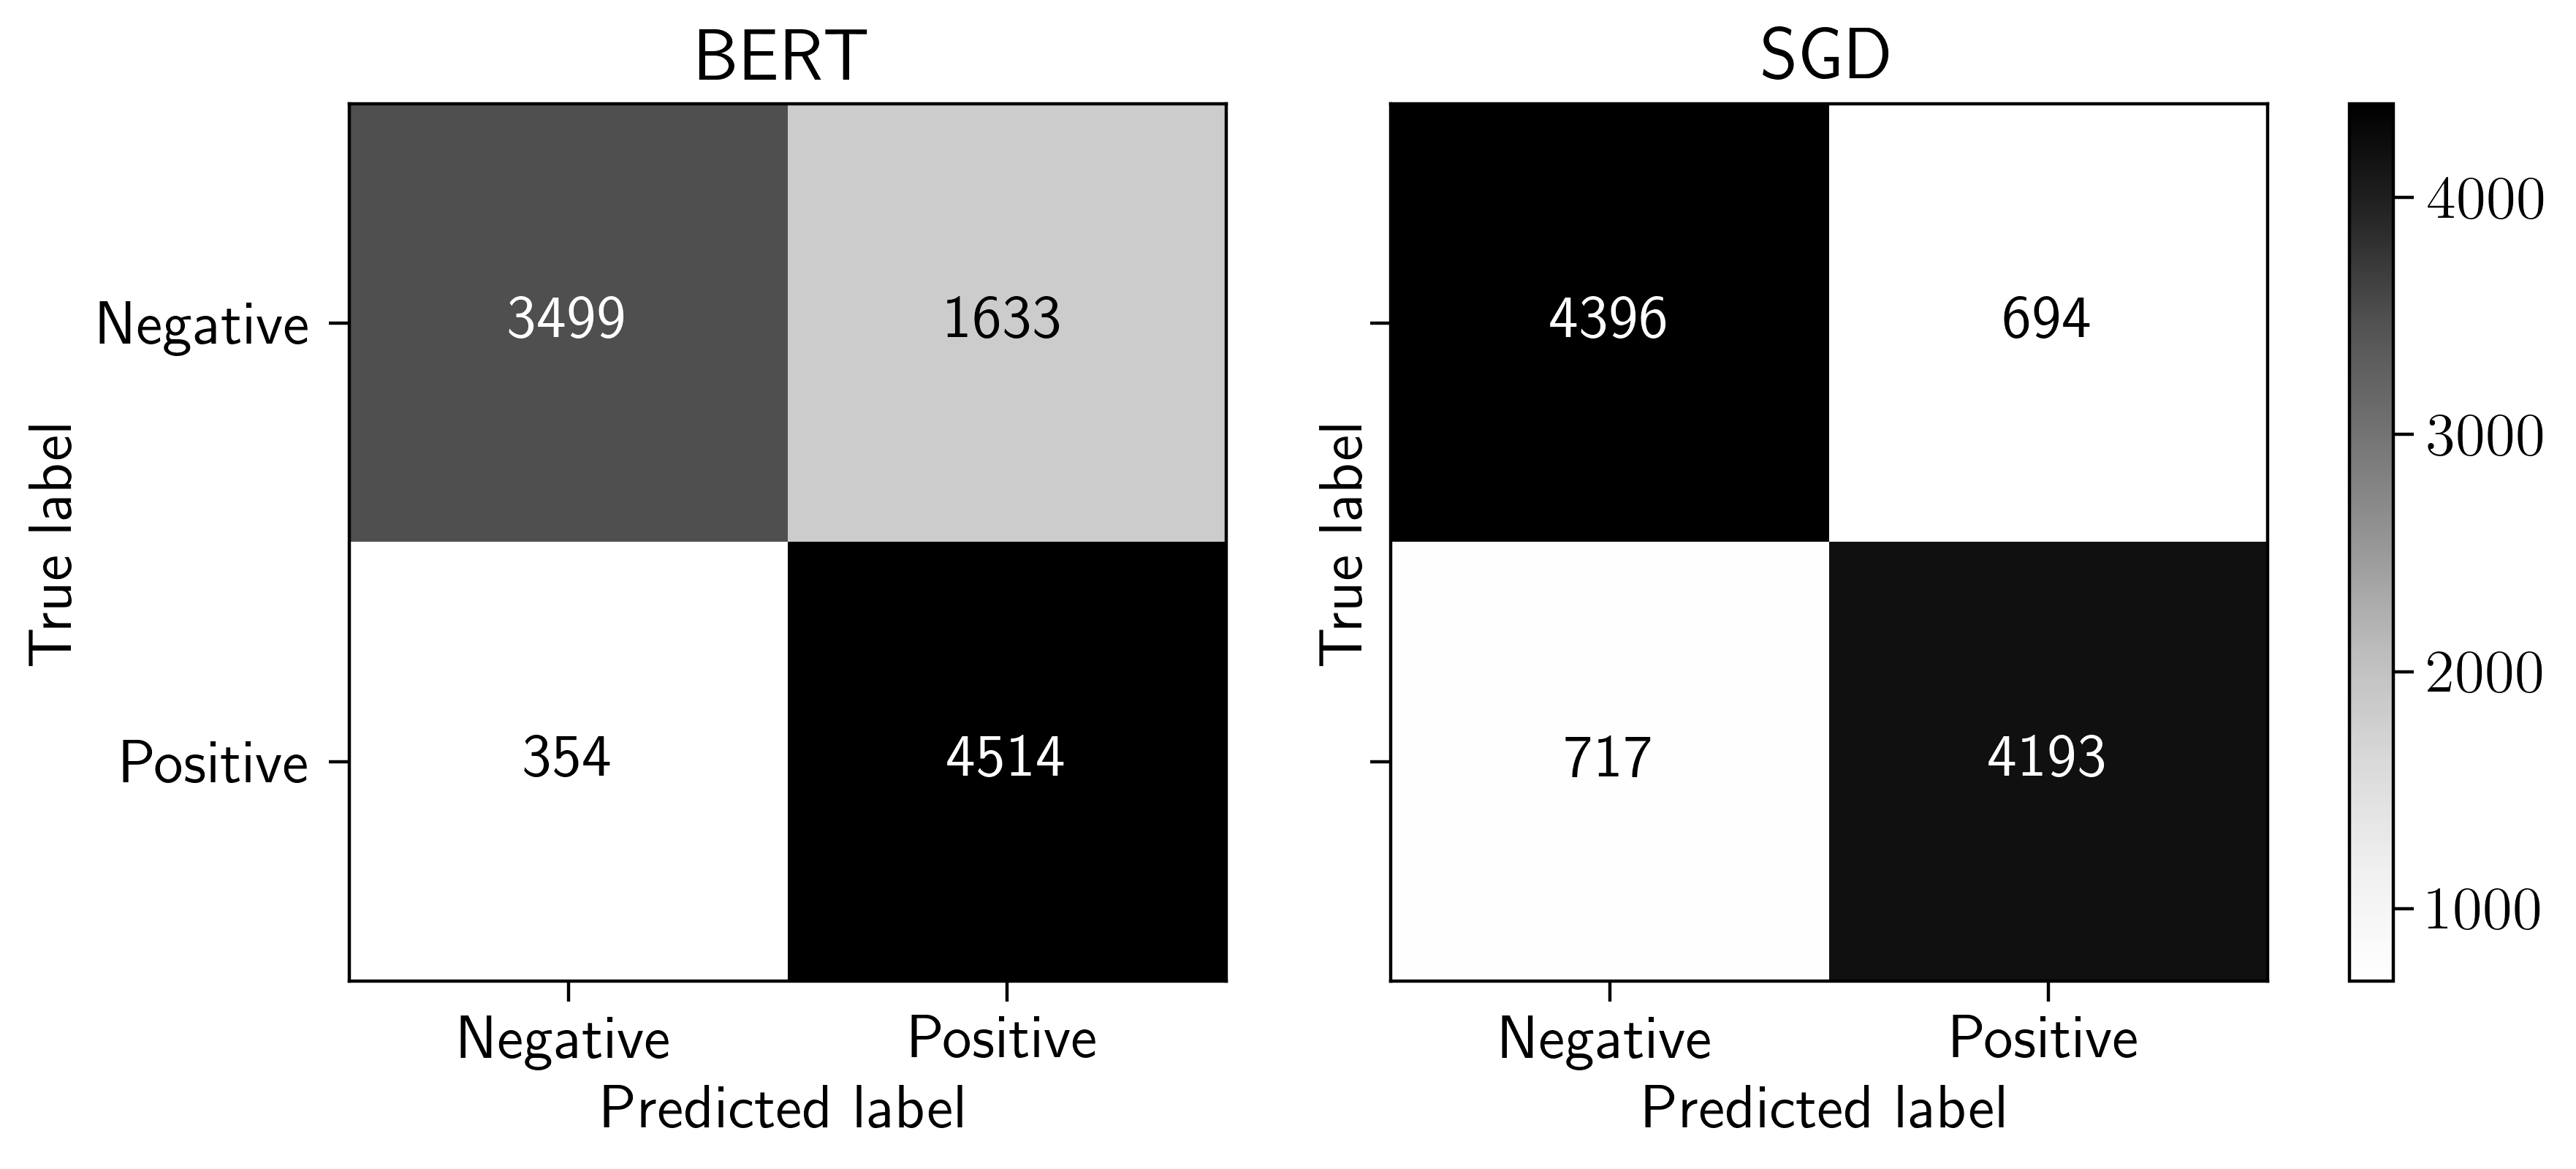
\includegraphics[width=0.85\textwidth]{figures/06_results/01_rfp/01_pol/01_cm/eng_eq_long.png}
    \caption{Confusion matrices for balanced, English, long sample.}
    \label{fig:Res_RF_Pol_CM_EBL}
\end{figure}

An additional example of BERT's performance against long reviews, for the imbalanced, English sample, can be seen in Figure \ref{fig:Res_RF_Pol_CM_EIL}. The LSVC classifier performs a good deal better than BERT due to the latter's previously highlighted tendency.

\begin{figure}[ht]
    \centering
    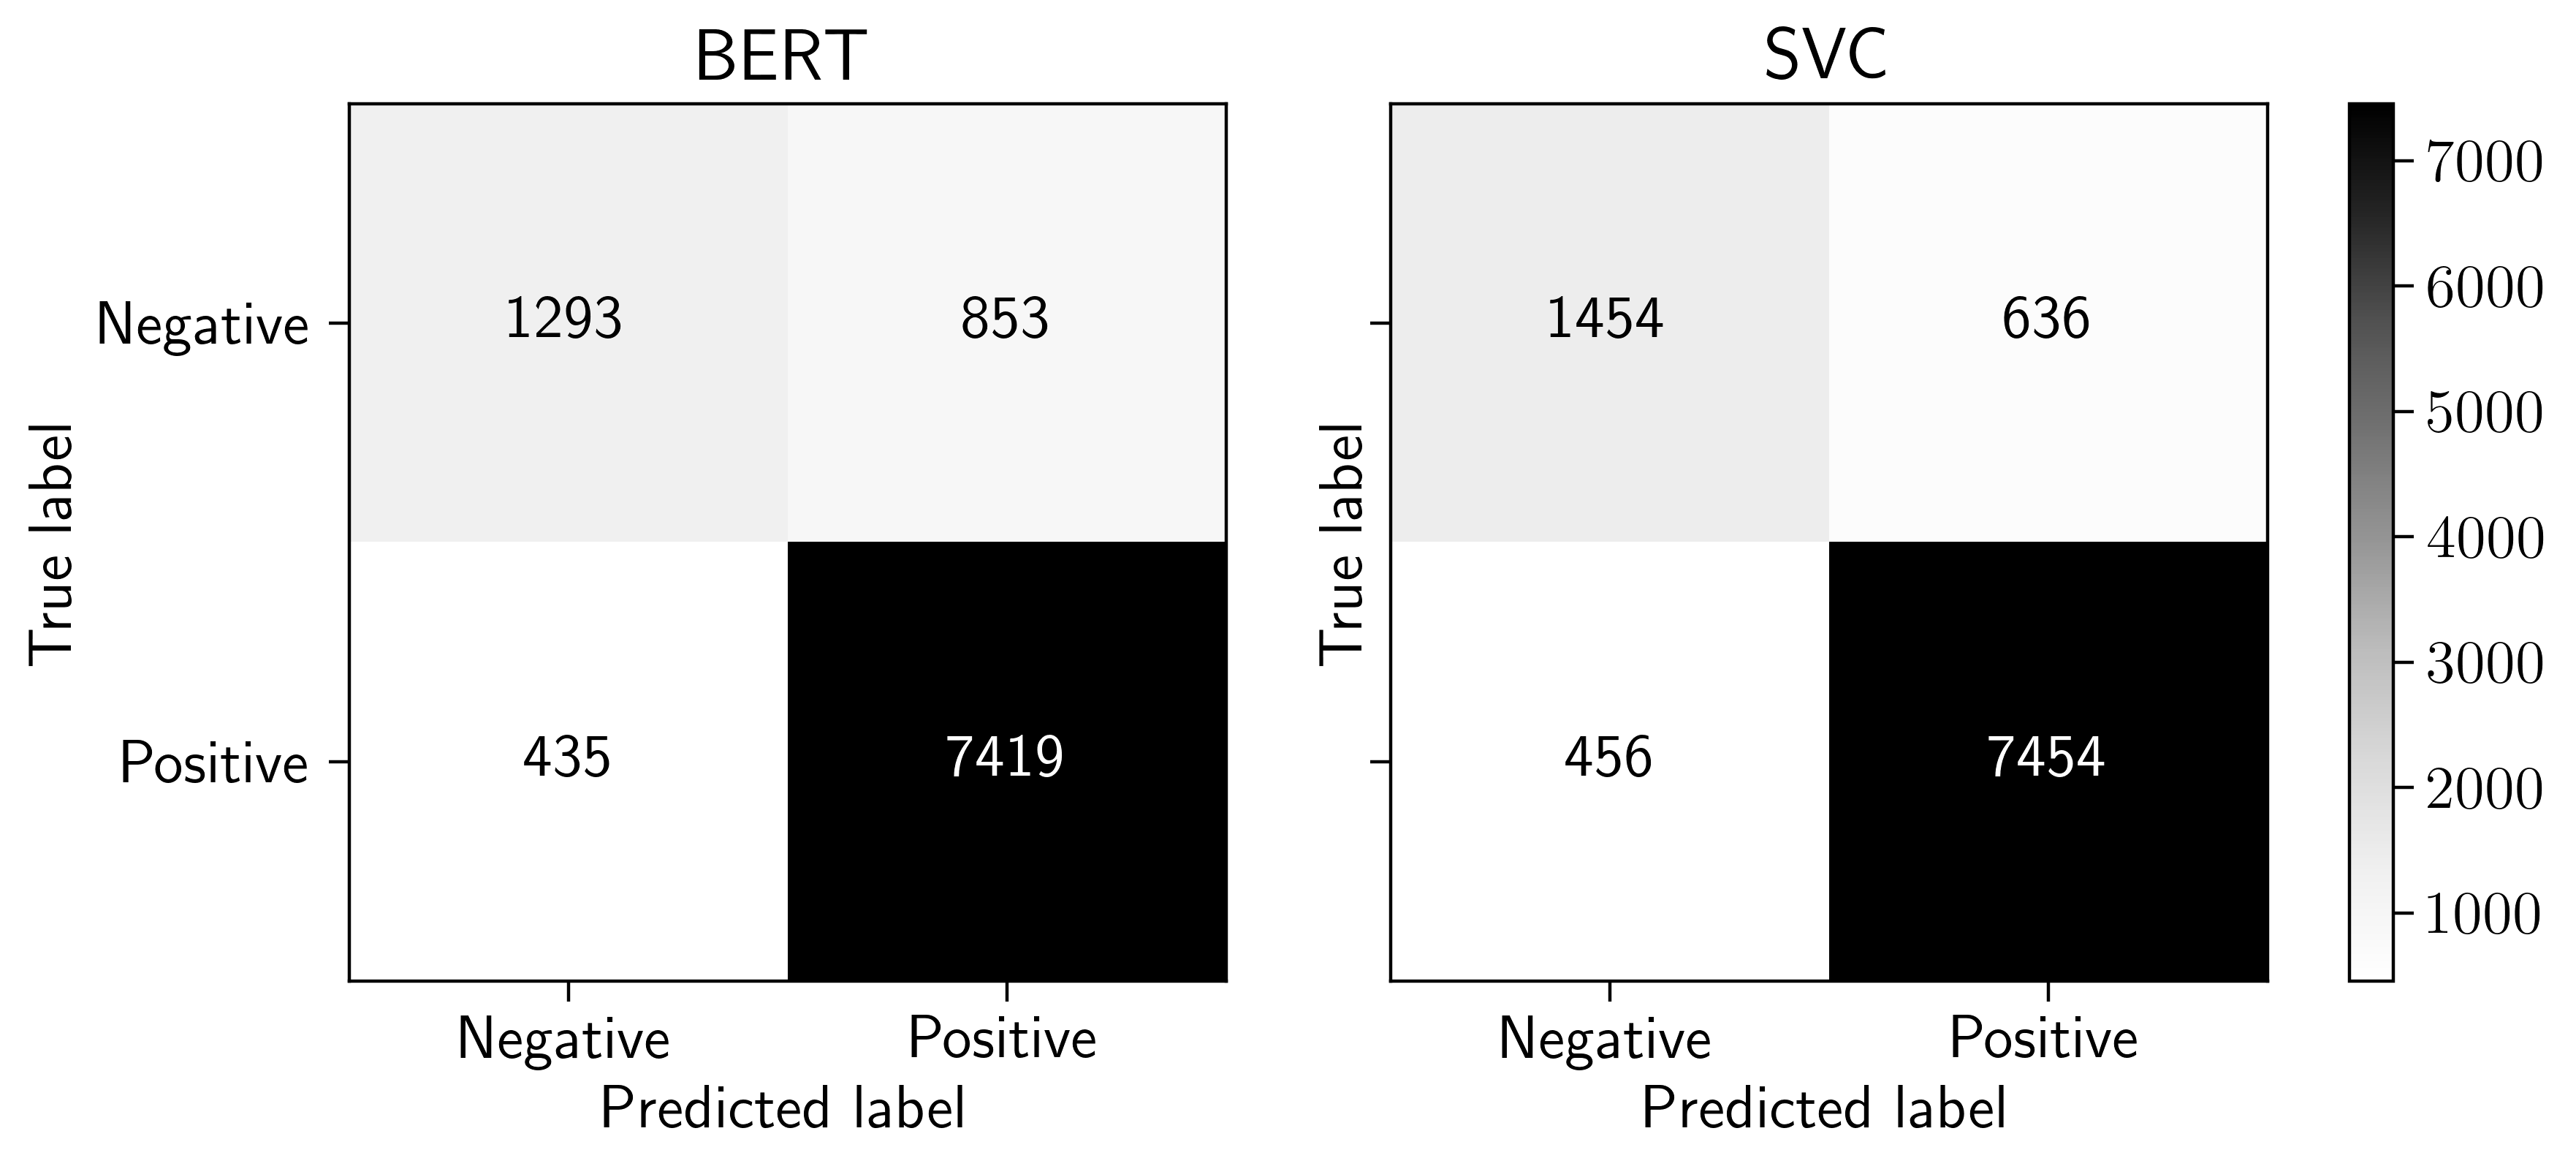
\includegraphics[width=0.85\textwidth]{figures/06_results/01_rfp/01_pol/01_cm/eng_any_long.png}
    \caption{Confusion matrices for imbalanced, English, long sample.}
    \label{fig:Res_RF_Pol_CM_EIL}
\end{figure}

\subsubsection{ROC Curves}

As was the case with the confusion matrices, selected ROC curves will be presented to help illustrate the performances of the trained models. A full collection of ROC curves can be found in Appendix \ref{sec:A1_ROC}.

The ROC curves and accompanying AUC values for both the balanced and imbalanced, English, any length samples can be seen in Figures \ref{fig:Res_RF_Pol_ROC_EBA} and \ref{fig:Res_RF_Pol_ROC_EIA}, respectively. By using the baseline as a comparison, these two plots provide a clear depiction of the predictive performances of both the BERT and optimal non-BERT models, regardless of the balanced or imbalanced nature of the dataset. In both examples, the BERT model outperforms the SGD model. This difference in performance can be seen in both the curves themselves, as well as in the corresponding AUC values.

\begin{figure}[ht]
    \centering
    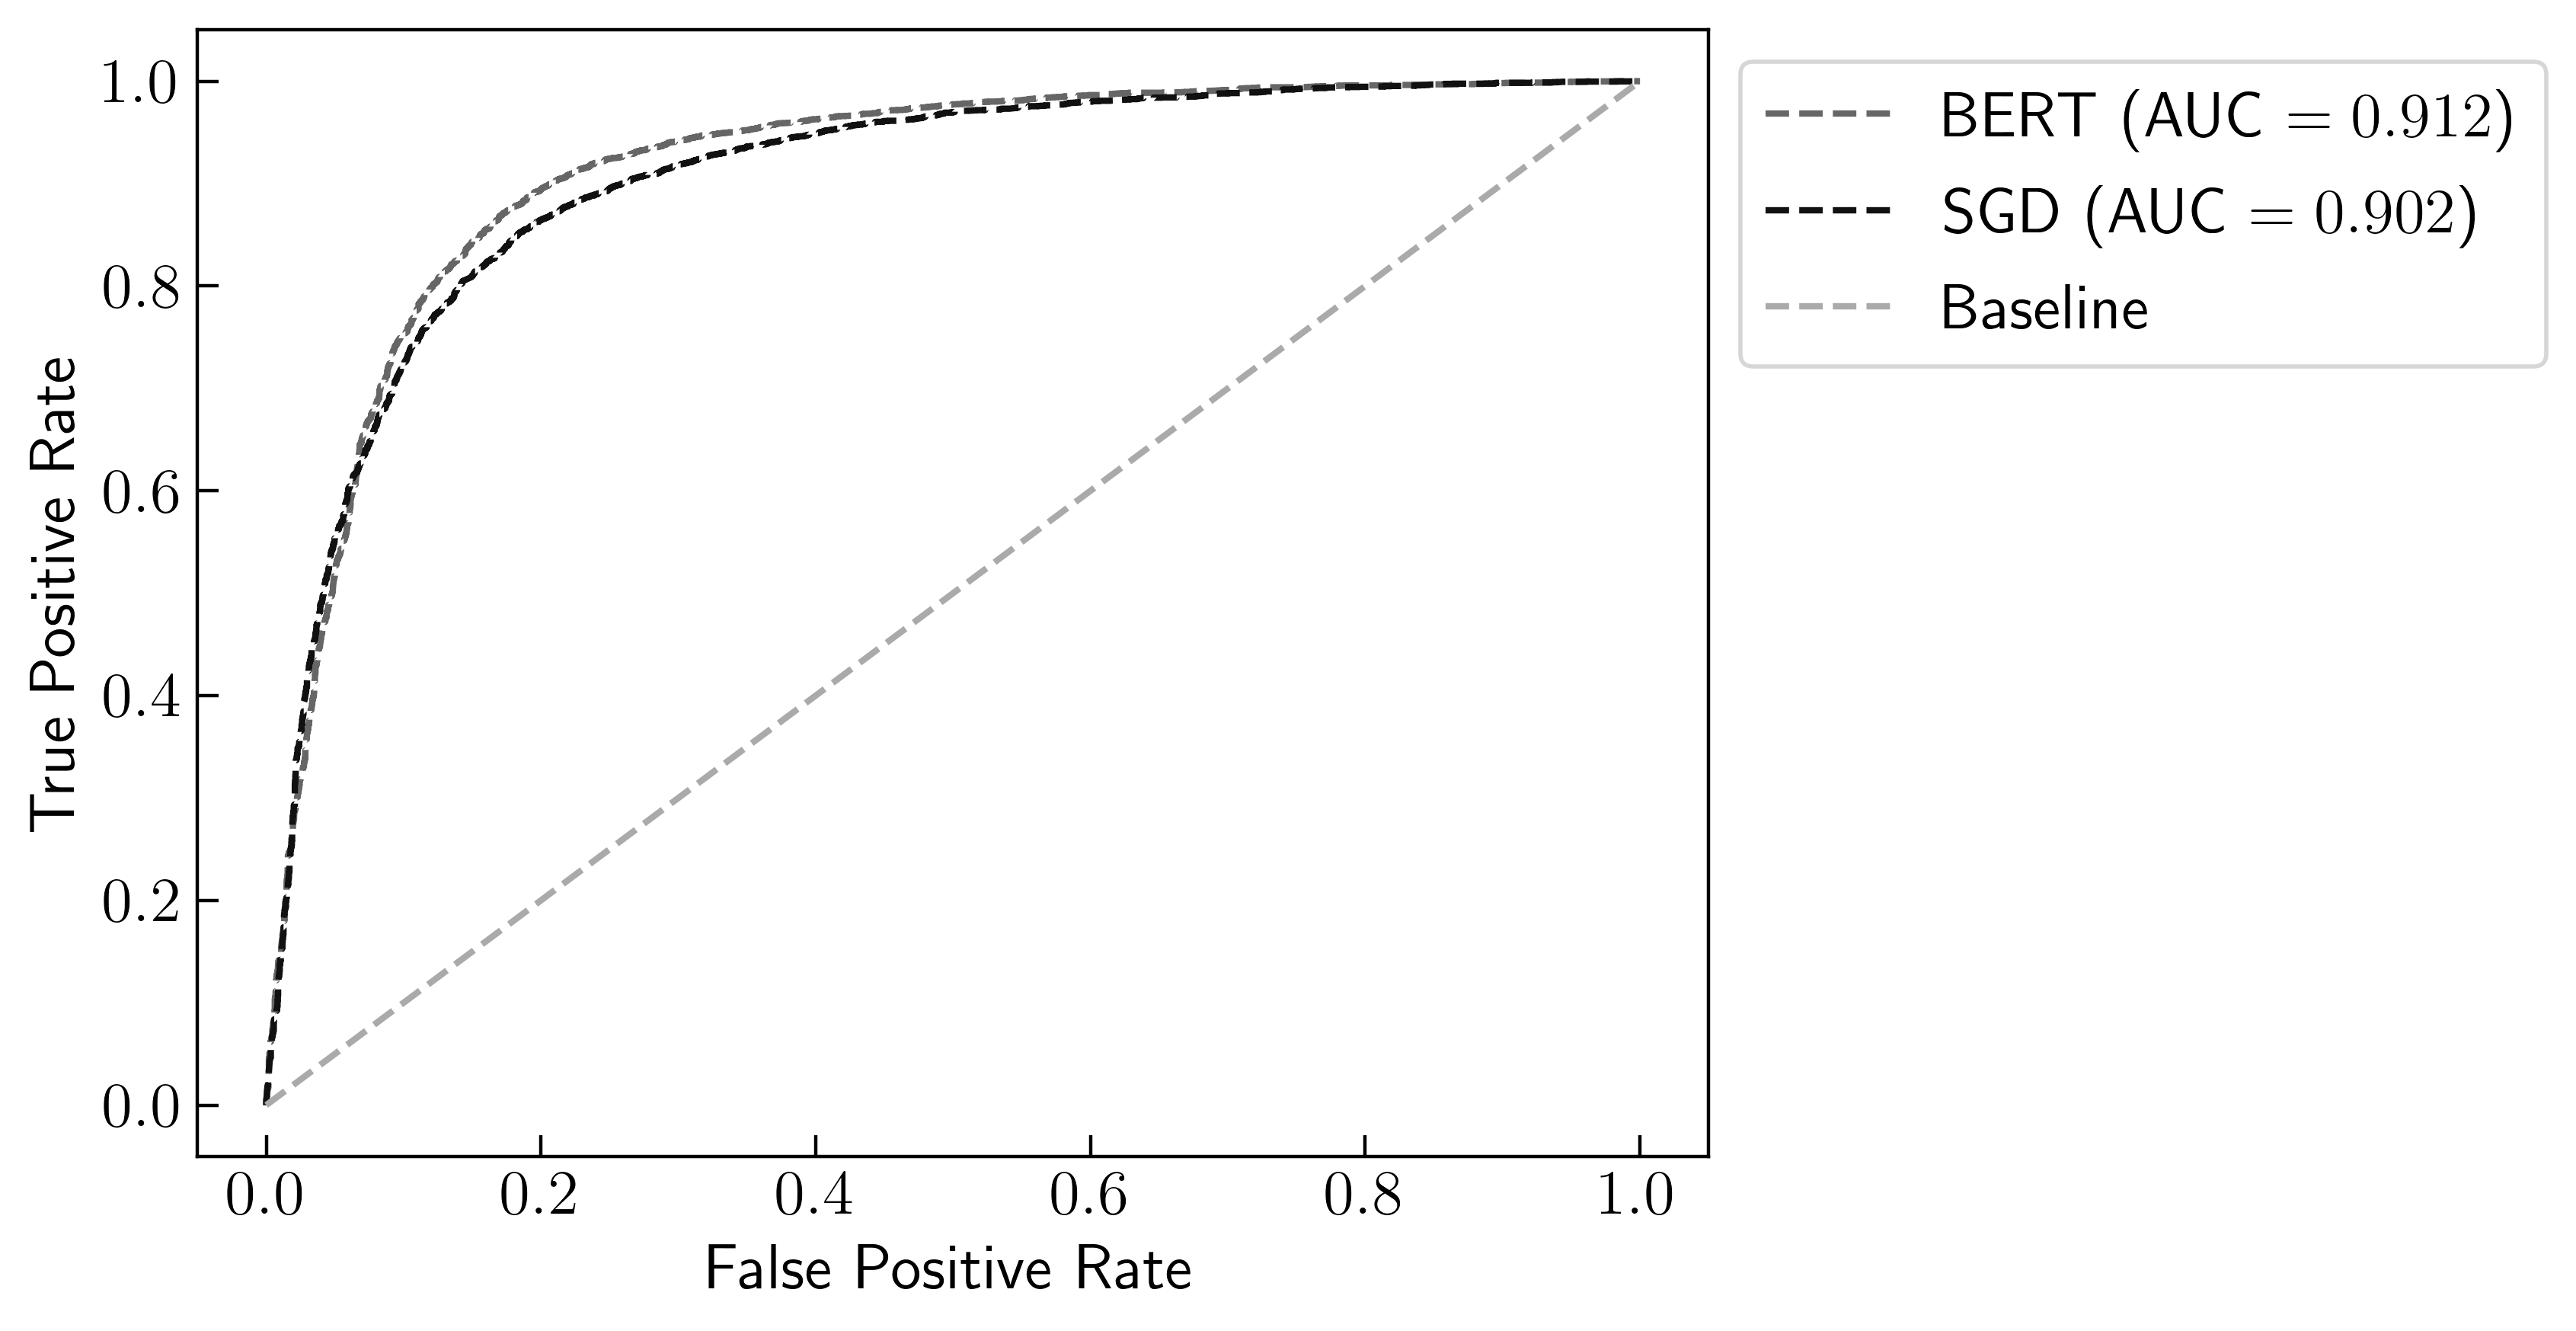
\includegraphics[width=0.85\textwidth]{figures/06_results/01_rfp/01_pol/02_roc/eng_eq_any.png}
    \caption{ROC curves and AUC values for balanced, English, any length sample.}
    \label{fig:Res_RF_Pol_ROC_EBA}
\end{figure}

\begin{figure}[ht]
    \centering
    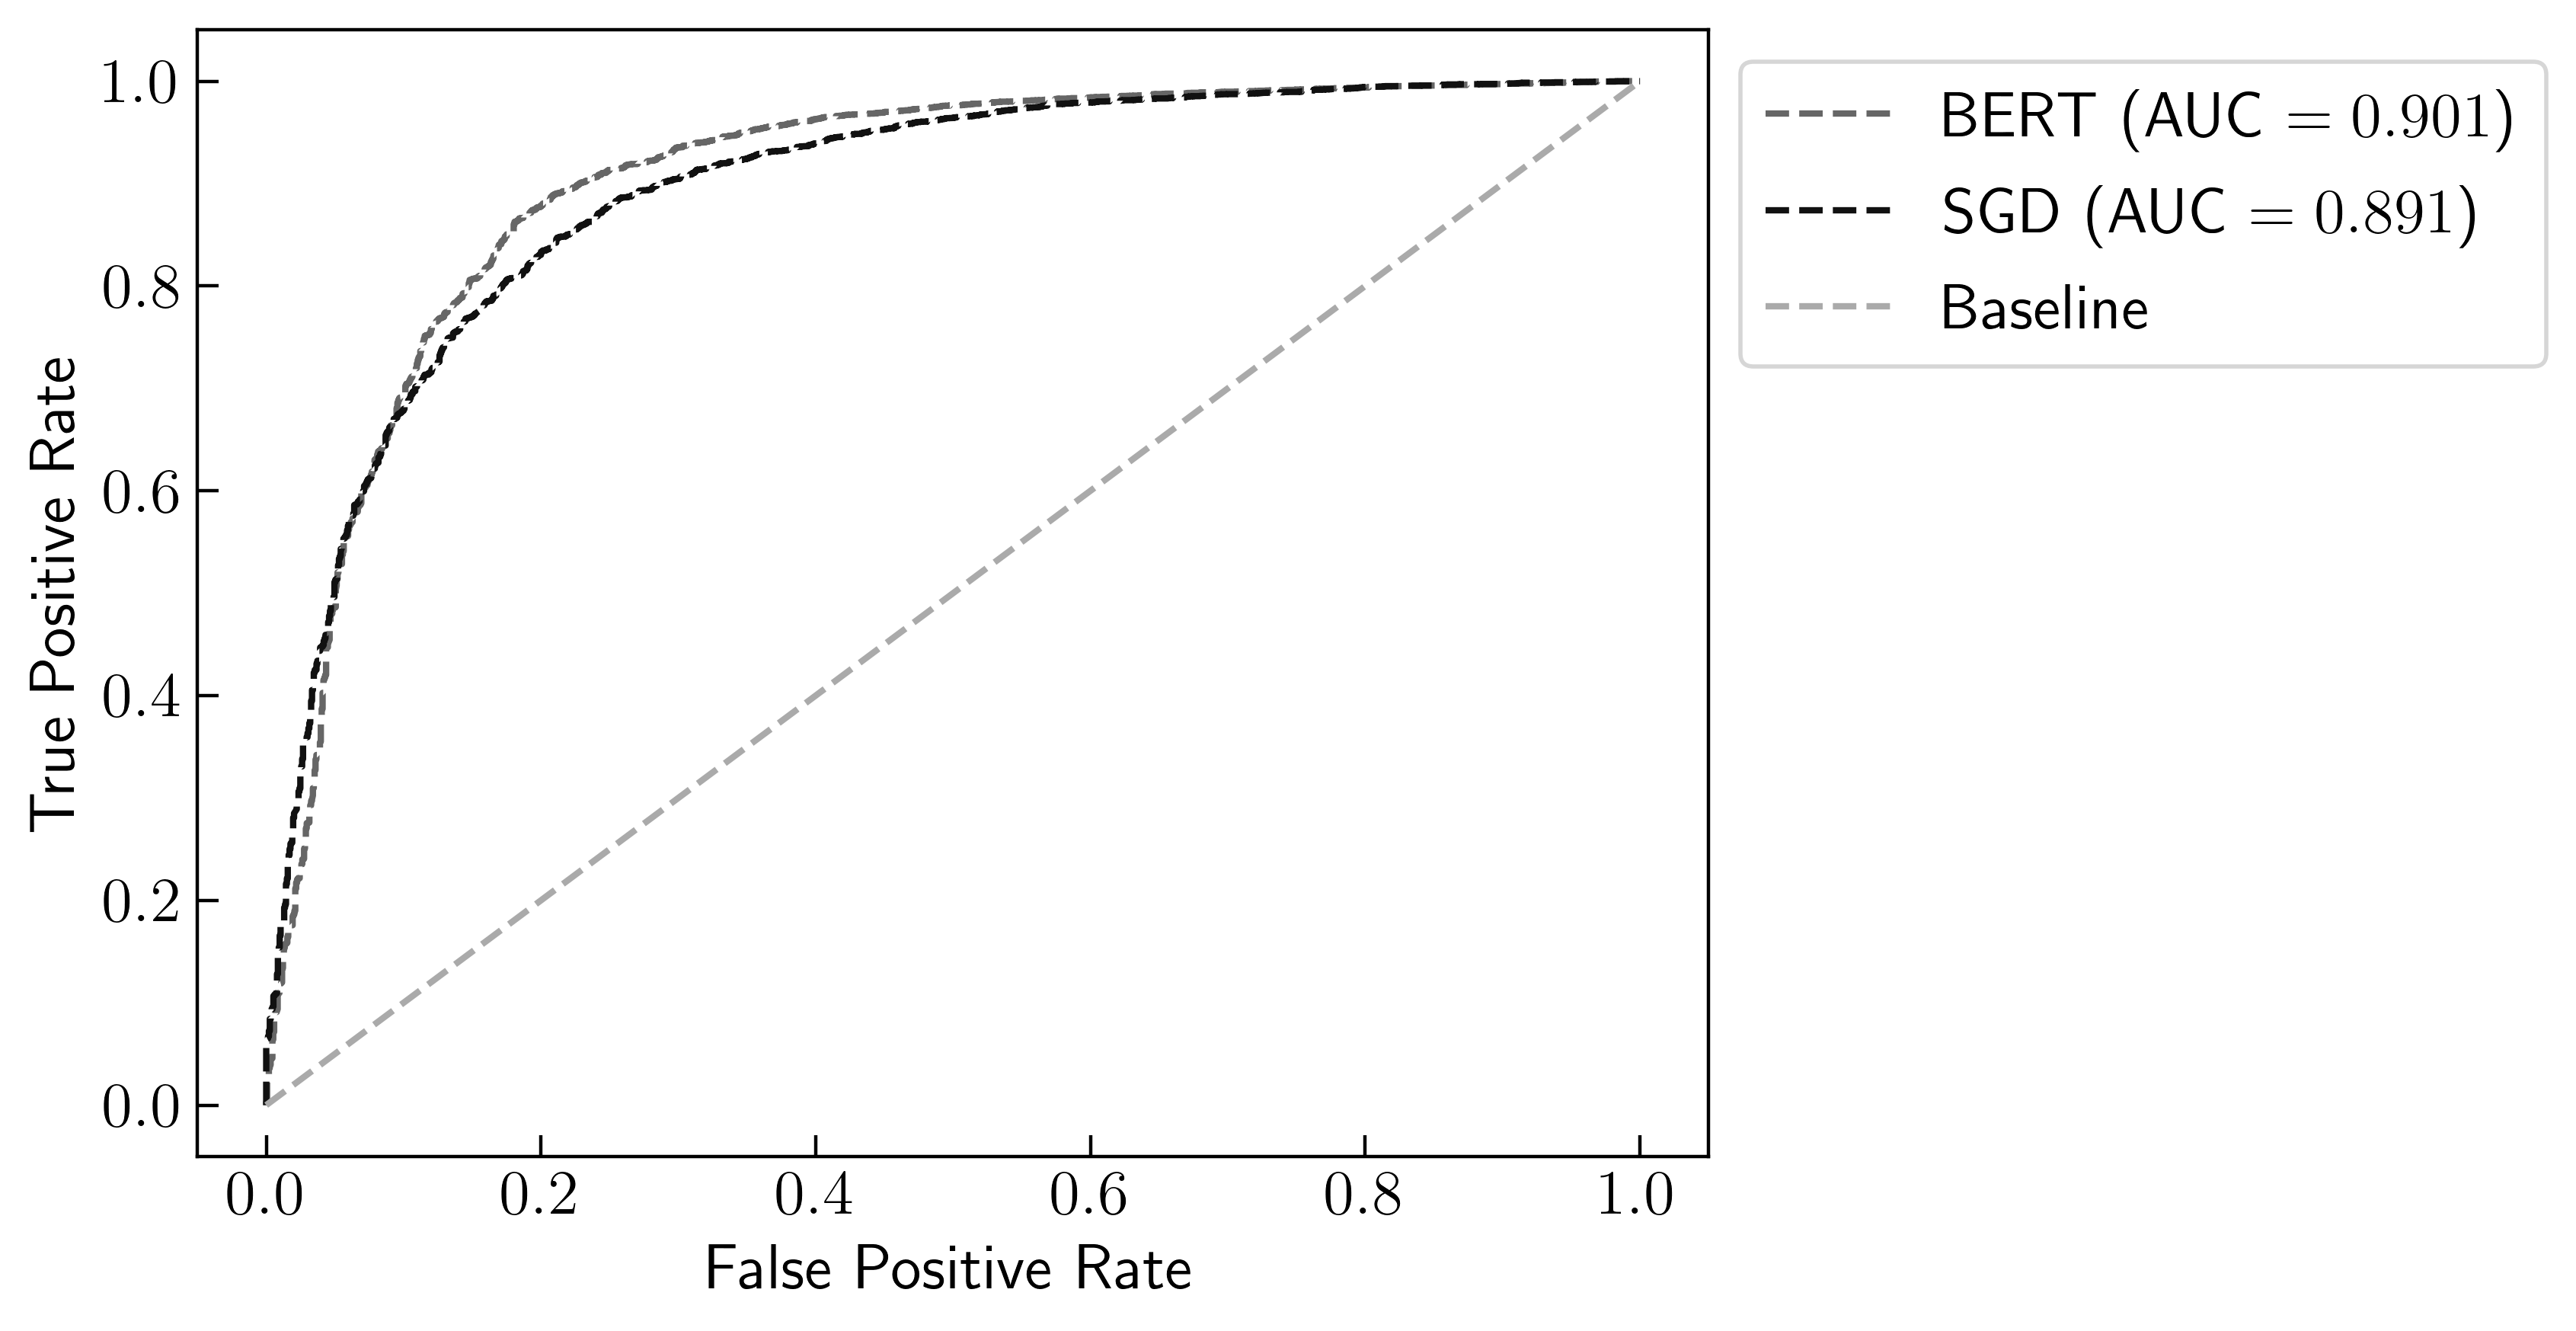
\includegraphics[width=0.85\textwidth]{figures/06_results/01_rfp/01_pol/02_roc/eng_any_any.png}
    \caption{ROC curves and AUC values for imbalanced, English, any length sample.}
    \label{fig:Res_RF_Pol_ROC_EIA}
\end{figure}

The other ROC curves, though not shown in this section, tend to show similar results, albeit with a few differences: the multilingual samples produce slightly poorer results, the non-BERT model generally outperforms BERT in long review samples and BERT generally outperforms the non-BERT model in short review samples.

\subsection{Votes} \label{sec:Res_RF_Votes}

In this section, the performances of the models trained to predict the number of votes that reviews received will be evaluated and discussed. Out of the two baseline regressors outlined in section \ref{sec:DI_RF_Votes}, the `mean' baseline (BM) was used as a comparison.

\subsubsection{Model Loss}

The MSE losses for each of the models, broken down by review language and length, can be seen in Table \ref{tab:Res_RF_Votes_CompLoss}.

\begin{table}[ht]
    \centering
    \begin{tabular}{l l | l l l l l}
        \toprule
        \textbf{Language} & \textbf{Length} & \textbf{BM} & \textbf{SGD} & \textbf{Ridge} & \textbf{LSVR} & \textbf{BERT}\\\midrule
        English&Any&$127.66$&$\mathbf{124.67}$&$124.74$&$124.81$&$155.7$\\
        English&Long&$67.12$&$64.74$&$64.76$&$65.24$&$\mathbf{50.03}$\\
        English&Short&$437.24$&$437.22$&$437.48$&$437.96$&$\mathbf{314.75}$\\\midrule
        Multilingual&Any&$480.85$&$466.56$&$\mathbf{466.31}$&$470.09$&$569.04$\\
        Multilingual&Long&$62.13$&$60.05$&$60.01$&$\mathbf{60.0}$&$68.54$\\
        Multilingual&Short&$335.32$&$334.02$&$334.25$&$336.69$&$\mathbf{264.81}$\\
        \bottomrule
    \end{tabular}
    \caption{Comparison of model test losses (MSE) for all samples.}
    \label{tab:Res_RF_Votes_CompLoss}
\end{table}

The resulting losses tend to be very large, with the optimal model not appearing to perform too much better than the baseline. The losses produced by the BERT models are quite extreme. For three of the samples, BERT produces results that are a good deal better than all of the other models; for the remaining samples, BERT produces the worst results by far, even when compared to the baseline.

Given these results, it does not appear that the trained models are very capable of predicting the number of votes that reviews received. The smallest losses were produced by the models trained on the long samples; however, considering that the accompanying baseline losses were equally small, these results do not seem too promising, either.

\subsubsection{Model Fit}

The $R^2$ scores for each of the models can be seen in Table \ref{tab:Res_RF_Votes_CompFit}.

\begin{table}[ht]
    \centering
    \begin{tabular}{l l | l l l l l}
        \toprule
        \textbf{Language} & \textbf{Length} & \textbf{BM} & \textbf{SGD} & \textbf{Ridge} & \textbf{LSVR} & \textbf{BERT}\\\midrule
        English&Any&$0.0$&$\mathbf{0.02}$&$0.02$&$0.02$&$0.01$\\
        English&Long&$0.0$&$\mathbf{0.04}$&$0.04$&$0.03$&$0.0$\\
        English&Short&$\mathbf{0.0}$&$0.0$&$0.0$&$0.0$&$-0.01$\\\midrule
        Multilingual&Any&$0.0$&$0.03$&$\mathbf{0.03}$&$0.02$&$0.0$\\
        Multilingual&Long&$0.0$&$0.03$&$0.03$&$\mathbf{0.03}$&$-0.02$\\
        Multilingual&Short&$0.0$&$0.0$&$0.0$&$0.0$&$\mathbf{0.01}$\\
        \bottomrule
    \end{tabular}
    \caption{Comparison of model test fits ($R^2$) for all samples.}
    \label{tab:Res_RF_Votes_CompFit}
\end{table}

Based on these results, it becomes abundantly clear that none of the trained models were predicting the number of votes that reviews received in an accurate manner. The model with the most accurate fit, the SGD regressor tested against the long, English sample, only produced an $R^2$ value of 0.04 - a result which is barely better than a baseline regressor. In fact, two of the BERT models even produced negative $R^2$ values.

\subsection{Playtime} \label{sec:Res_RF_PT}

In this section, the performances of the models trained to predict the amount of time that reviewers spent playing the games they reviewed will be evaluated and discussed.

\subsubsection{Model Loss}

The MSE losses for each of the models, broken down by review language and length, can be seen in Table \ref{tab:Res_RF_PT_CompLoss}.

\begin{table}[ht]
    \centering
    \begin{tabular}{l l | l l l l l}
        \toprule
        \textbf{Language} & \textbf{Length} & \textbf{BM} & \textbf{SGD} & \textbf{Ridge} & \textbf{LSVR} & \textbf{BERT}\\\midrule
        English&Any&$48.09$&$44.17$&$44.2$&$45.76$&$\mathbf{35.29}$\\
        English&Long&$71.96$&$\mathbf{60.69}$&$61.75$&$60.71$&$66.04$\\
        English&Short&$46.05$&$43.06$&$43.05$&$44.82$&$\mathbf{40.27}$\\\midrule
        Multilingual&Any&$44.36$&$\mathbf{41.29}$&$41.66$&$43.31$&$45.58$\\
        Multilingual&Long&$79.96$&$71.33$&$72.27$&$\mathbf{71.21}$&$98.75$\\
        Multilingual&Short&$34.79$&$33.09$&$33.22$&$34.93$&$\mathbf{28.06}$\\
        \bottomrule
    \end{tabular}
    \caption{Comparison of model test losses (MSE) for all samples.}
    \label{tab:Res_RF_PT_CompLoss}
\end{table}

The losses, though not as high as those of the vote prediction models, are still quite large. For each sample, the optimal trained model does not appear to perform too much better than the baseline does. As was the case with the review votes, the BERT models tend to produce extreme results. For three of the sample, BERT performs the strongest; for two of the samples, BERT performs a good deal worse than the baseline. Only one of the samples, the long, English one, sees BERT producing moderate results.

Given these results, it appears that the trained models are not capable of predicting the playtime of the reviewers to a significant degree. However, the results do not seem quite as bad as those of the vote prediction models.

\subsubsection{Model Fit}

The $R^2$ scores for each of the models can be seen in Table \ref{tab:Res_RF_PT_CompFit}.

\begin{table}[ht]
    \centering
    \begin{tabular}{l l | l l l l l}
        \toprule
        \textbf{Language} & \textbf{Length} & \textbf{BM} & \textbf{SGD} & \textbf{Ridge} & \textbf{LSVR} & \textbf{BERT}\\\midrule
        English&Any&$0.0$&$0.08$&$0.08$&$0.05$&$\mathbf{0.09}$\\
        English&Long&$0.0$&$\mathbf{0.16}$&$0.14$&$0.16$&$0.14$\\
        English&Short&$0.0$&$0.07$&$0.07$&$0.03$&$\mathbf{0.08}$\\\midrule
        Multilingual&Any&$0.0$&$\mathbf{0.07}$&$0.06$&$0.02$&$0.04$\\
        Multilingual&Long&$0.0$&$0.11$&$0.1$&$\mathbf{0.11}$&$0.02$\\
        Multilingual&Short&$0.0$&$\mathbf{0.05}$&$0.05$&$0.0$&$0.03$\\
        \bottomrule
    \end{tabular}
    \caption{Comparison of model test fits ($R^2$) for all samples.}
    \label{tab:Res_RF_PT_CompFit}
\end{table}

Based on these results, it appears that, at least for the long samples, the trained models are able to fit the review data to a very small degree. For example, the largest $R^2$ score, $0.16$, is most likely an indication that the trained model, though better than a baseline, is only fitting the dataset weakly. In summary, using only the review text and scaled playtime values, the optimal models were only able to find a very weak correlation between the two features.

\subsection{Discussion}

\subsubsection{Polarity}

The results gathered from the polarity prediction models were very promising. For the balanced dataset samples, the BERT and optimal alternative models performed extremely well. The best performing models resulted in accuracies as high as 85.9\%, compared to a baseline of 49.1\%. The optimal models also performed strongly when tested against the imbalanced samples, and, even though the results were not quite as impressive, they still significantly outperformed the baseline classifiers.

The models tested against the English-language samples were more accurate than those tested against the multilingual samples, regardless of the review length or the balancing of the data. These results are not at all surprising since the multilingual models need to determine the text characteristics that indicate a particular sentiment or polarity for numerous languages, each with different amounts of training data.

For the balanced samples, long reviews tended to produce the most accurate overall results - though not for BERT. Conversely, long reviews produced the least accurate results for the imbalanced samples, with the short review samples consistently performing best. The any length review samples tended to produce results that were somewhere in between the long and short samples.

BERT outperformed the optimal alternative models in two-thirds of the balanced sample tests. For the imbalanced samples, BERT produced the highest accuracy in the short and any length, English samples; however, it was beaten by both the SGD and LSVC models when tested against all three of the imbalanced, multilingual samples.

In cases where the BERT model performed the strongest, the difference in accuracy between it and the optimal alternative was rarely more than 1-2\%. However, in cases where the BERT model was beaten, the difference in accuracy between it and the alternative was a bit more extreme, ranging from 1\% to almost 7\%.

These results indicate that, regardless of the language or the distribution of the reviews, both the trained BERT and alternative models are highly capable of making accurate predictions concerning the review polarity based solely on the review text. Although the BERT models did not reliably outperform the optimal alternatives, it is worth noting that only a relatively small number of data points were used to train, validate and test each of the individual BERT models. Given that BERT tends to perform better when trained with large amounts of data, and given the abundance of untested reviews contained within the dataset, it seems certain that more accurate models could be developed by expanding upon the work discussed in this report.

\subsubsection{Votes}

The results gathered from the models trained to predict the number of votes clearly indicated that neither BERT nor the alternative models were capable of predicting individual outcomes any better than a baseline regressor was. This result remained consistent across all of the dataset samples.

Nonetheless, further investigation into this approach may be worthwhile. As was discussed in section \ref{sec:LR_NLP_Help}, reviews could be classified based on the number of votes they received, eg top 10\% of reviews, top 20\% of reviews, etc. Another approach might be to exclude reviews that did not receive any votes, a majority of the dataset, in order to balance the sampled data. Finally, additional data balancing could be implemented by selecting an equal number of reviews with, for example, 0-5 votes, 5-20 votes, 20-100 votes, etc.

\subsubsection{Playtime}

The results gathered from the models trained to predict the playtime of reviewers were somewhat more promising than those gathered from the vote prediction models. However, at best, certain trained models were only able to determine a weak correlation between the review text and the resulting playtime.

As was the case with the vote prediction, further investigation may be worthwhile. A similar form of percentile-based classification could be tried, as could additional data balancing techniques.

\section{Representative Users} \label{sec:Res_RU}

In this section, the performances of the models trained to determine representative users will be evaluated and discussed.

\subsection{Overall Results}

The overall model performances, ie when evaluated using the entire test set and not on a per-user basis, will be compared in this section.

\subsubsection{Comparison of Models}

The predictive accuracies of each of the trained models will be detailed in this section. The `most frequent' baseline (BF) was used as a comparison. It is worth noting that, based on the methodology discussed in section \ref{sec:DI_RU}, accuracies that are significantly higher than the baseline result are not expected.

\paragraph{Six Rating Classes}

The English and multilingual model accuracies for the 6-class samples can be seen in Table \ref{tab:Res_PU_Comp6}.

\begin{table}[ht]
    \centering
    \begin{tabular}{l | l l l l l l}
        \toprule
        \textbf{Language} & \textbf{BF} & \textbf{MNB} & \textbf{CNB} & \textbf{SGD} & \textbf{LSVC} & \textbf{BERT}\\\midrule
        English&$0.468$&$0.494$&$0.484$&$0.538$&$0.534$&$\mathbf{0.543}$\\
        Multilingual&$0.515$&$0.523$&$0.485$&$\mathbf{0.539}$&$0.529$&$0.517$\\
        \bottomrule
    \end{tabular}
    \caption{Comparison of model test accuracy for 6-label classifiers.}
    \label{tab:Res_PU_Comp6}
\end{table}

Based on the BF accuracies, the distribution of classes appears to be quite imbalanced given that almost half of the English reviews are for a single class while an outright majority of multilingual reviews are for a single class.

Nonetheless, for the English sample, the BERT model resulted in an accuracy that was almost 8\% better than the baseline. The SGD and LSVC models also produced adequate results. The results for the multilingual sample were a good deal worse, however. The BERT model barely outperformed the baseline while the optimal model, the SGD classifier, only beat the baseline by 2.4\%.

\paragraph{Three Rating Classes}

The English and multilingual model accuracies for the 3-class samples can be seen in Table \ref{tab:Res_PU_Comp3}.

\begin{table}[ht]
    \centering
    \begin{tabular}{l | l l l l l l}
        \toprule
        \textbf{Language} & \textbf{BF} & \textbf{MNB} & \textbf{CNB} & \textbf{SGD} & \textbf{LSVC} & \textbf{BERT}\\\midrule
        English&$0.894$&$0.894$&$0.893$&$0.895$&$0.894$&$\mathbf{0.899}$\\
        Multilingual&$\mathbf{0.916}$&$0.916$&$0.852$&$0.916$&$0.915$&$0.904$\\
        \bottomrule
    \end{tabular}
    \caption{Comparison of model test accuracy for 3-label classifiers.}
    \label{tab:Res_PU_Comp3}
\end{table}

The distribution of classes in both of the 3-class samples is extremely imbalanced, with roughly 90\% of the reviews being assigned to a single class.

Given this severe imbalance, the poor performances of the trained models, relative to their baselines, are not at all surprising. For the English sample, the BERT model produced the best results, beating the baseline by a meagre 0.5\%. For the multilingual sample, none of the trained models were able to outperform the baseline.

\subsubsection{Classification Metrics}

In this section, classification results taken from the baseline, BERT and SGD classifiers will be presented. As was the case with review polarity prediction, the macro average and weighted average versions of each model's precision, recall and $F_1$-scores will be provided. The accuracies of the models will also be included for the sake of clarity.

\paragraph{Six Rating Classes}

The classification results for the 6-class samples and models can be seen in Table \ref{tab:Res_PU_Metric6}.

\begin{table}[ht]
    \centering
    \begin{tabular}{l l | c | c c c | c c c}
        \toprule
        \multirow{2}{*}{\textbf{Language}}&\multirow{2}{*}{\textbf{Model}}&\multirow{2}{*}{\textbf{Acc.}}&\multicolumn{3}{c}{\textbf{Macro Avg.}}&\multicolumn{3}{|c}{\textbf{Weighted Avg.}}\\
        &&&\textbf{Prec.} & \textbf{Rec.} & \textbf{$F_1$} & \textbf{Prec.} & \textbf{Rec.} & \textbf{$F_1$}\\\midrule
        English&BF&$0.47$&$0.08$&$0.17$&$0.11$&$0.22$&$0.47$&$0.30$\\
        English&SGD&$0.54$&$0.40$&$0.27$&$0.29$&$0.52$&$0.54$&$0.50$\\
        English&BERT&$\mathbf{0.54}$&$0.39$&$0.29$&$\mathbf{0.31}$&$0.53$&$0.54$&$\mathbf{0.52}$\\\midrule
        Multilingual&BF&$0.51$&$0.09$&$0.17$&$0.11$&$0.26$&$0.51$&$0.35$\\
        Multilingual&SGD&$\mathbf{0.54}$&$0.33$&$0.21$&$0.21$&$0.51$&$0.54$&$\mathbf{0.47}$\\
        Multilingual&BERT&$0.52$&$0.27$&$0.22$&$\mathbf{0.22}$&$0.47$&$0.52$&$0.47$\\
        \bottomrule
    \end{tabular}
    \caption{Model classification metrics for 6-class samples.}
    \label{tab:Res_PU_Metric6}
\end{table}

For the English sample, both sets of $F_1$-scores for the BERT and SGD models help to further indicate their sufficient, though not particularly impressive, performance. Both the macro and weighted average scores of the trained models are significantly higher than their baseline counterparts. As is expected given the imbalanced nature of the data, the weighted average results are a good deal higher than the macro average results.

The results for the multilingual sample are not quite as promising. Both sets of $F_1$-scores for the trained models do indicate a stronger performance, relative to their baselines, than the accuracy alone had suggested; although, this apparent increase appears to be due to the predictably poor precision score of the BF classifier hindering its $F_1$-scores.

\paragraph{Three Rating Classes}

The classification results for the 3-class samples and models can be seen in Table \ref{tab:Res_PU_Metric3}.

\begin{table}[ht]
    \centering
    \begin{tabular}{l l | c | c c c | c c c}
        \toprule
        \multirow{2}{*}{\textbf{Language}}&\multirow{2}{*}{\textbf{Model}}&\multirow{2}{*}{\textbf{Acc.}}&\multicolumn{3}{c}{\textbf{Macro Avg.}}&\multicolumn{3}{|c}{\textbf{Weighted Avg.}}\\
        &&&\textbf{Prec.} & \textbf{Rec.} & \textbf{$F_1$} & \textbf{Prec.} & \textbf{Rec.} & \textbf{$F_1$}\\\midrule
        English&BF&$0.89$&$0.30$&$0.33$&$0.31$&$0.80$&$0.89$&$0.84$\\
        English&SGD&$0.90$&$0.86$&$0.34$&$0.33$&$0.88$&$0.90$&$0.85$\\
        English&BERT&$\mathbf{0.90}$&$0.60$&$0.38$&$\mathbf{0.40}$&$0.87$&$0.90$&$\mathbf{0.87}$\\\midrule
        Multilingual&BF&$0.92$&$0.31$&$0.33$&$0.32$&$0.84$&$0.92$&$0.88$\\
        Multilingual&SGD&$\mathbf{0.92}$&$0.45$&$0.34$&$0.32$&$0.87$&$0.92$&$\mathbf{0.88}$\\
        Multilingual&BERT&$0.90$&$0.40$&$0.36$&$\mathbf{0.37}$&$0.87$&$0.90$&$0.88$\\
        \bottomrule
    \end{tabular}
    \caption{Model classification metrics for 3-class samples.}
    \label{tab:Res_PU_Metric3}
\end{table}

The classification metrics for the 3-class samples are not particularly informative or compelling. The values given for the trained models are practically identical to those given for the BF classifiers. The only significant differences occur in the macro averaged precision values; however, these differences are expected due to the imprecise nature of `most frequent' baseline classifiers.

\subsubsection{Confusion Matrices}

\paragraph{Six Rating Classes}

Confusion matrices for the 6-class, English sample can be seen in Figure \ref{fig:Res_PU_CM_E6}.

\begin{figure}[ht]
    \centering
    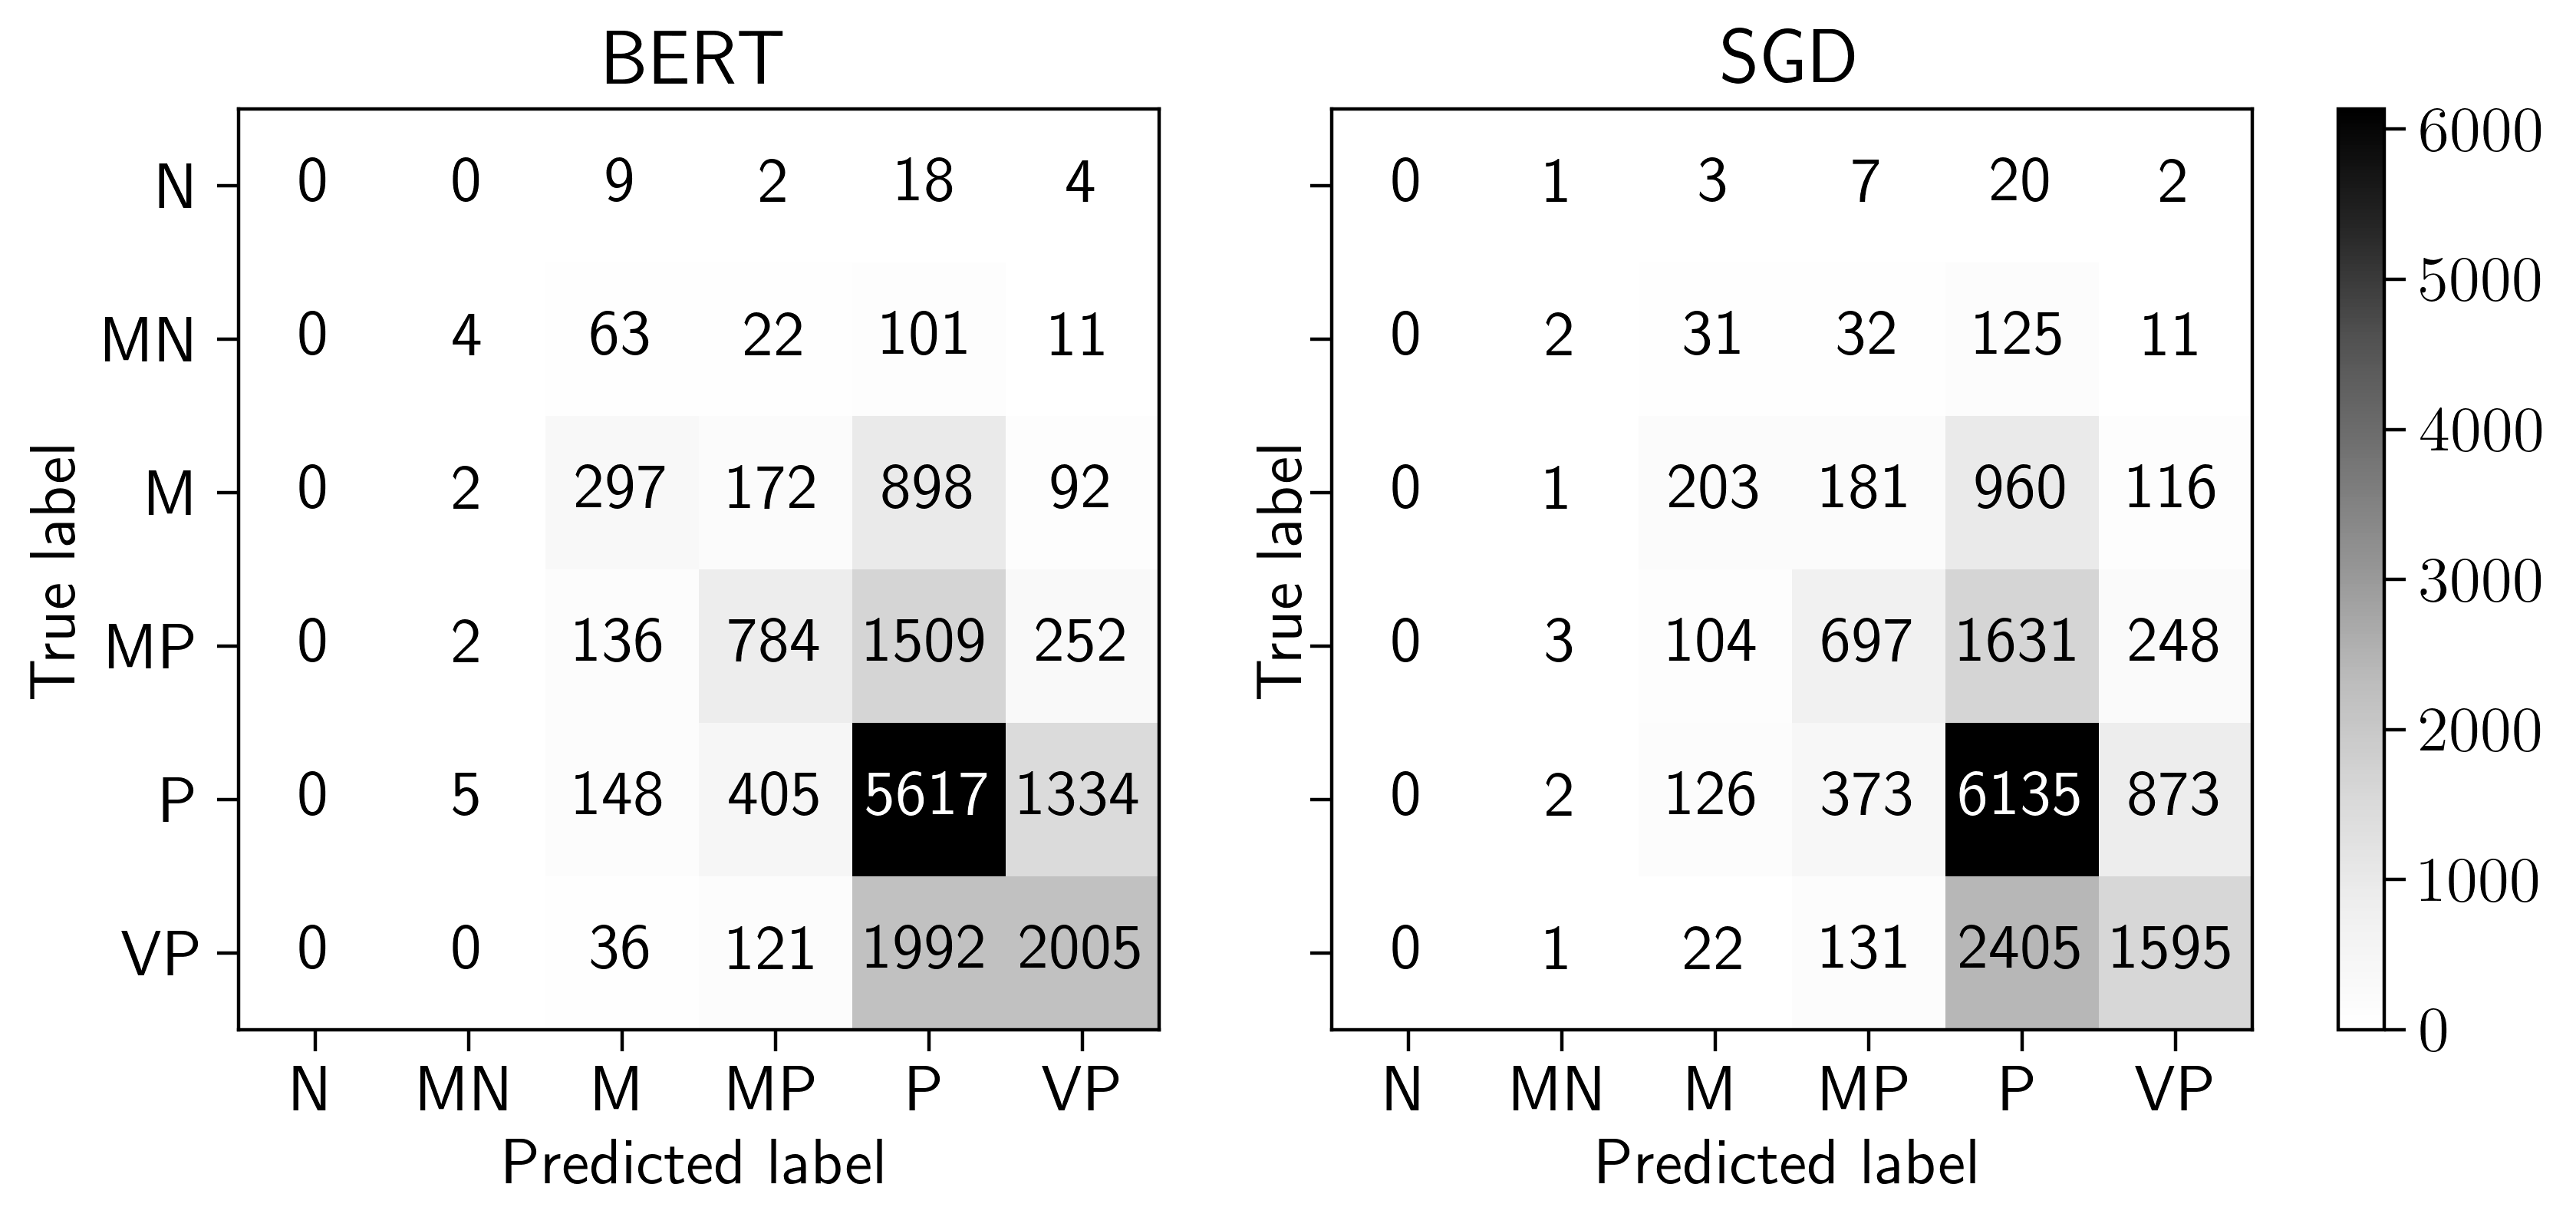
\includegraphics[width=0.85\textwidth]{figures/06_results/02_pu/01_cm/eng_6.png}
    \caption{Confusion matrices for 6-class, English sample.}
    \label{fig:Res_PU_CM_E6}
\end{figure}

As is to be expected, both classifiers predict the `positive' label most of the time, with the `very positive' label being predicted frequently as well. The BERT model appears to make accurate `very positive' classifications more often than the SGD model; although, it also misclassifies `positive' reviews as `very positive' more frequently, too.

The `negative' and `mostly negative' labels are almost never predicted by either model. The `mixed' reviews tend to be labelled as `positive' although accurate predictions are occasionally made, mainly by the BERT model. A similar effect appears to occur for the `mostly positive' label, with both models generally classifying such reviews as `positive'.

Confusion matrices for the 6-class, multilingual sample can be seen in Figure \ref{fig:Res_PU_CM_M6}.

\begin{figure}[ht]
    \centering
    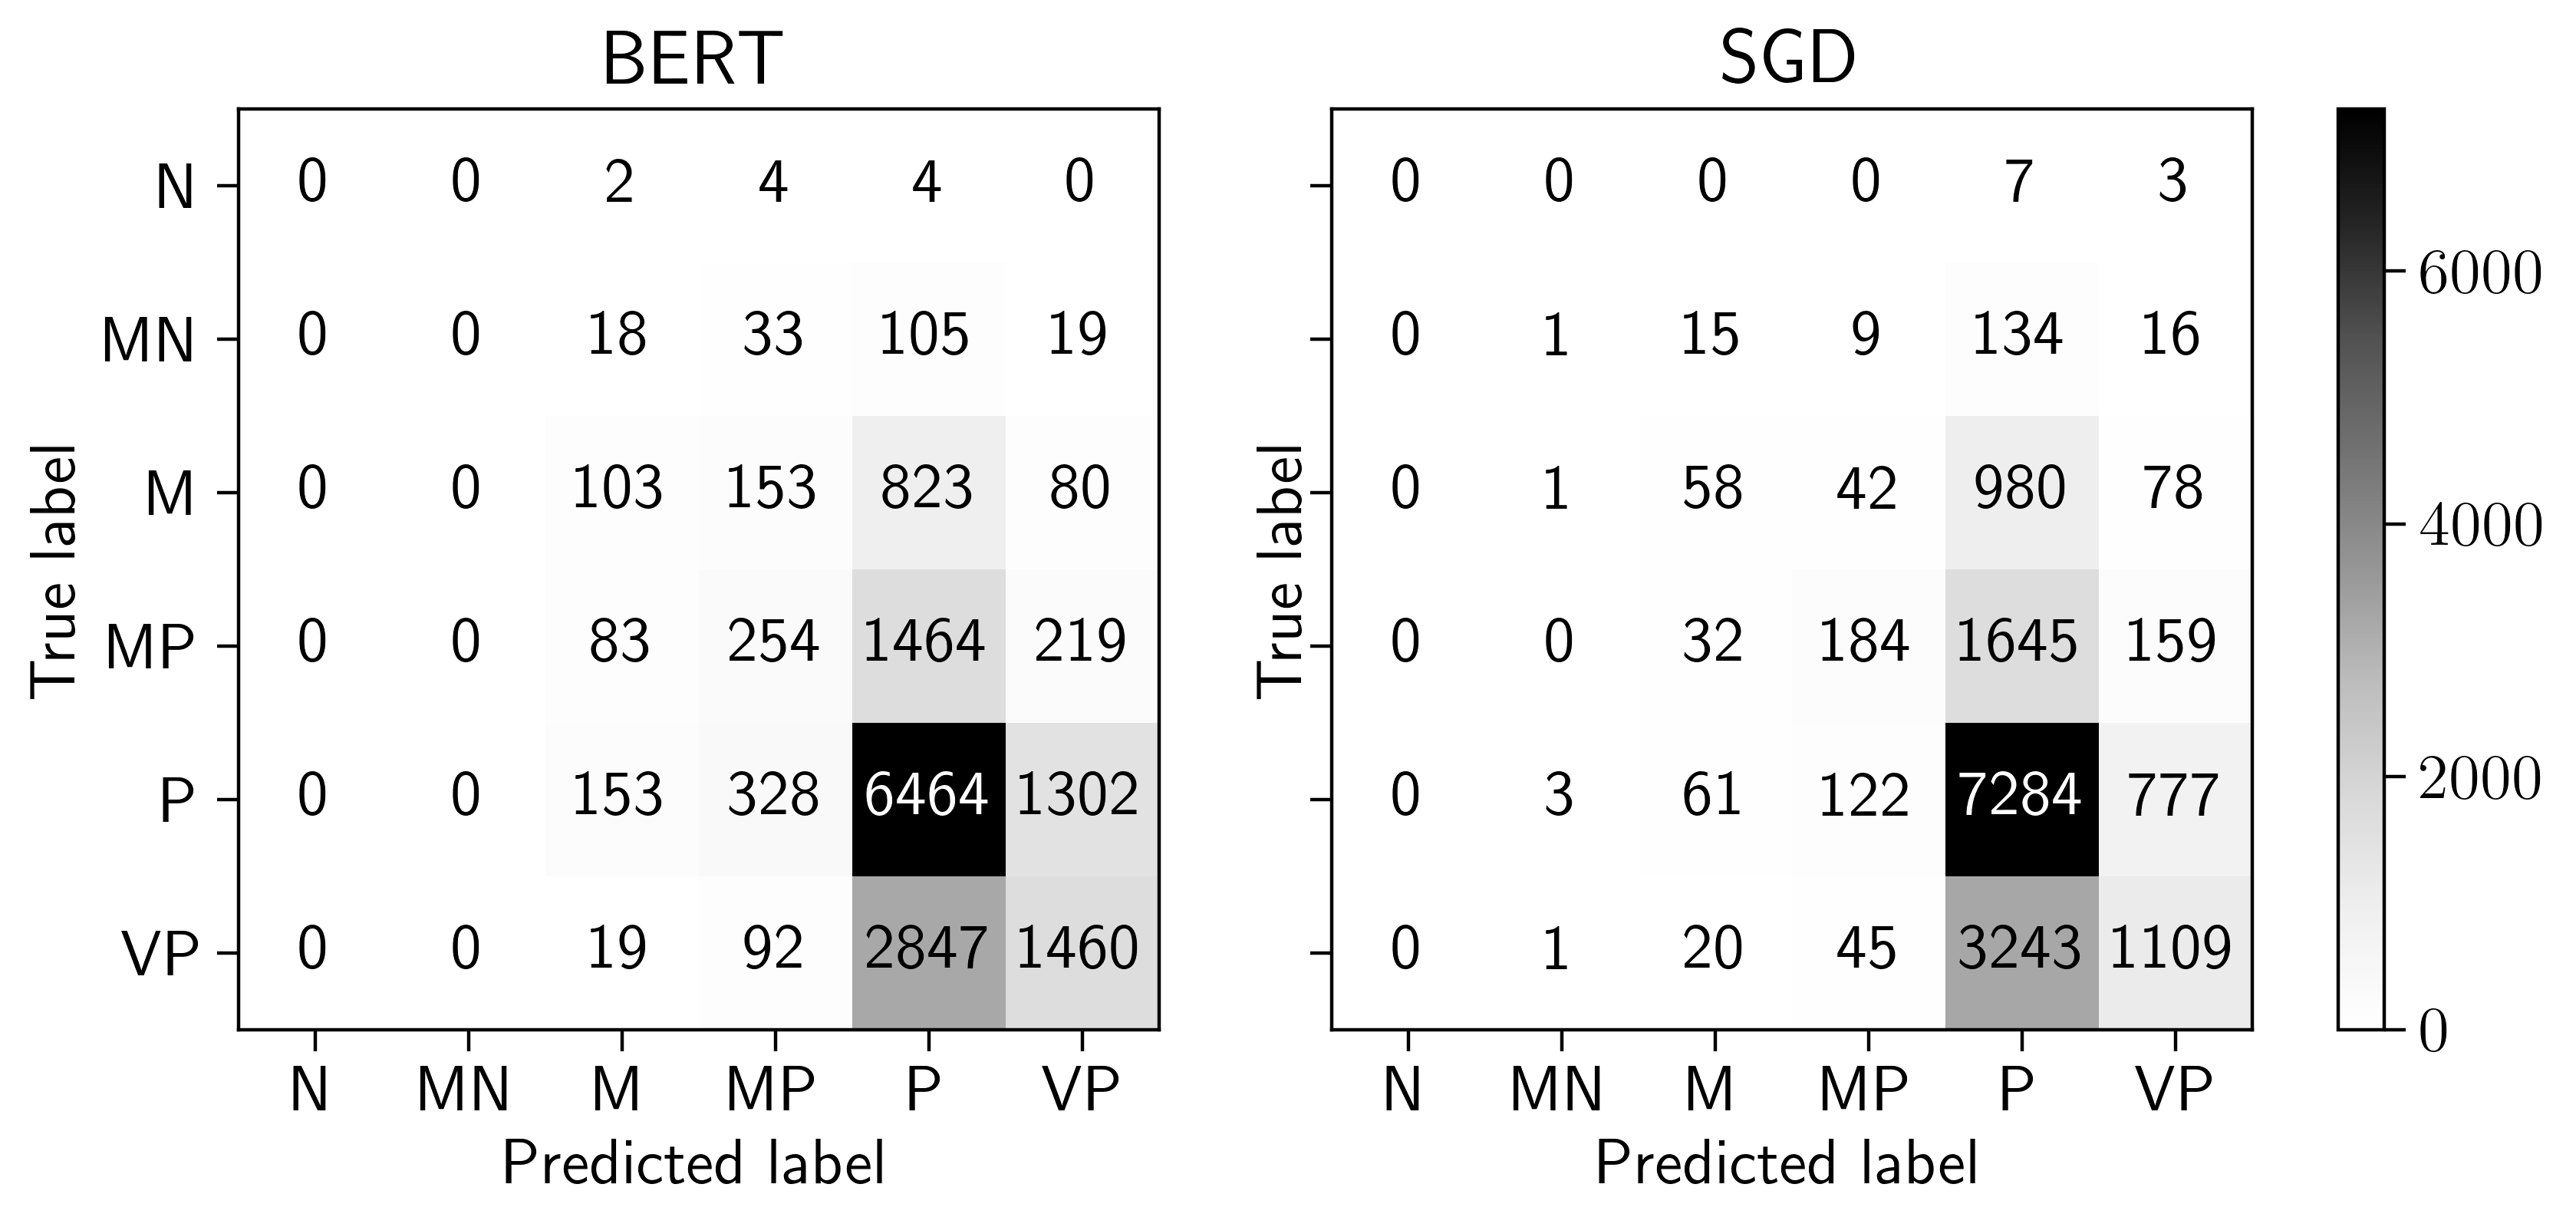
\includegraphics[width=0.85\textwidth]{figures/06_results/02_pu/01_cm/any_6.png}
    \caption{Confusion matrices for 6-class, multilingual sample.}
    \label{fig:Res_PU_CM_M6}
\end{figure}

The primary difference between the classifications made by the English and multilingual models appears to be in the frequency with which the `positive' label is predicted. The multilingual models tend to mislabel `very positive', `mostly positive' and `mixed' reviews as `positive' more often than the English models do. This characteristic seems to be the main reason behind their poorer performances.

\paragraph{Three Rating Classes}

Confusion matrices for the 3-class, English and multilingual samples can be seen in Figures \ref{fig:Res_PU_CM_E3} and \ref{fig:Res_PU_CM_M3}, respectively.

\begin{figure}[ht]
    \centering
    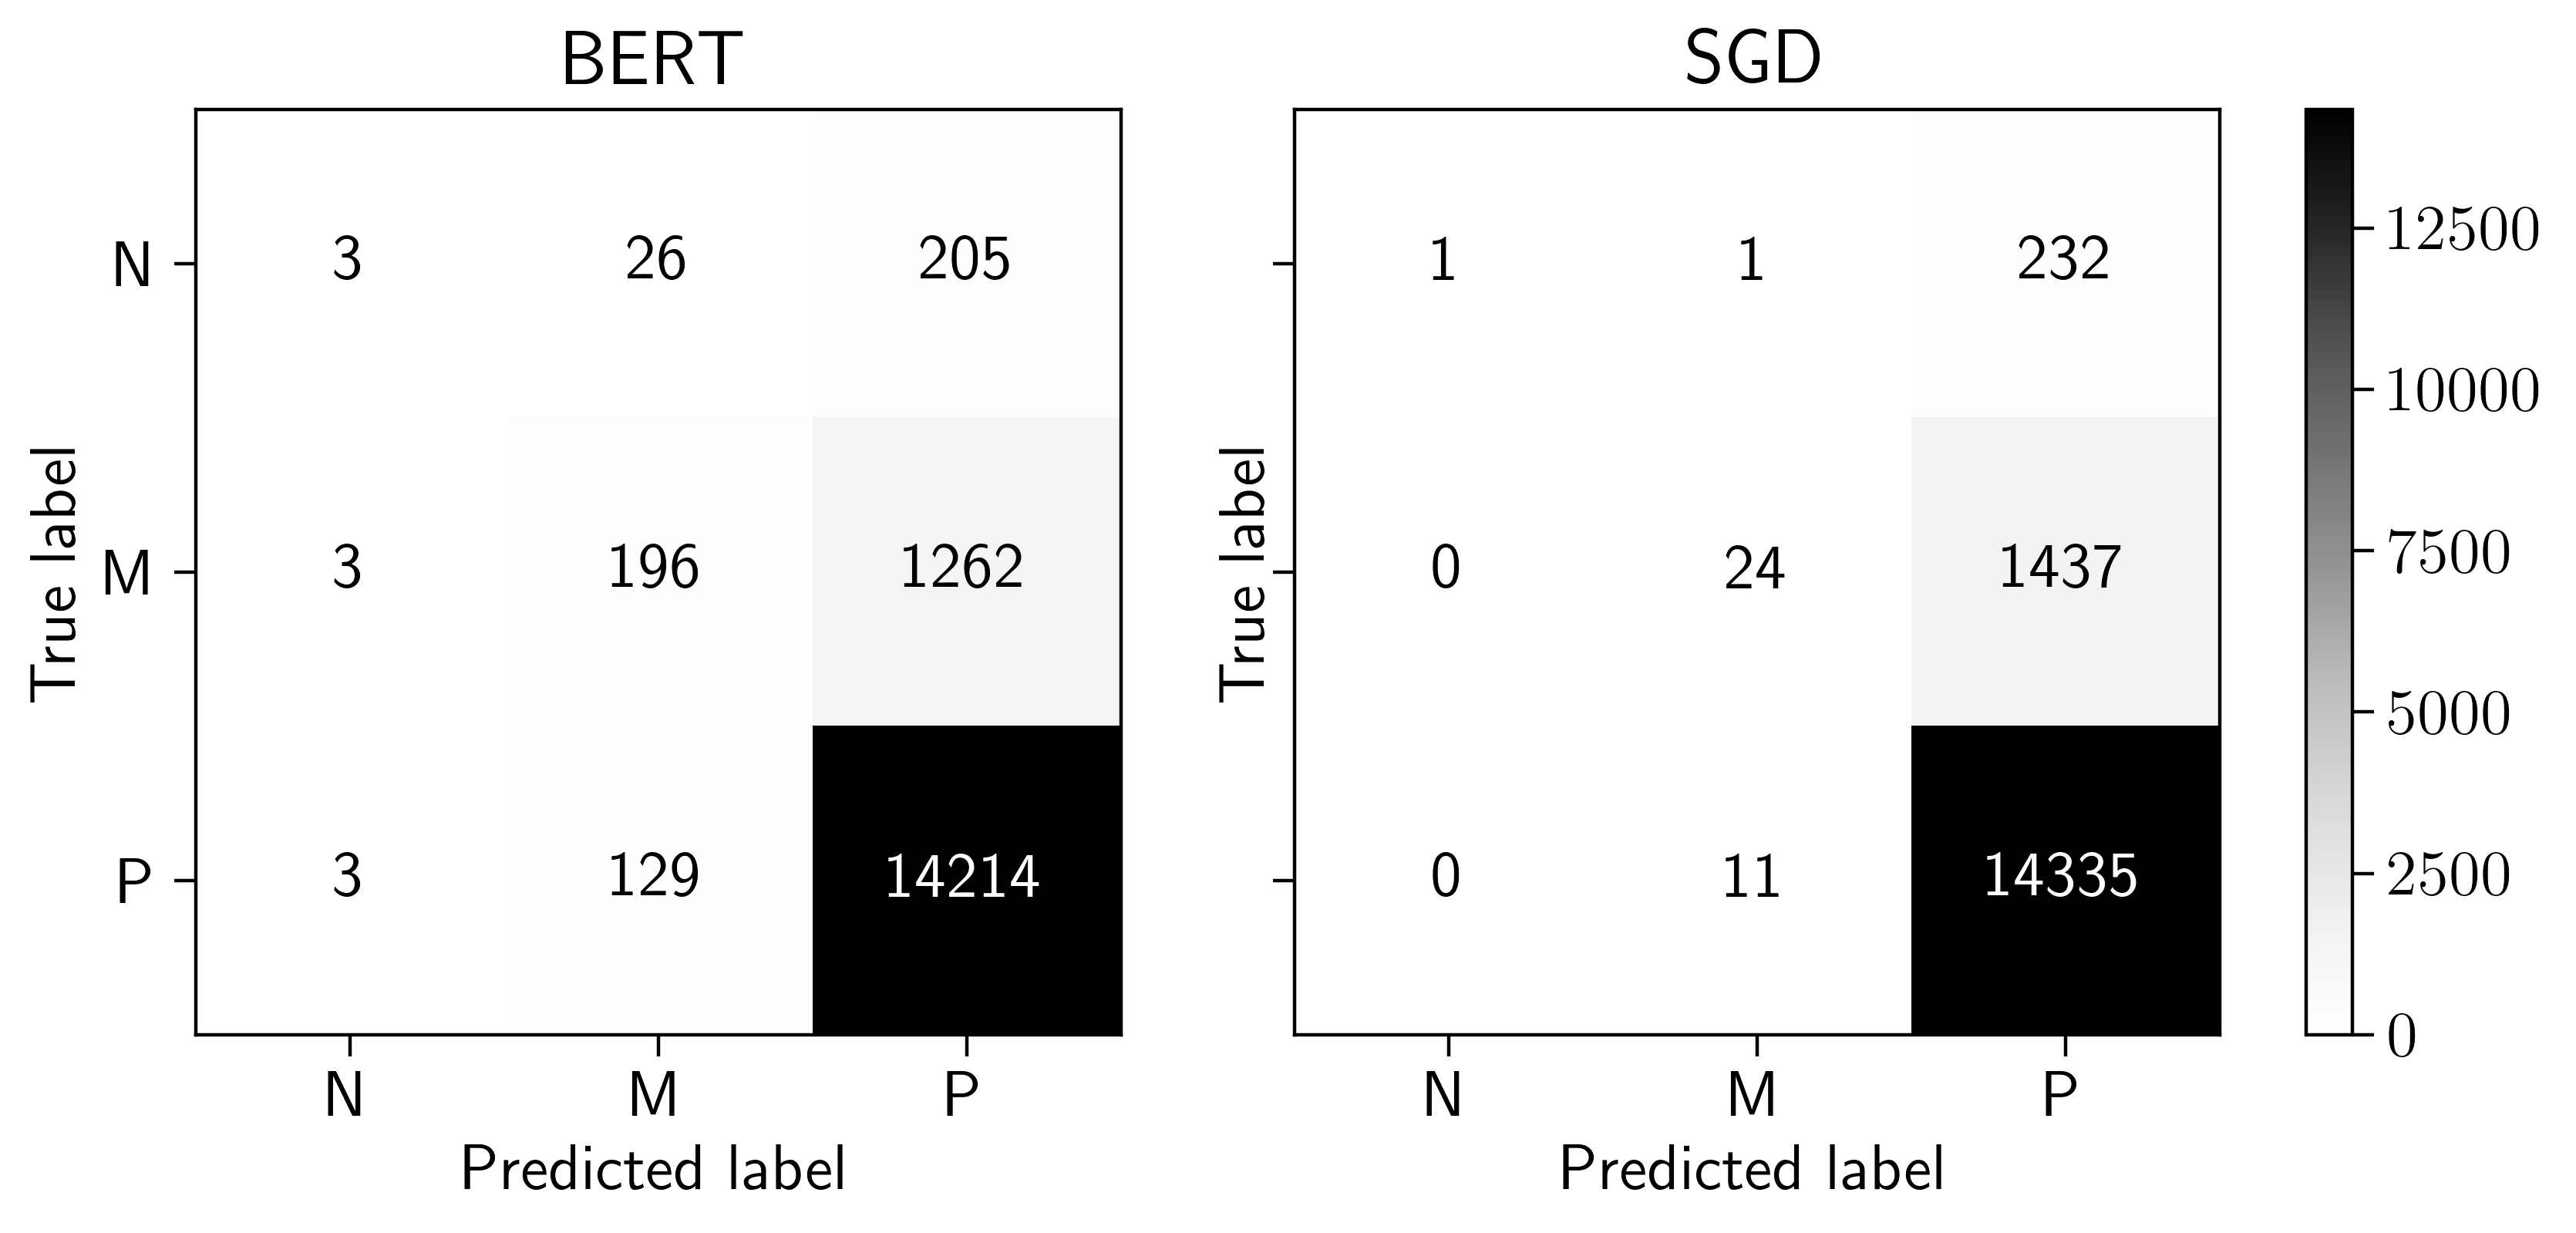
\includegraphics[width=0.85\textwidth]{figures/06_results/02_pu/01_cm/eng_3.png}
    \caption{Confusion matrices for 3-class, English sample.}
    \label{fig:Res_PU_CM_E3}
\end{figure}

\begin{figure}[ht]
    \centering
    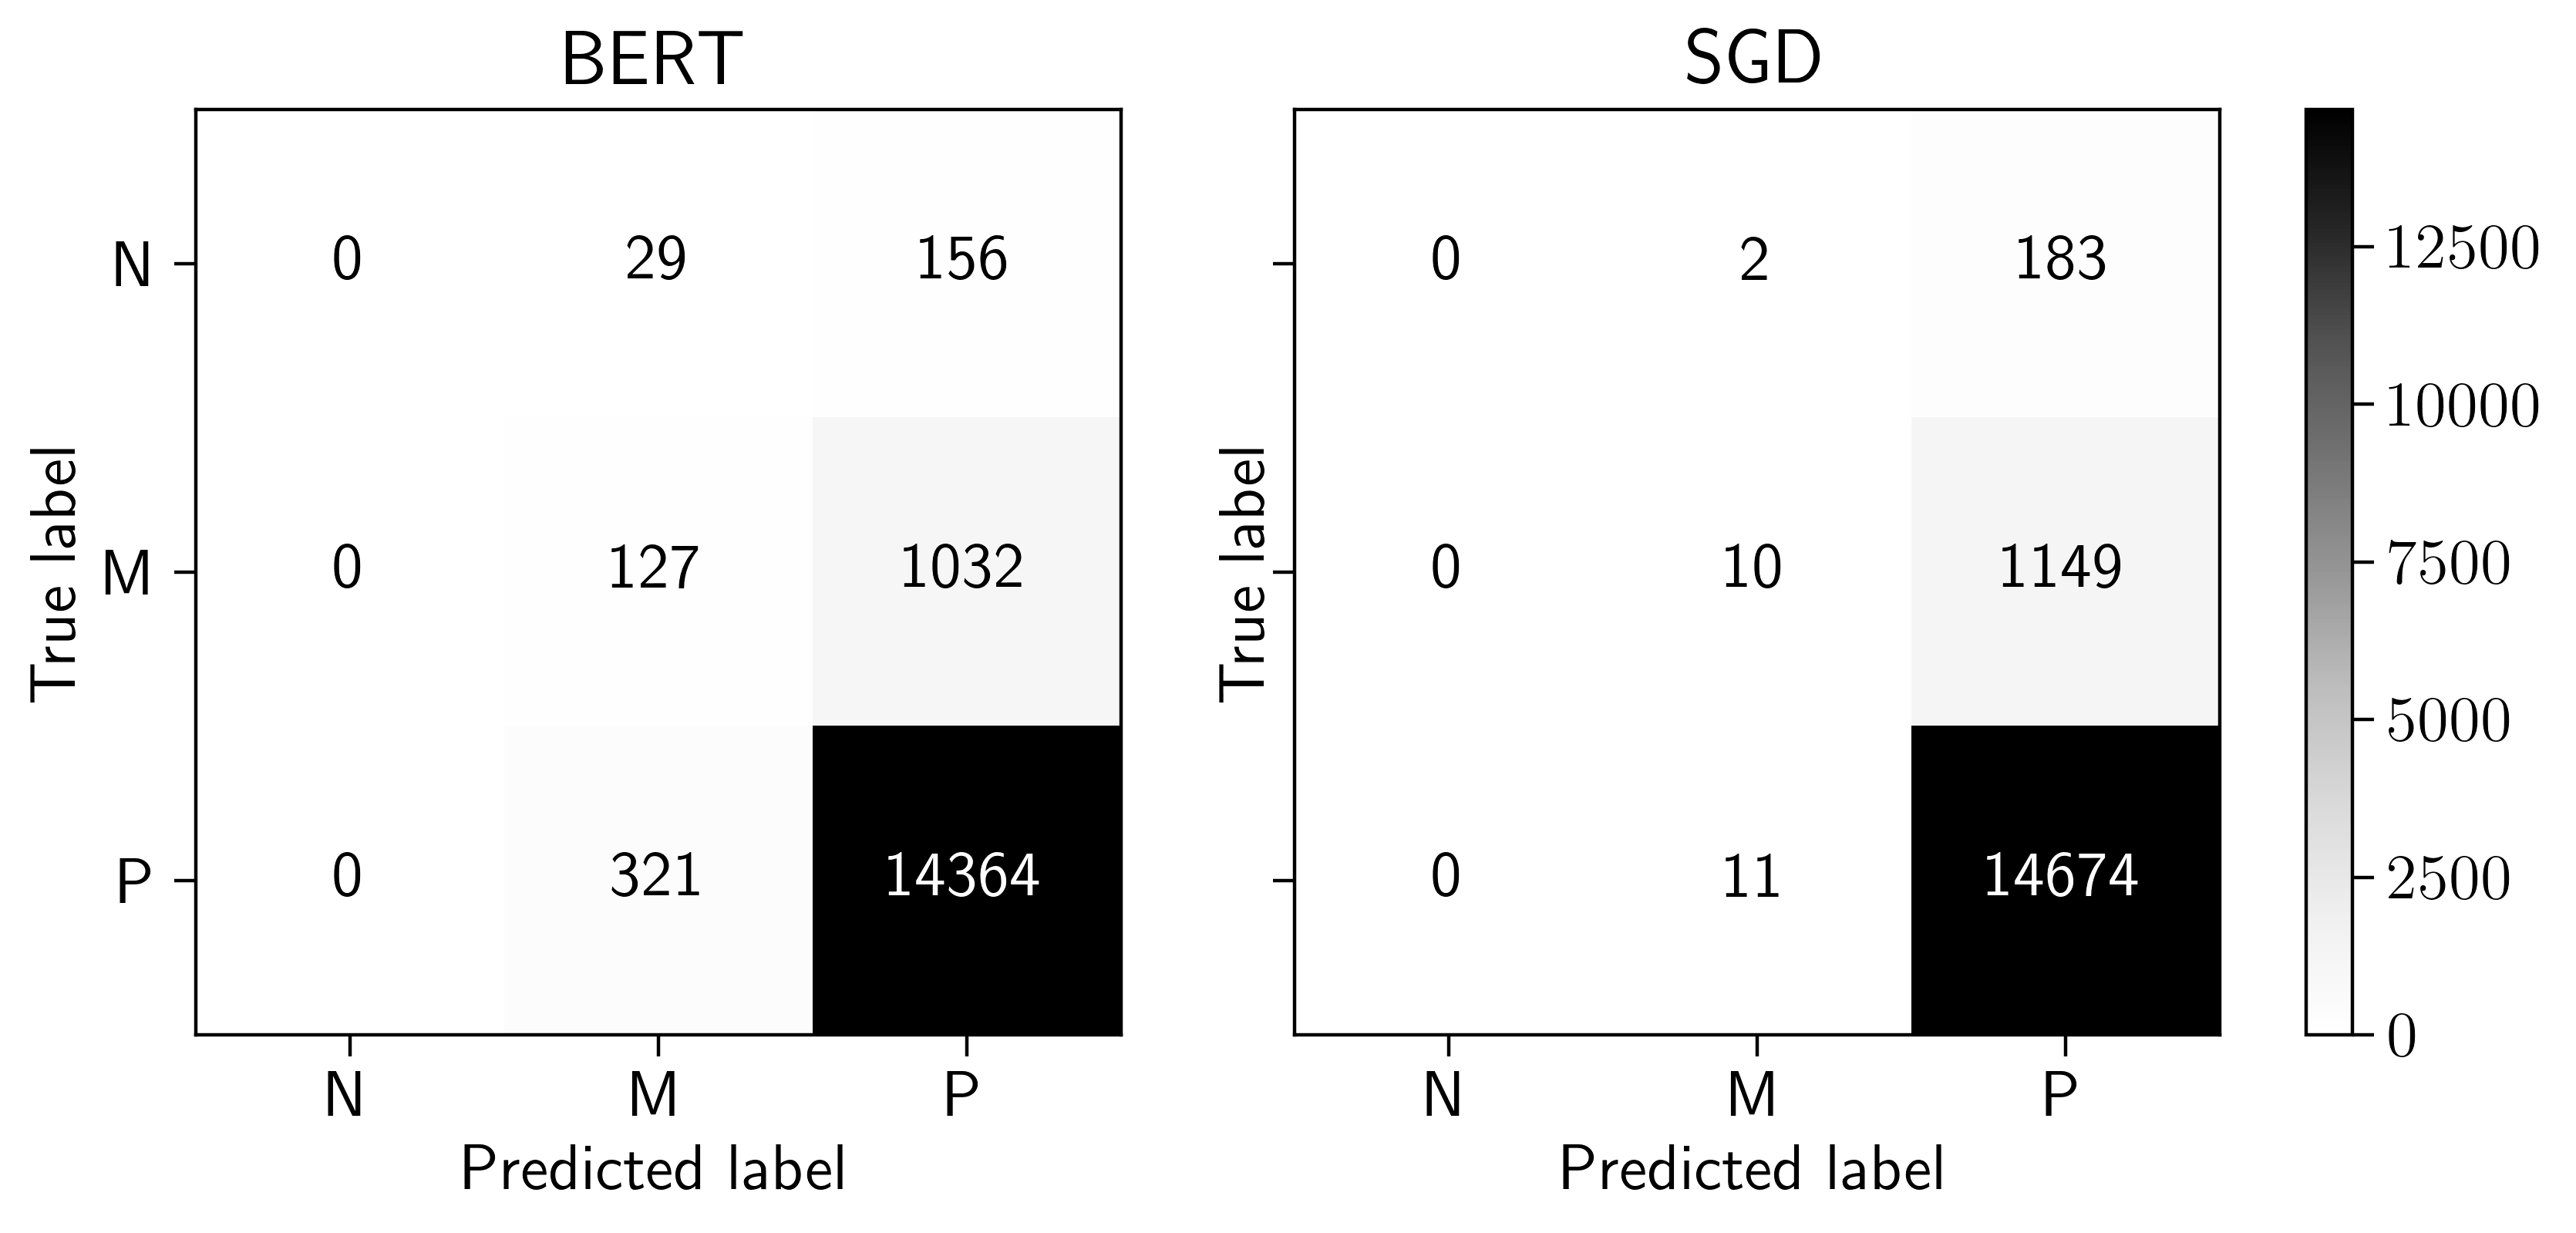
\includegraphics[width=0.85\textwidth]{figures/06_results/02_pu/01_cm/any_3.png}
    \caption{Confusion matrices for 3-class, multilingual sample.}
    \label{fig:Res_PU_CM_M3}
\end{figure}

All of the 3-class models tend to make solely `positive' predictions. The BERT models do occasionally predict the `mixed' label, although these predictions appear to be mostly incorrect, leading to predictive accuracies which are worse than their respective baselines.

\subsection{User-based Results}

In this section, the trained models will be assessed on a per-user basis. Instead of considering the overall accuracy or performance of the models when evaluated against the entire test set, the proportions of users whose review classes are accurately modelled by the classifiers, relative to various baselines, will be examined and compared.

\subsubsection{User Accuracy}

The accuracies of the users in each sample will be compared in this section. For each user, the percentage of their reviews which were accurately classified by each model - BF, BERT and SGD - will be calculated. The calculated accuracies will be plotted in the form of a reverse cumulative distribution function which will show, for any accuracy $x$, what percentage of the users in the test set have had their reviews predicted with an accuracy of at least $x$. For example, 100\% of users will have an accuracy of at least 0\%, while only a very small number of users will have an accuracy of 100\%.

\paragraph{Six Rating Classes}

The user accuracy distributions for the BF, BERT and SGD models against the 6-class samples can be seen in Figure \ref{fig:Res_PU_Simp_6}.

\begin{figure}[ht]
    \centering
    \begin{subfigure}[ht]{0.49\textwidth}
        \centering
        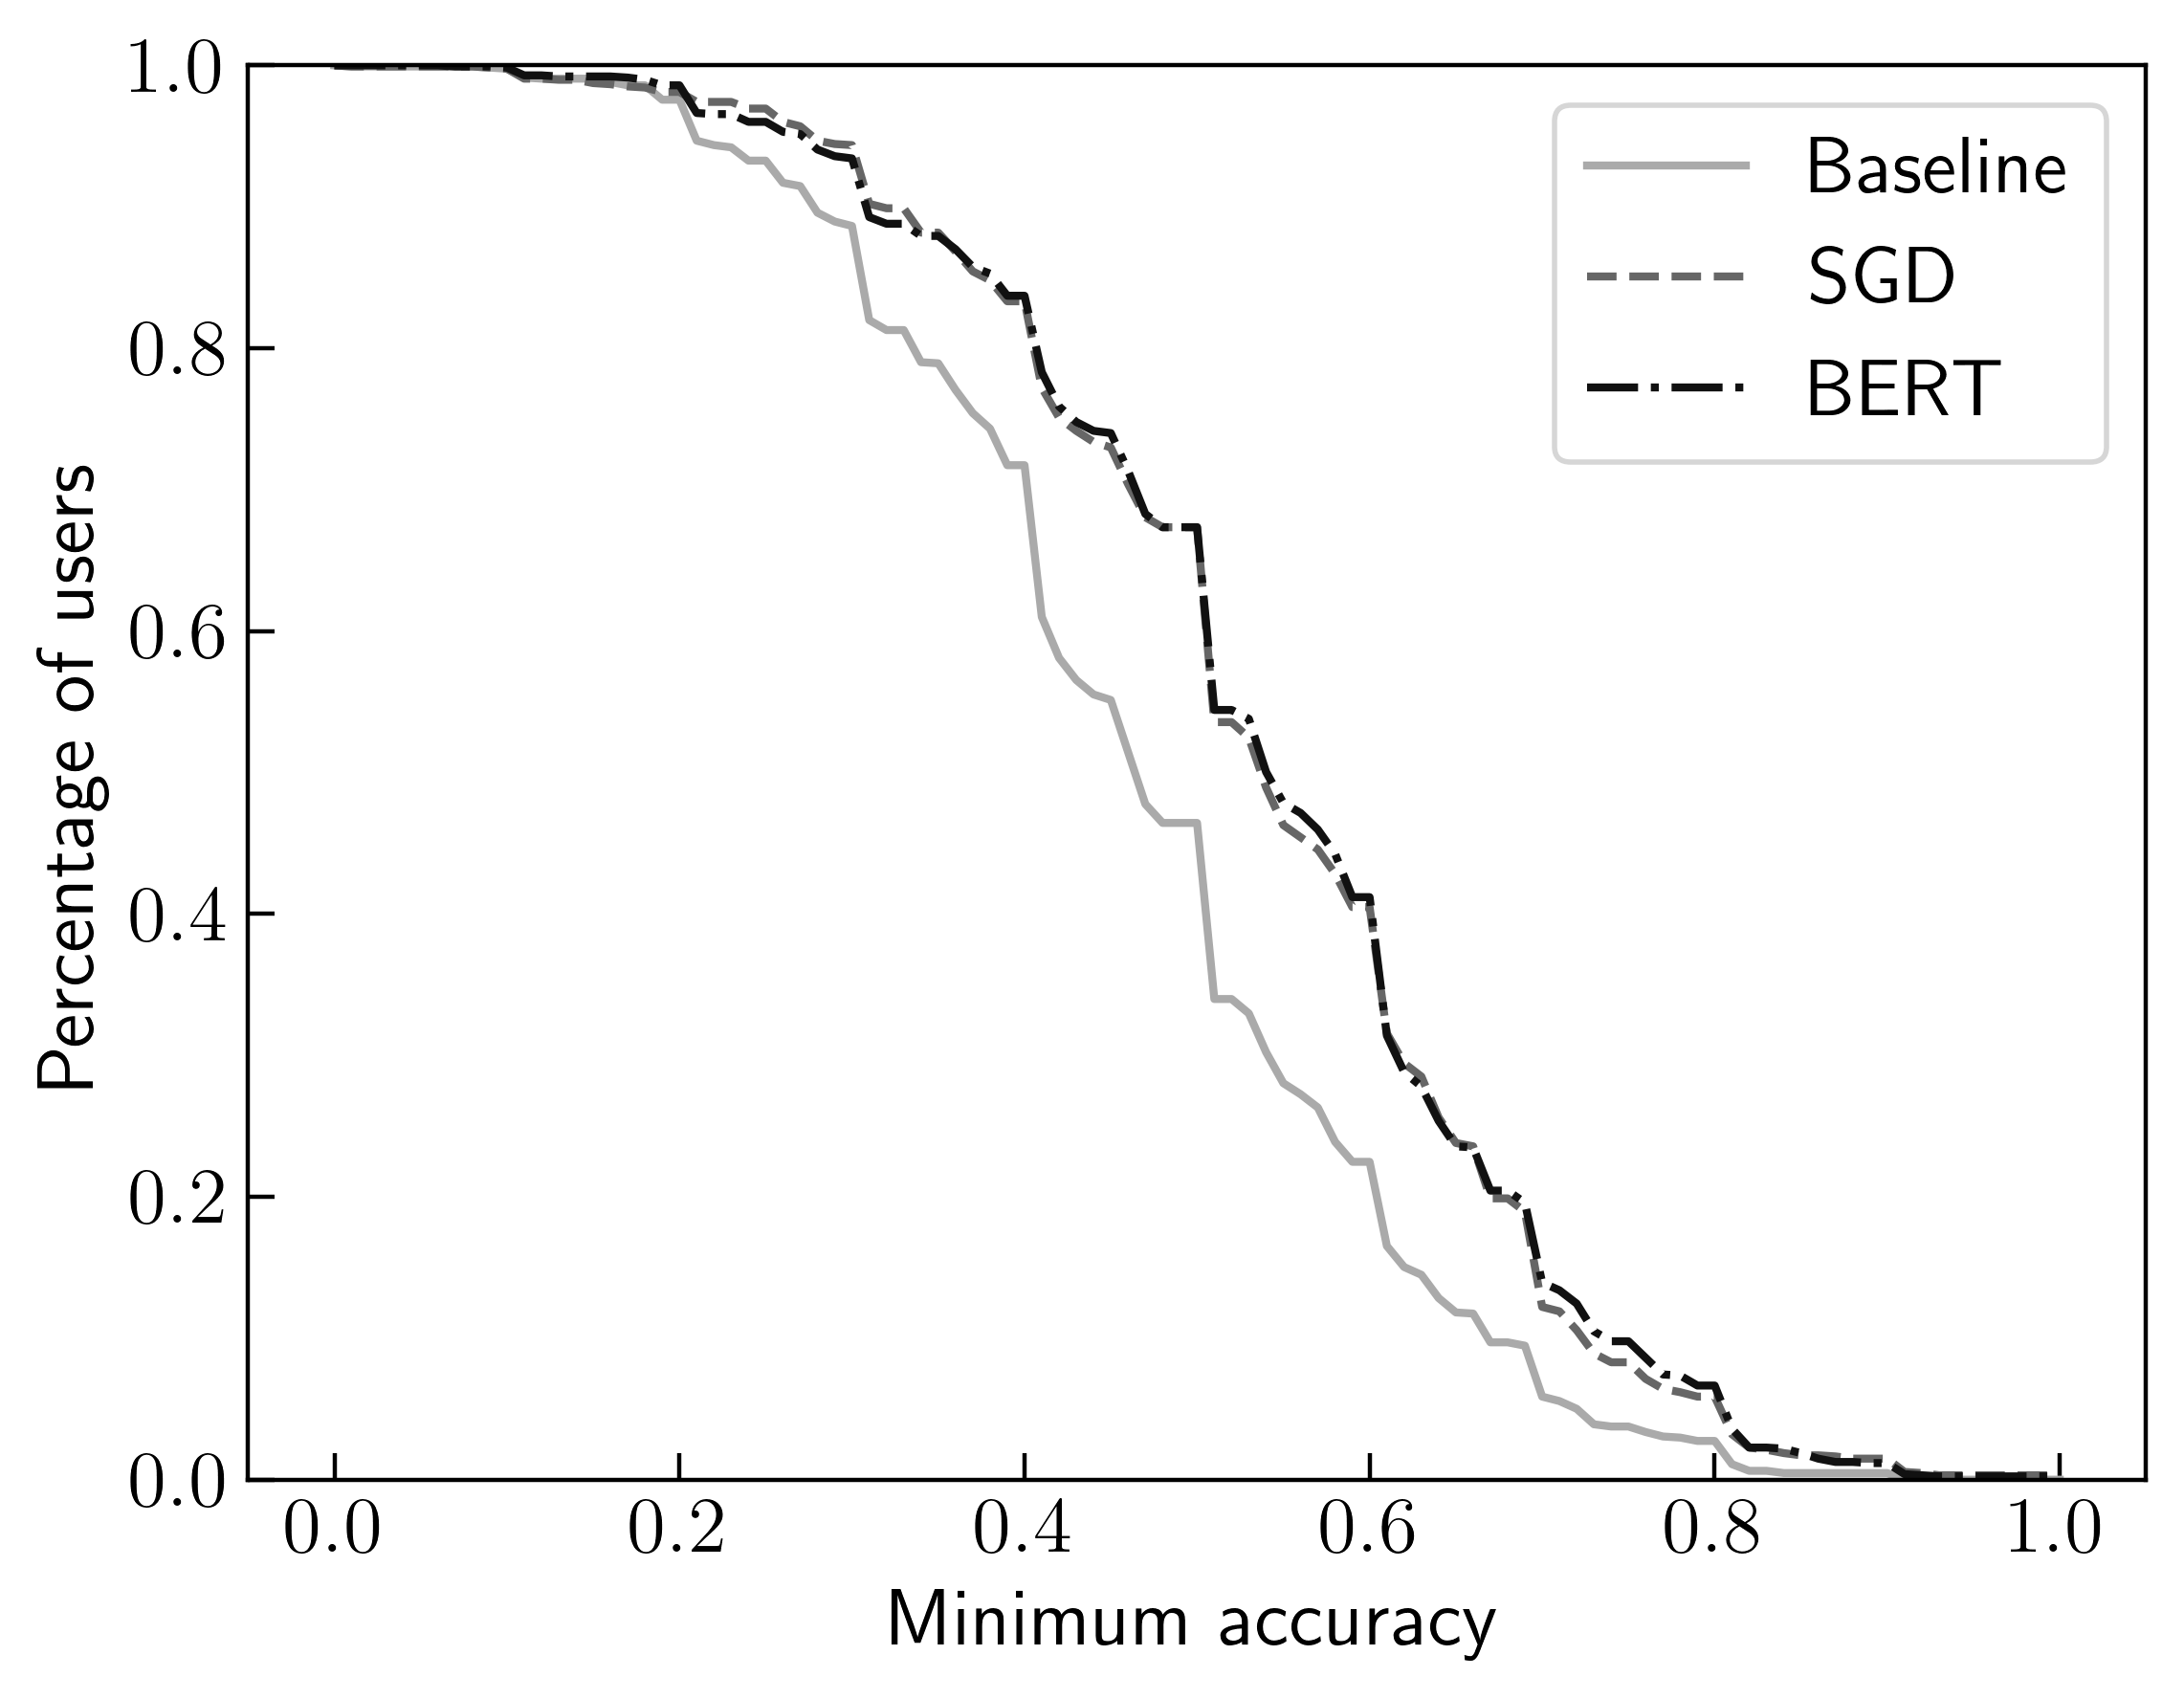
\includegraphics[width=\textwidth]{figures/06_results/02_pu/02_simple/eng_6.png}
        \caption{English.}
        \label{fig:Res_PU_Simp_E6}
    \end{subfigure}
    \hfill
    \begin{subfigure}[ht]{0.49\textwidth}
        \centering
        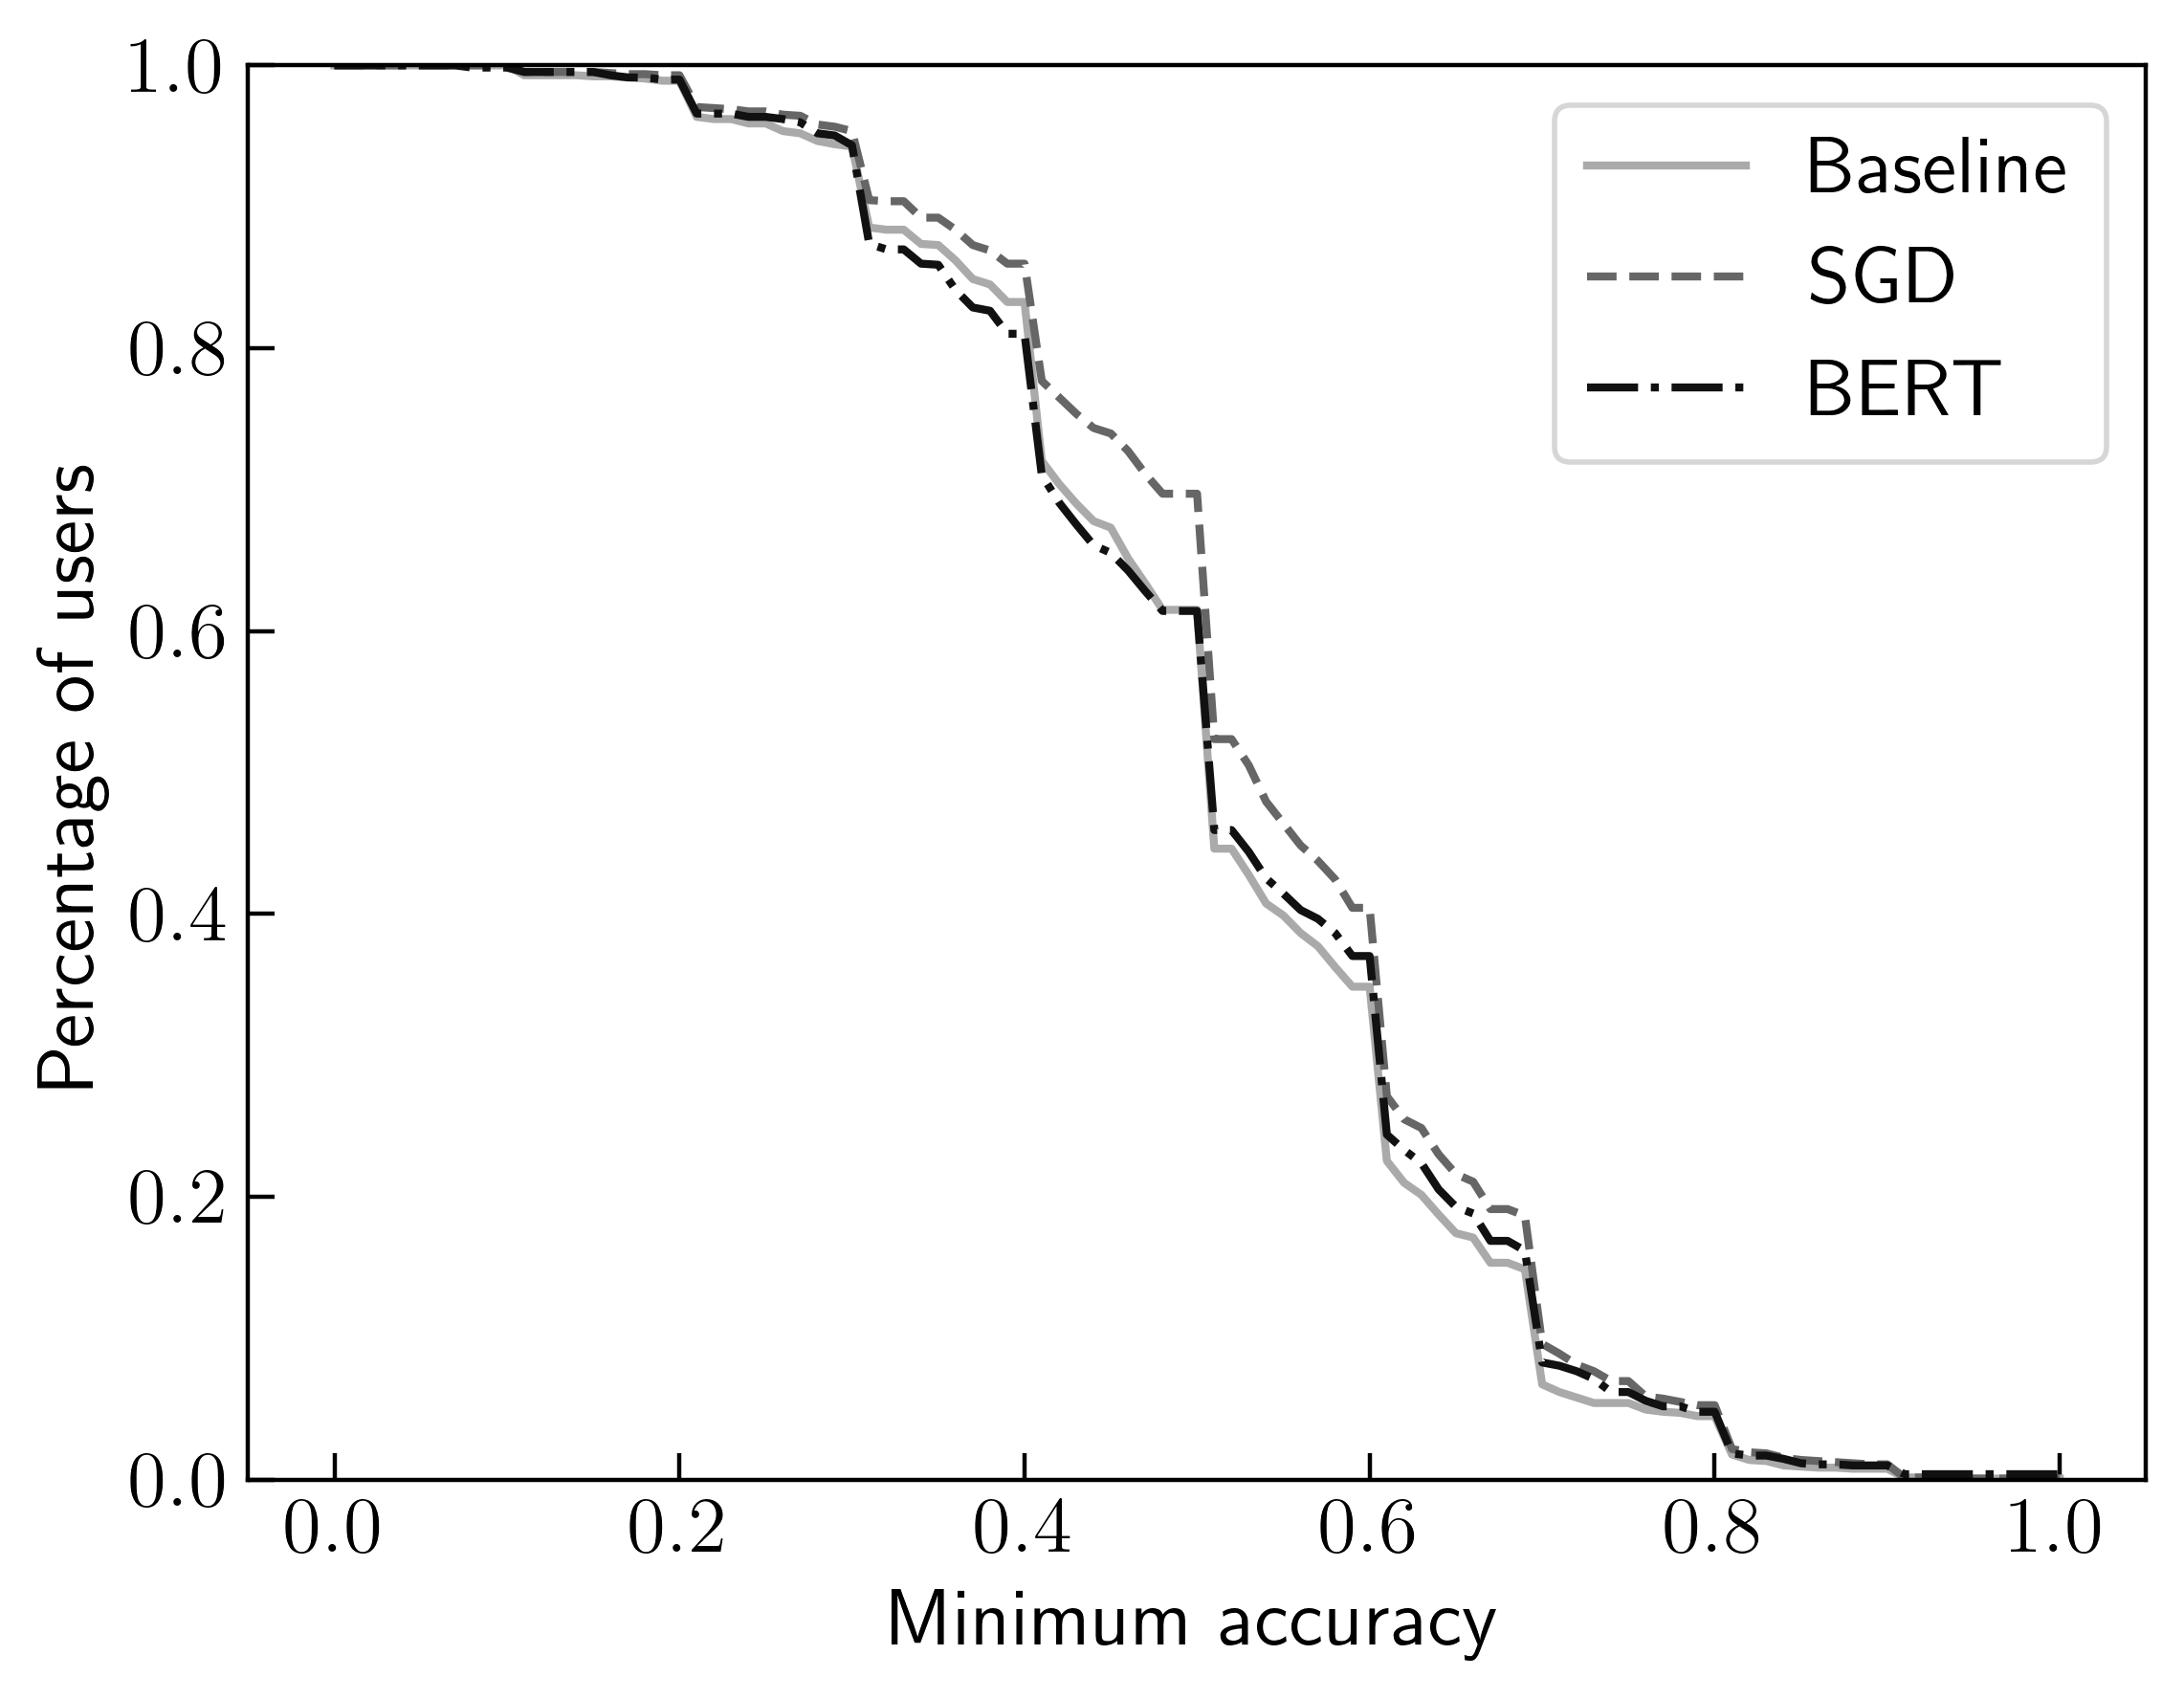
\includegraphics[width=\textwidth]{figures/06_results/02_pu/02_simple/any_6.png}
        \caption{Multilingual.}
        \label{fig:Res_PU_Simp_M6}
    \end{subfigure}
    \caption{User accuracy distribution for 6-class samples.}
    \label{fig:Res_PU_Simp_6}
\end{figure}

For the English sample, the superior performances of both the BERT and SGD models, relative to the BF model, are clearly displayed. The trained models consistently classify individual users more accurately than the baseline at all non-extreme minimum accuracies, ie between 10\% and 90\%. At certain points, the absolute difference between the trained models and the baseline is greater than 20\%.

For the multilingual sample, the performances of the trained models and the baseline are quite similar. The BERT and BF models produce almost identical results and, although the SGD model does appear to be slightly more accurate at times, the difference is nowhere near as pronounced as it was for the English sample.

\paragraph{Three Rating Classes}

The user accuracy distributions for the BF, BERT and SGD models and the 3-class samples can be seen in Figure \ref{fig:Res_PU_Simp_3}.

\begin{figure}[ht]
    \centering
    \begin{subfigure}[ht]{0.49\textwidth}
        \centering
        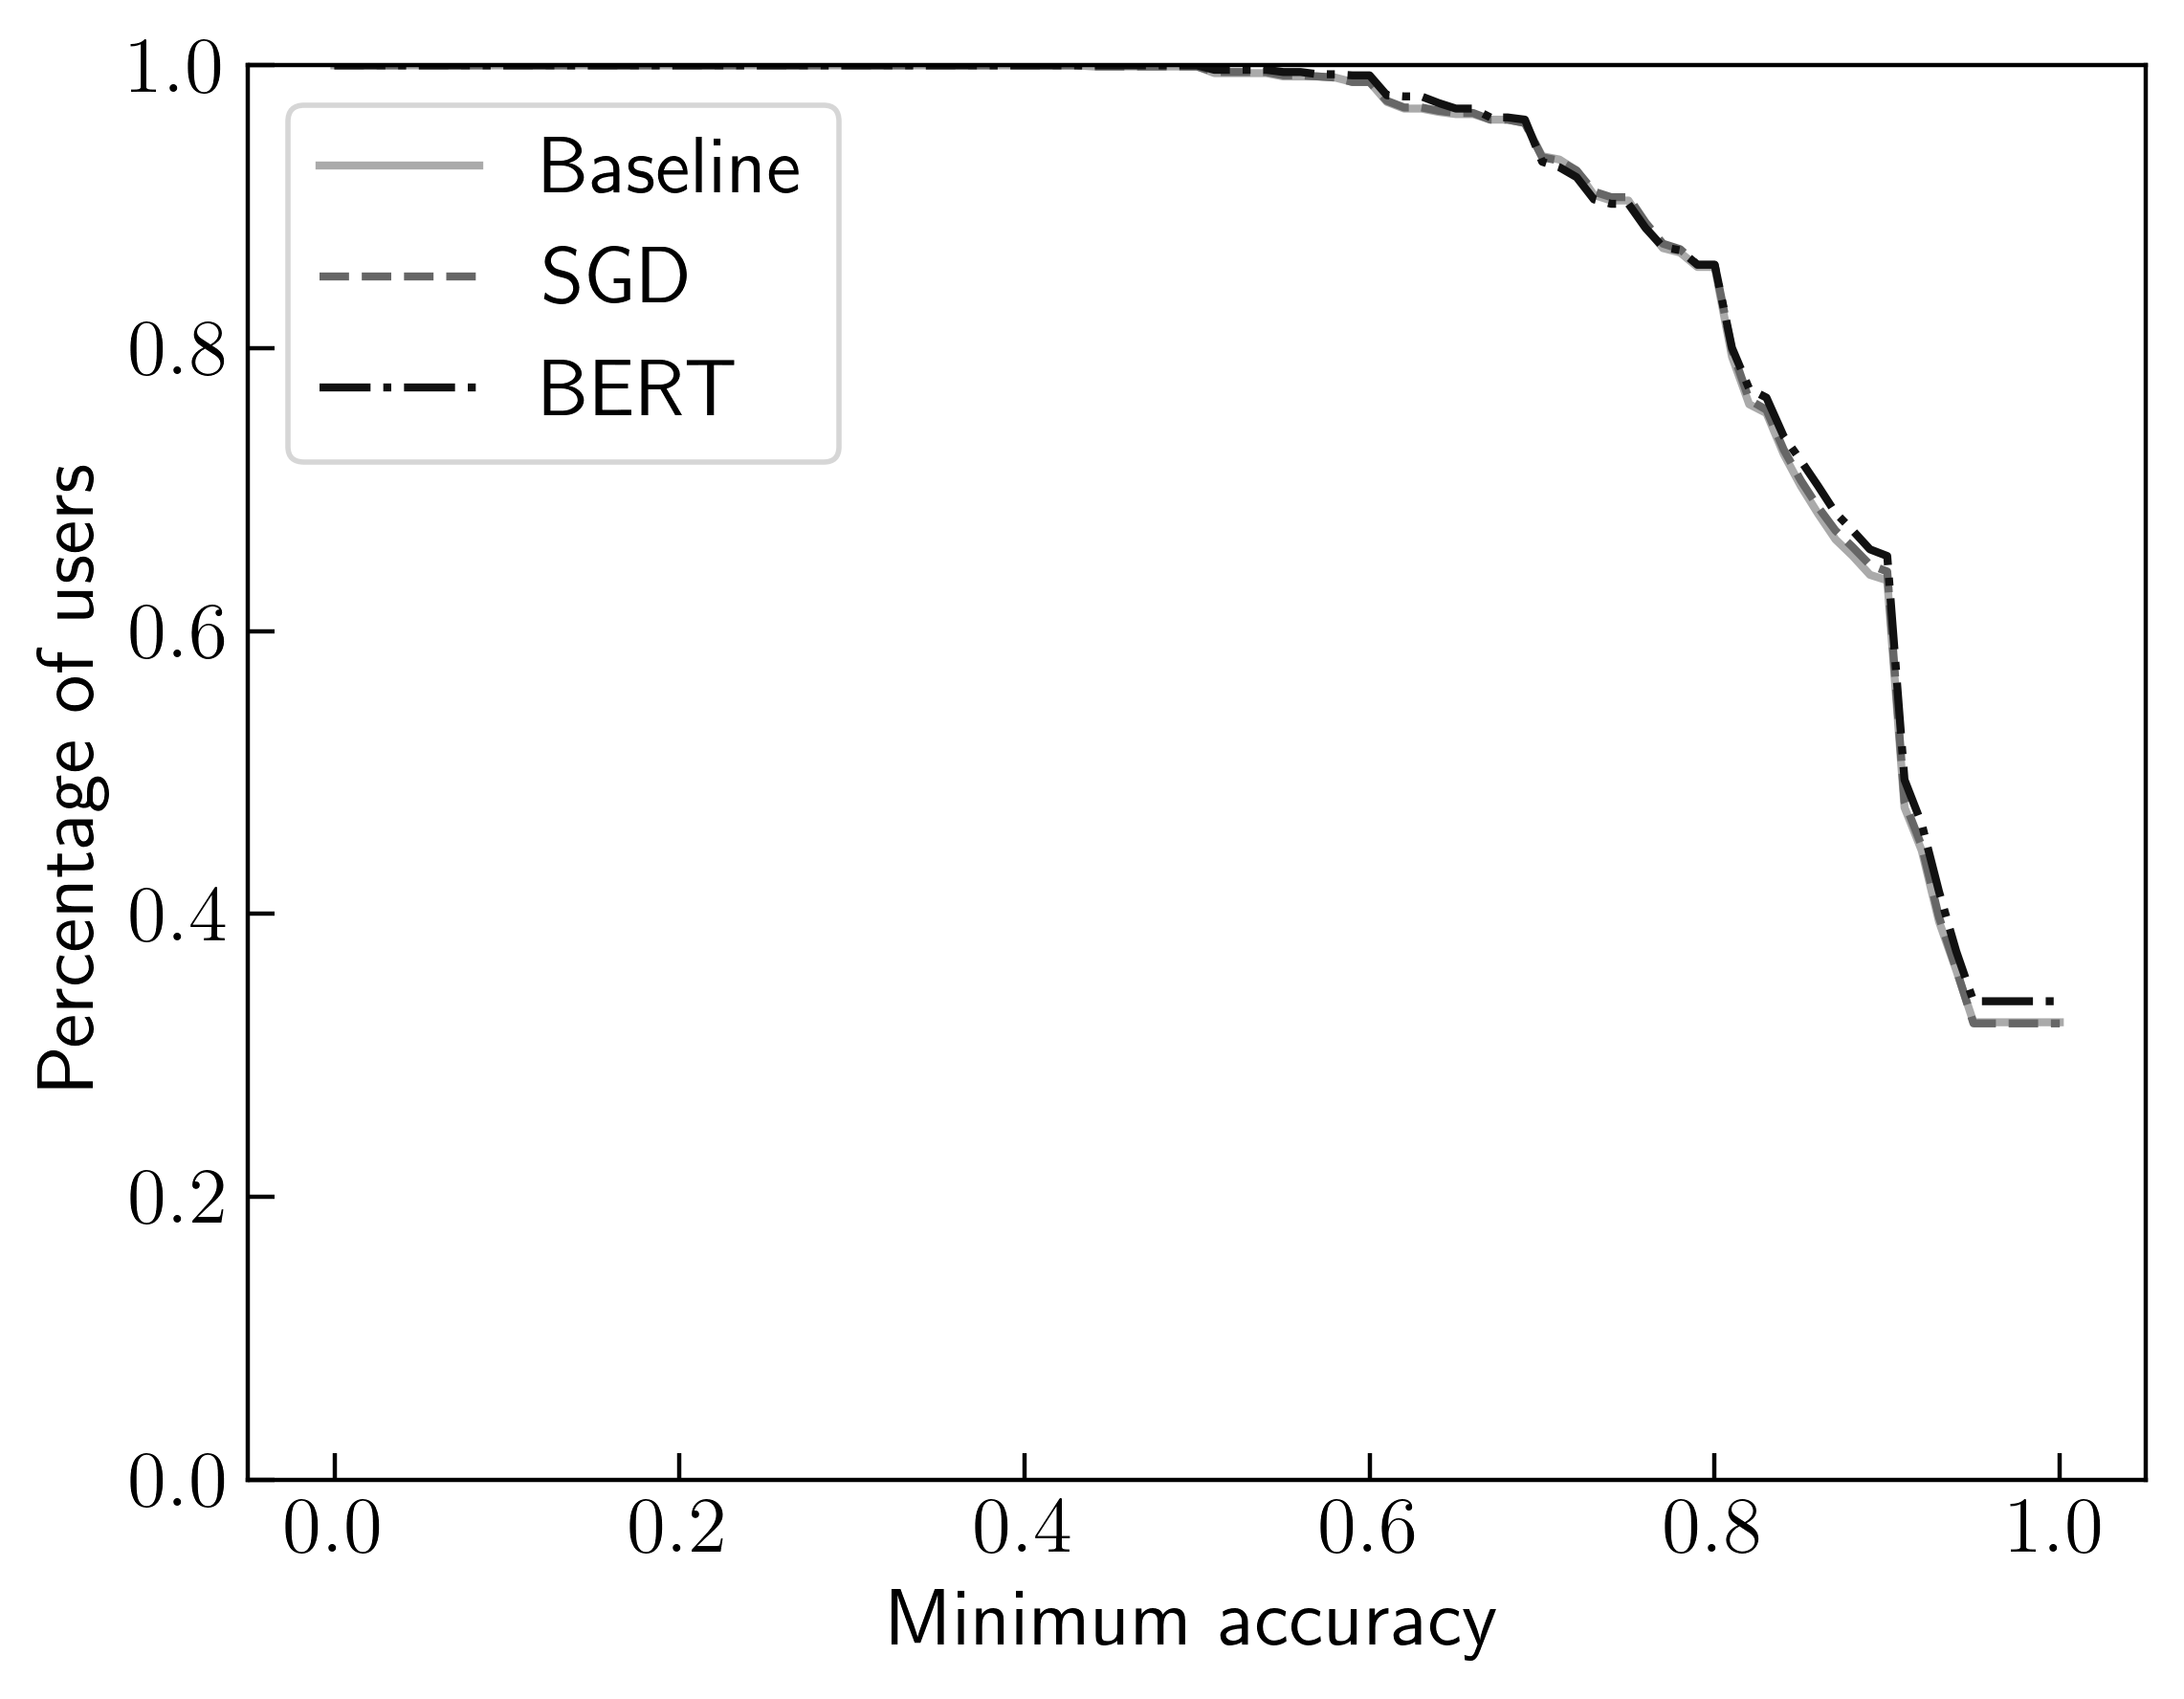
\includegraphics[width=\textwidth]{figures/06_results/02_pu/02_simple/eng_3.png}
        \caption{English.}
        \label{fig:Res_PU_Simp_E3}
    \end{subfigure}
    \hfill
    \begin{subfigure}[ht]{0.49\textwidth}
        \centering
        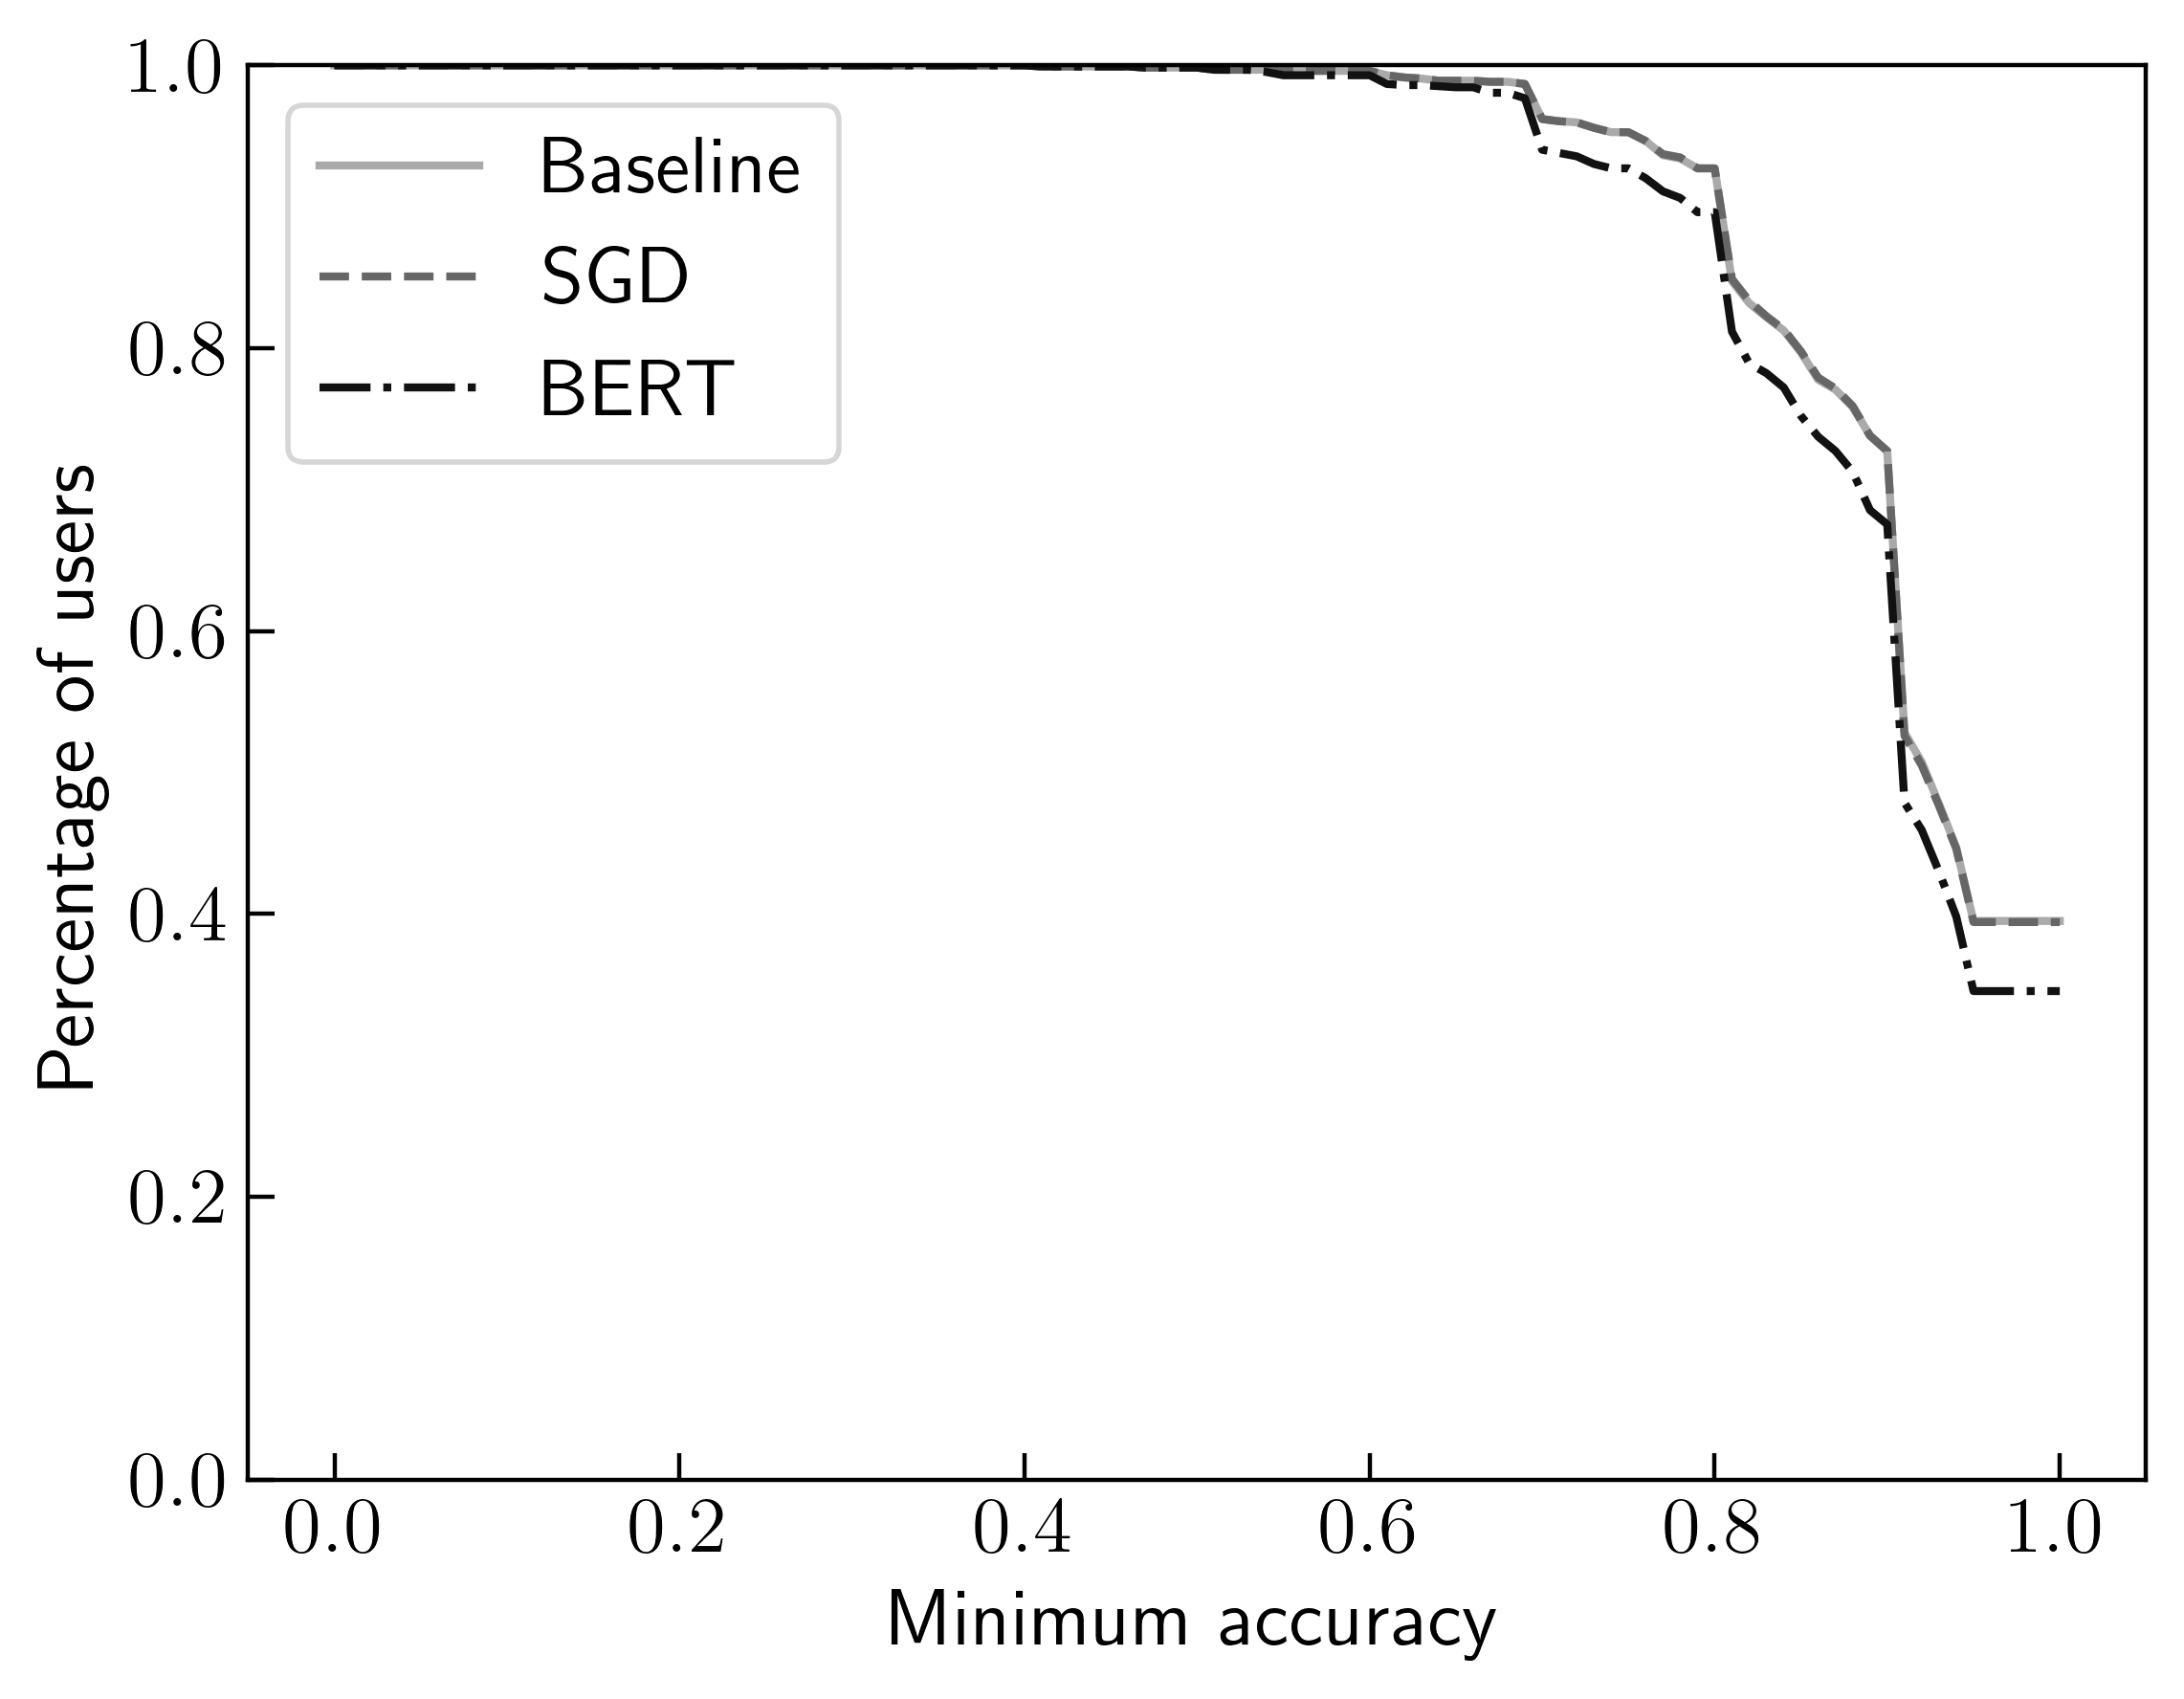
\includegraphics[width=\textwidth]{figures/06_results/02_pu/02_simple/any_3.png}
        \caption{Multilingual.}
        \label{fig:Res_PU_Simp_M3}
    \end{subfigure}
    \caption{User accuracy distribution for 3-class samples.}
    \label{fig:Res_PU_Simp_3}
\end{figure}

For both of the samples, the user accuracy distributions do not appear to be of any use. Because of the imbalanced distribution of labels and, due to the review inclusion criteria outlined in section \ref{sec:DI_RU}, over 30\% of users have only written reviews for games that were labelled `positive'. This has resulted in the baseline classifier having a 100\% accuracy rate for more than a third of all users in the sample. This effect, combined with the inability of the trained models to outperform the baseline, means that further investigation into the determination of representative users using the 3-class samples is pointless.

\subsubsection{Percentile Selection Method}

By using the user accuracy distributions, the users whose reviews, according to the trained models, are most representative of the games' average ratings can be determined. Percentiles could be employed to select the representative users. For example, only the most accurate 10\% of users, ie users in the 90\textsuperscript{th} percentile, might be considered.

This selection criterion, relying solely on accuracy percentiles, would include users with a high baseline accuracy, too. For example, a user who only reviewed games that were labelled `positive' would receive a practically meaningless baseline accuracy of 100\%. A more precise selection criterion would only consider users whose BERT or SGD accuracy was, for instance, at least 20\% larger than their baseline accuracy. This method would also limit the potential pool of representative users to those who had reviewed games of various rating classes, or at very least, those who had not solely reviewed `positive' games. A potential drawback of this more precise selection method is that genuinely representative users who happened to only/mostly review `positive' games would also be excluded.

An example of this method, indicating the minimum user accuracies required to be in the 80\textsuperscript{th}, 90\textsuperscript{th}, 95\textsuperscript{th} and 99\textsuperscript{th} percentiles, for both the BERT and SGD models, can be found in Figure \ref{fig:Res_PU_PctsExample}. It considers only those users whose trained model accuracies were at least 20\% larger than their baseline accuracy.

\begin{figure}[ht]
    \centering
    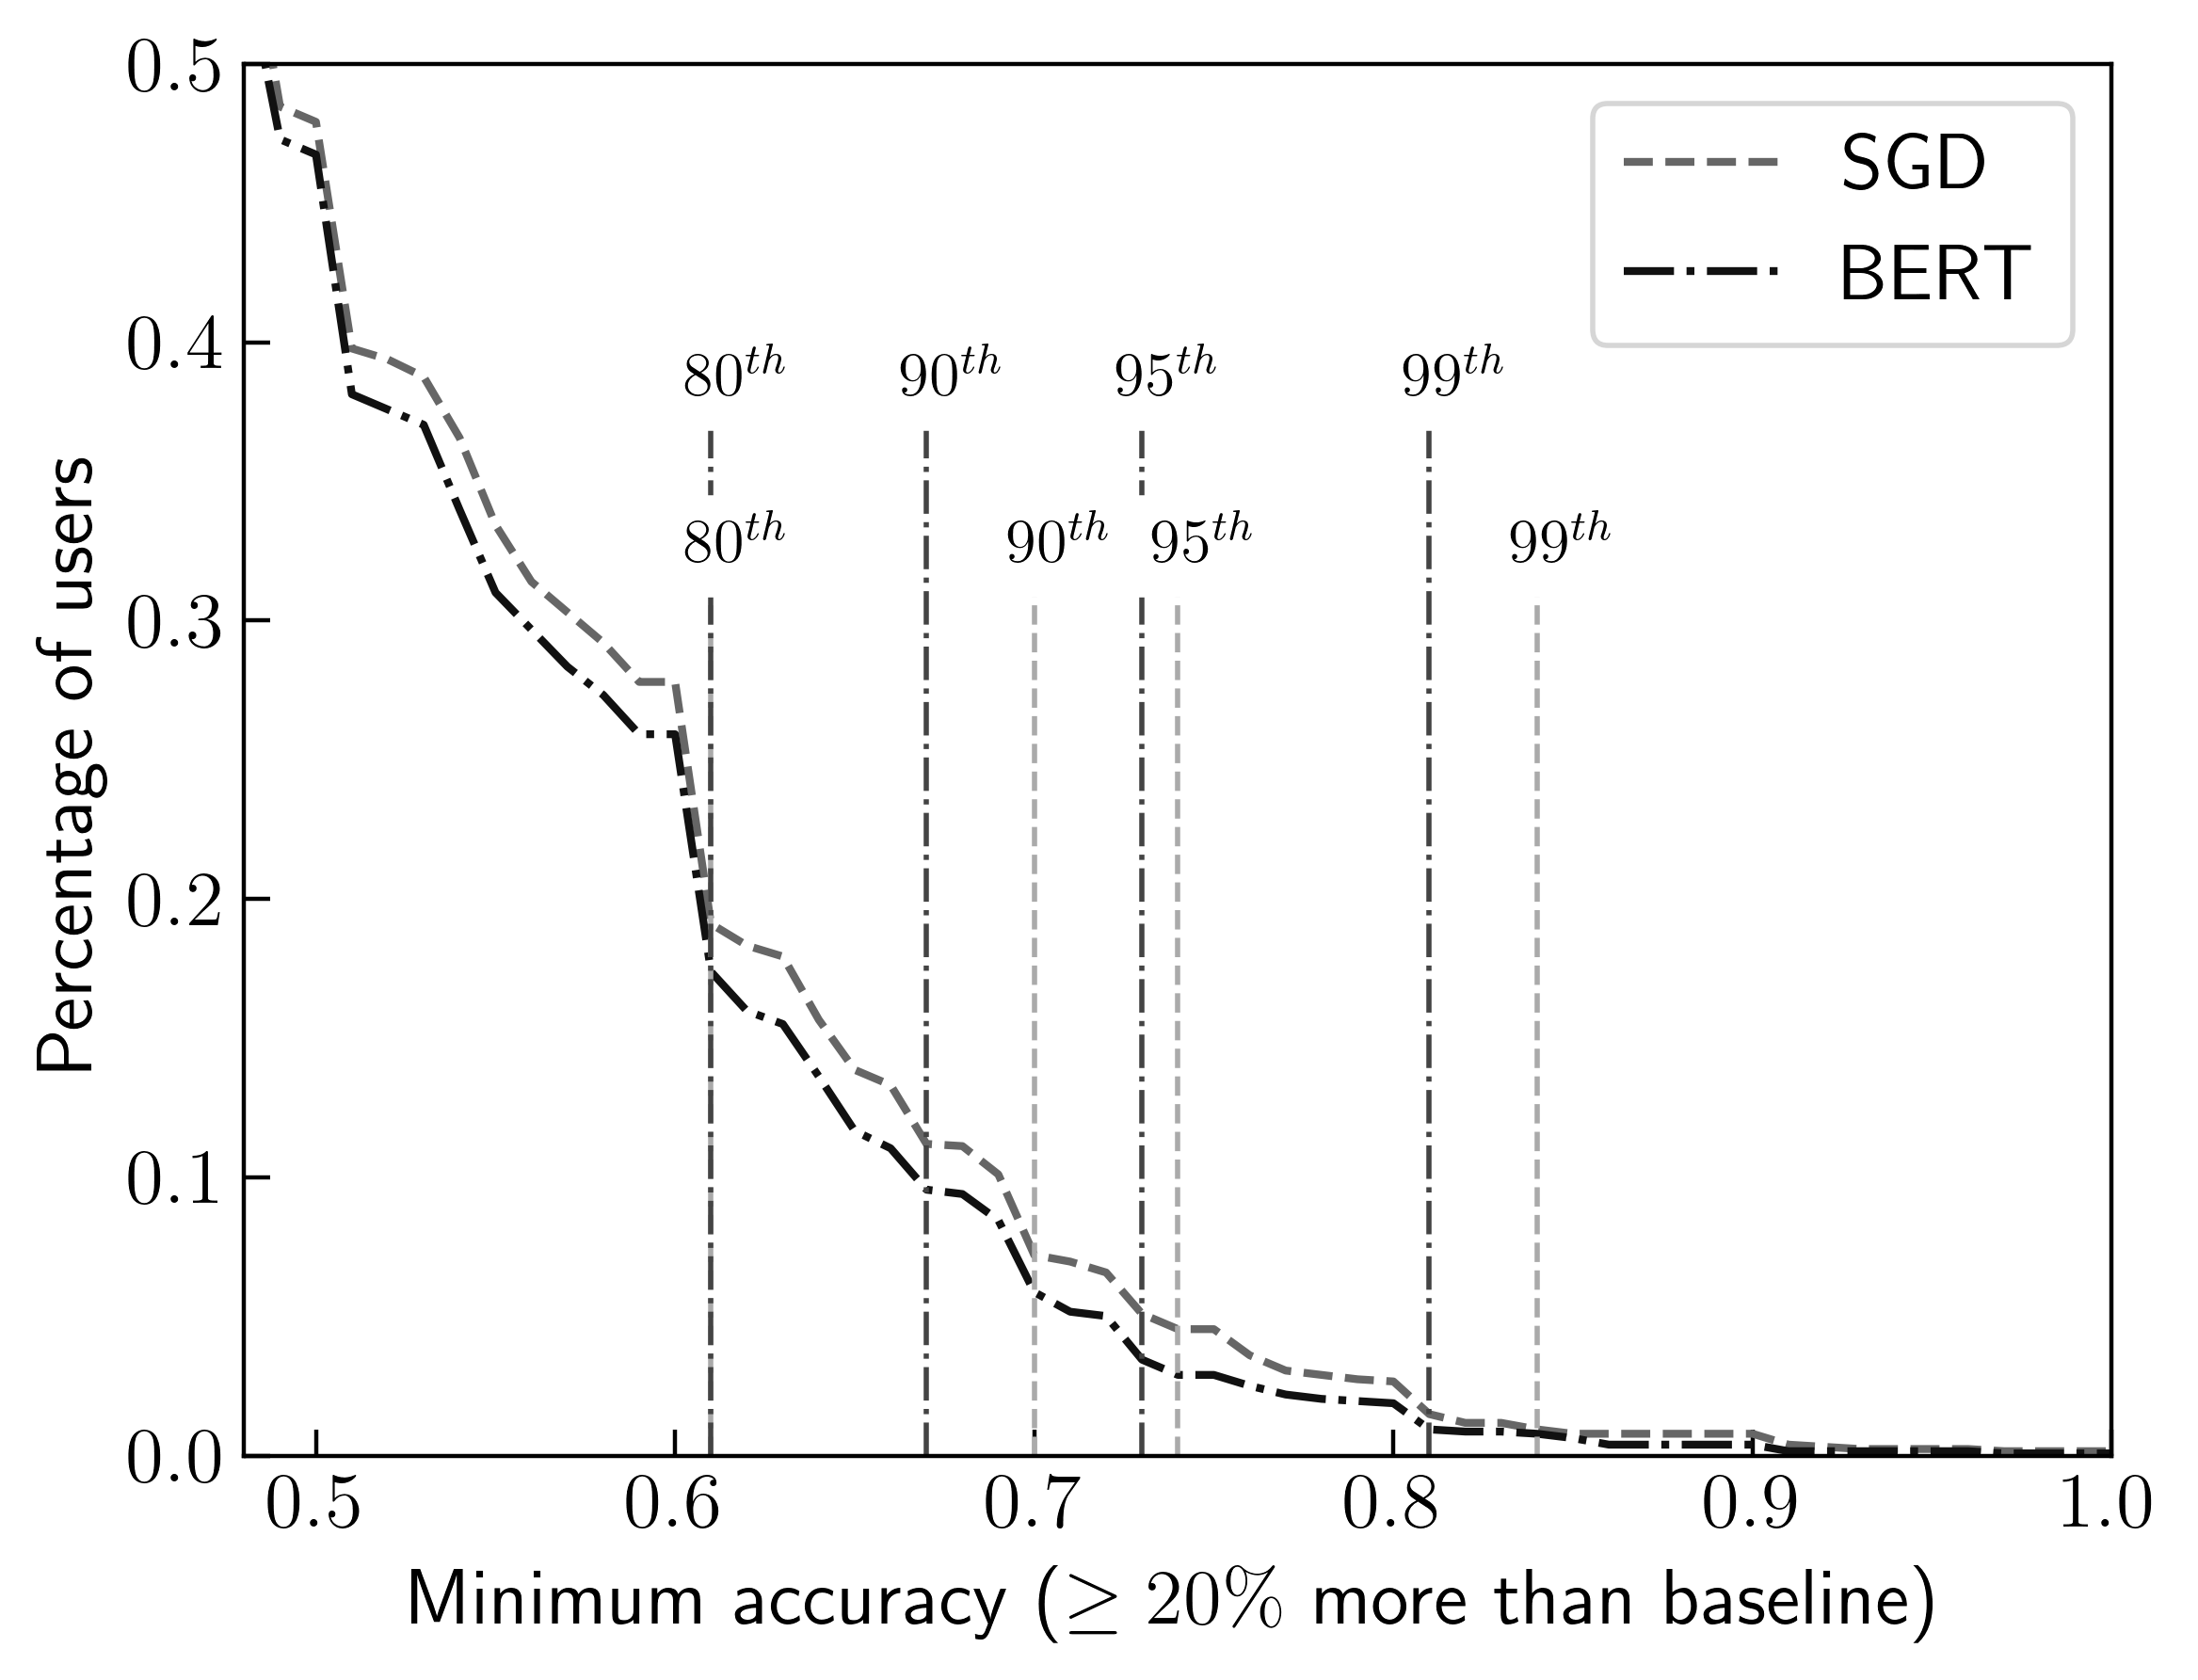
\includegraphics[width=0.7\textwidth]{figures/06_results/02_pu/03_complex/eng_6.png}
    \caption{Example of percentile selection method for English, 6-class sample.}
    \label{fig:Res_PU_PctsExample}
\end{figure}

\paragraph{Six Rating Classes}

The baseline and accompanying trained model accuracies for each user and for each of the 6-class samples can be seen in Figures \ref{fig:Res_PU_ScatterEng} and \ref{fig:Res_PU_ScatterMul}. These plots elucidate the differences between the predictions made by the trained and baseline models.

Pearson correlation coefficients are also provided in Table \ref{tab:Res_PU_Corrs} to describe the relationship between the aforementioned models' results. Each of the provided coefficients indicates a moderate correlation between the models' accuracies, with the SGD results being more strongly correlated to those of the baselines. The multilingual models are also more strongly correlated to their respective baselines than the English models.

\begin{figure}[ht]
    \centering
    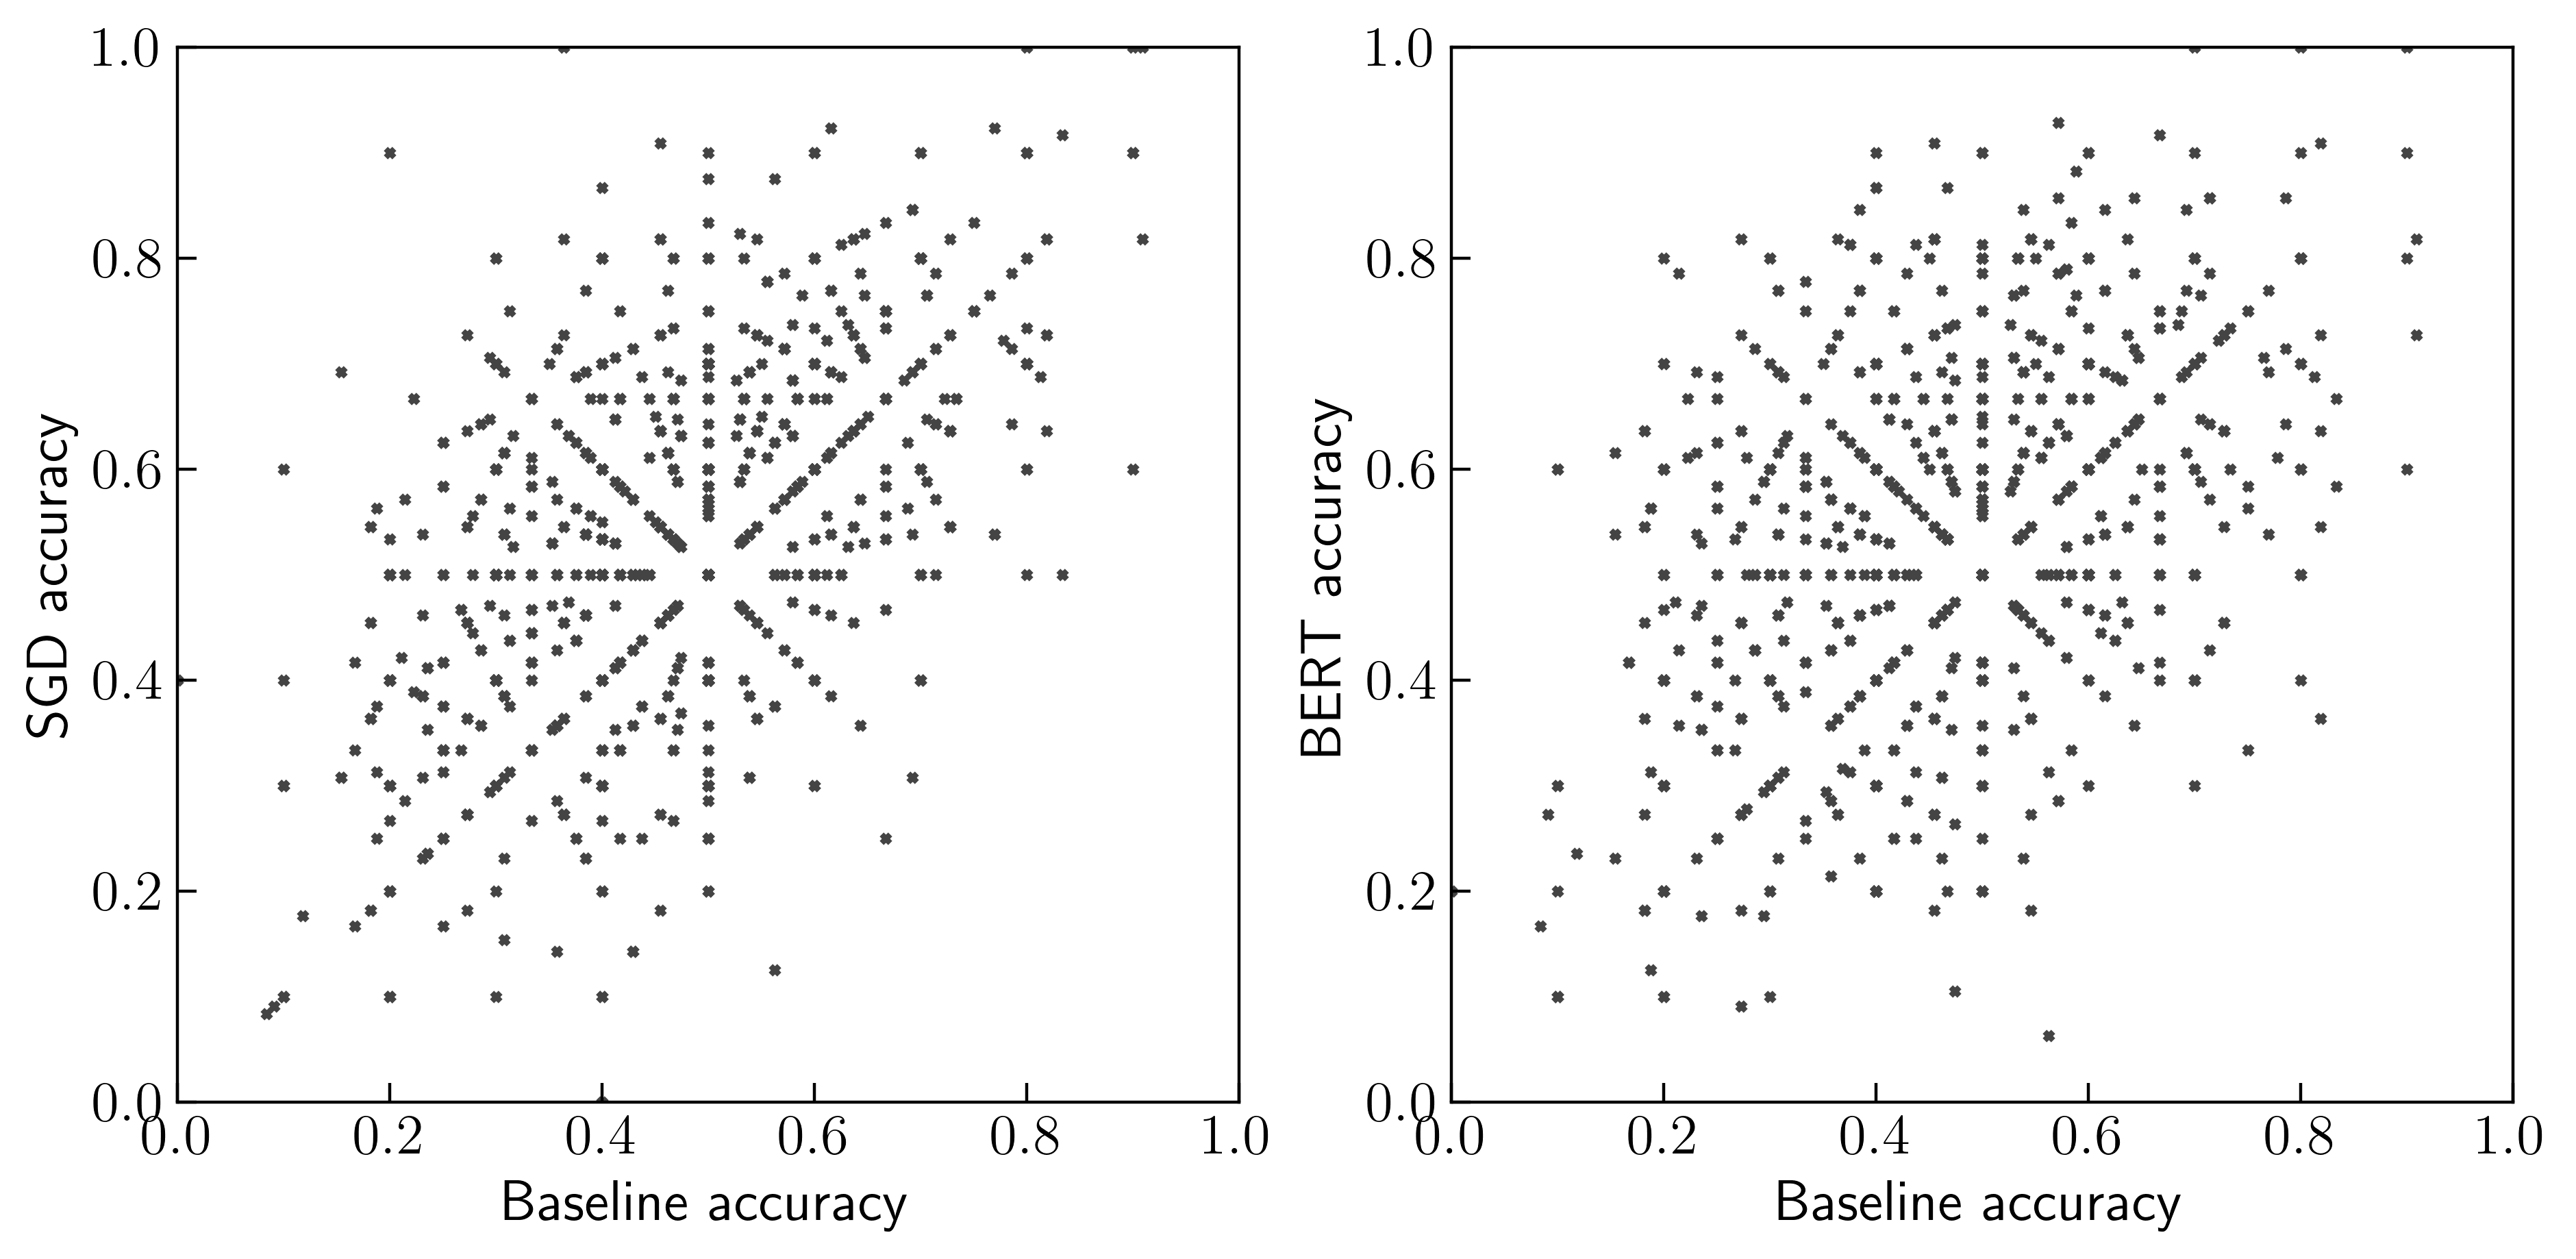
\includegraphics[width=0.9\textwidth]{figures/06_results/02_pu/04_scatter/eng_6.png}
    \caption{Comparison of model and baseline user accuracies for English, 6-class sample.}
    \label{fig:Res_PU_ScatterEng}
\end{figure}

\begin{figure}[ht]
    \centering
    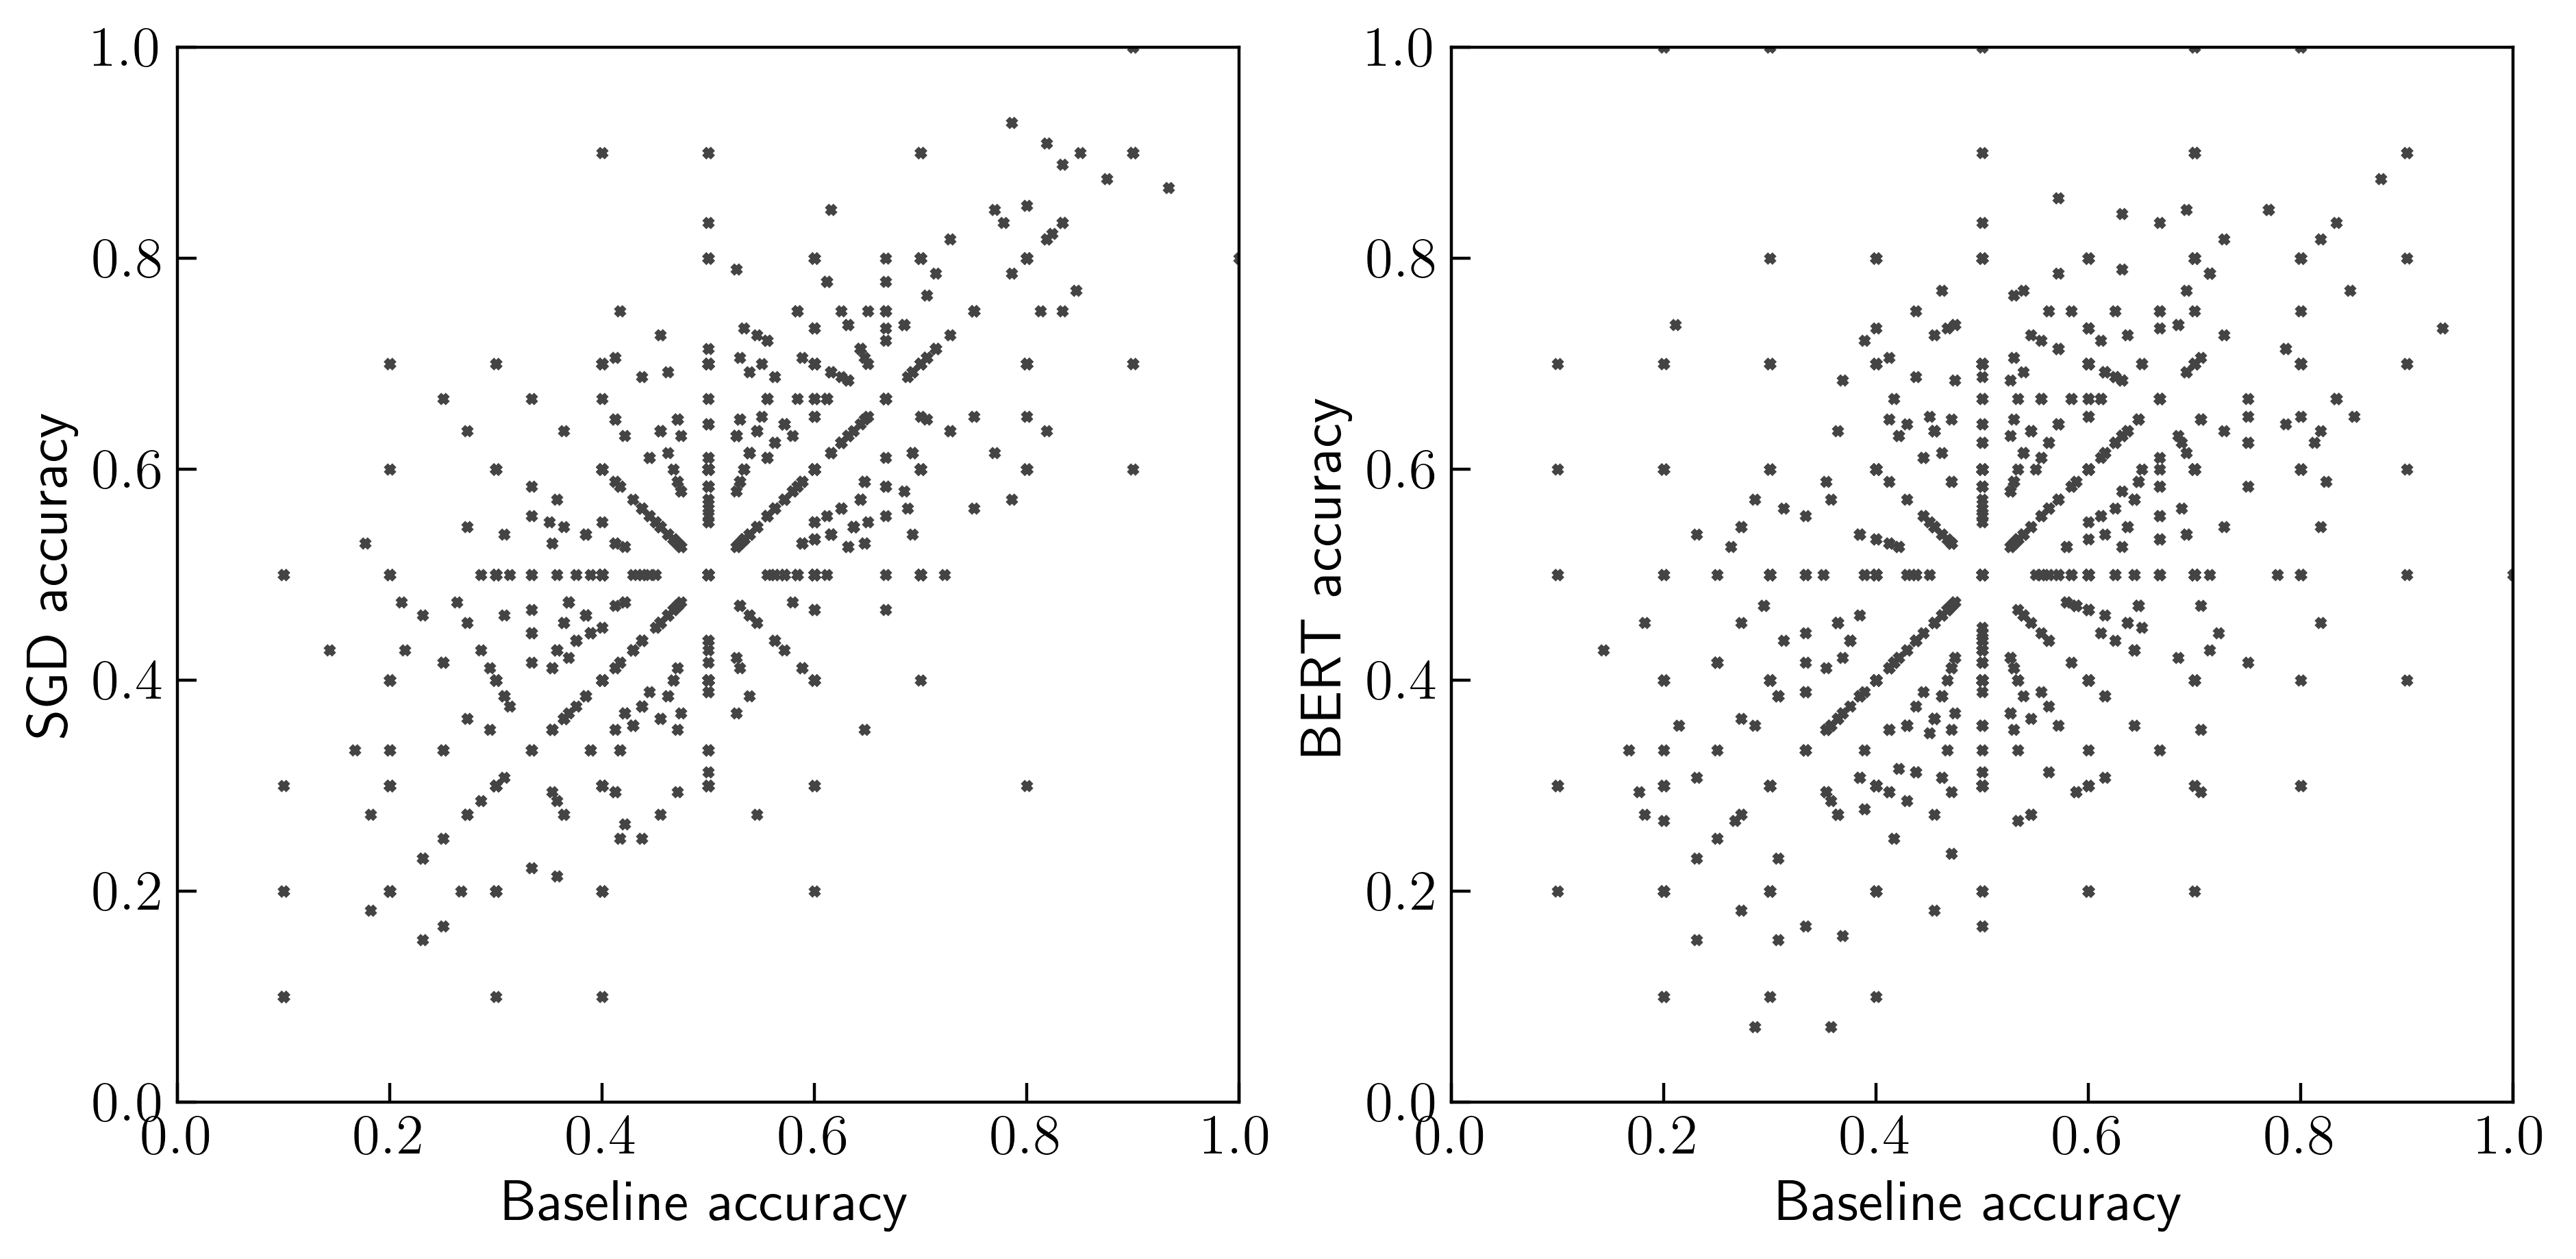
\includegraphics[width=0.9\textwidth]{figures/06_results/02_pu/04_scatter/any_6.png}
    \caption{Comparison of model and baseline user accuracies for multilingual, 6-class sample.}
    \label{fig:Res_PU_ScatterMul}
\end{figure}

\begin{table}[ht]
    \centering
    \begin{tabular}{l l | c}
        \toprule
        \textbf{Language}&\textbf{Model}&\textbf{Coefficient}\\\midrule
        English&SGD&$0.547$\\
        English&BERT&$0.42$\\\midrule
        Multilingual&SGD&$0.686$\\
        Multilingual&BERT&$0.483$\\
        \bottomrule
    \end{tabular}
    \caption{Pearson correlation coefficients between baseline and model accuracies for 6-class samples.}
    \label{tab:Res_PU_Corrs}
\end{table}

These scatter plots, in combination with the correlation coefficients, indicate that, although the results of the baseline and trained models tend to be fairly similar, there is a myriad of users for whom the trained models make predictions that are a good deal more accurate than the baseline, for each combination of sample and model. It should also be noted, however, that there are plenty of users for whom the opposite effect occurs.

The minimum user accuracies required to be in the 80\textsuperscript{th}, 90\textsuperscript{th}, 95\textsuperscript{th} and 99\textsuperscript{th} percentiles, for the 6-class samples, broken down by language and model, can be seen in Table \ref{tab:Res_PU_Pcts6}. Accuracy values are provided for various `percentage above baseline' (PAB) selection criteria - with a PAB of 0\% being provided as a new and alternative form of baseline.

\begin{table}[ht]
    \centering
    \begin{tabular}{l | c | c c c c | c c c c}
        \toprule
        \multirow{2}{*}{\textbf{Language}}&\multirow{2}{*}{\textbf{PAB}}&\multicolumn{4}{c}{\textbf{SGD}}&\multicolumn{4}{|c}{\textbf{BERT}}\\
        &&\textbf{$80^{th}$} & \textbf{$90^{th}$} & \textbf{$95^{th}$} & \textbf{$99^{th}$} & \textbf{$80^{th}$} & \textbf{$90^{th}$} & \textbf{$95^{th}$} & \textbf{$99^{th}$}\\\midrule
        English&$0\%$&$0.58$&$0.64$&$0.70$&$0.81$&$0.55$&$0.61$&$0.67$&$0.81$\\
        English&$10\%$&$0.61$&$0.67$&$0.72$&$0.82$&$0.59$&$0.65$&$0.70$&$0.81$\\
        English&$20\%$&$0.61$&$0.70$&$0.74$&$0.84$&$0.61$&$0.67$&$0.73$&$0.81$\\
        English&$30\%$&$0.64$&$0.70$&$0.76$&$0.85$&$0.62$&$0.70$&$0.74$&$0.84$\\
        English&$40\%$&$0.65$&$0.70$&$0.77$&$0.87$&$0.64$&$0.70$&$0.76$&$0.85$\\\midrule
        Multilingual&$0\%$&$0.61$&$0.69$&$0.70$&$0.82$&$0.61$&$0.63$&$0.70$&$0.81$\\
        Multilingual&$10\%$&$0.62$&$0.70$&$0.74$&$0.85$&$0.61$&$0.67$&$0.70$&$0.81$\\
        Multilingual&$20\%$&$0.63$&$0.70$&$0.76$&$0.85$&$0.61$&$0.70$&$0.73$&$0.84$\\
        Multilingual&$30\%$&$0.65$&$0.70$&$0.78$&$0.88$&$0.62$&$0.70$&$0.74$&$0.85$\\
        Multilingual&$40\%$&$0.65$&$0.70$&$0.78$&$0.88$&$0.63$&$0.70$&$0.74$&$0.85$\\
        \bottomrule
    \end{tabular}
    \caption{Minimum accuracies required to be included by various percentile selection methods for 6-class samples.}
    \label{tab:Res_PU_Pcts6}
\end{table}

A point worth noting is that a larger PAB might not necessarily lead to more representative users being determined. For example, a user with an SGD/BERT accuracy of 100\% and a baseline accuracy of 75\% might be considered a representative user; however, given a PAB of 40\% the minimum included SGD/BERT accuracy would be 105\% which is, of course, impossible to achieve. Conversely, a user with an SGD/BERT accuracy of 100\% but a baseline accuracy of 90\% might not be considered particularly representative due to their high baseline accuracy; however, a smaller PAB, such as 10\%, would lead to their inclusion as a representative user. For the sake of simplicity, a PAB of 20\% will be considered a suitable middle ground.

For both the English and multilingual samples, the SGD classifier consistently required slightly higher accuracies than the BERT classifier for a given user to be included in each of the specified percentiles. For the multilingual sample, somewhat surprisingly, the required accuracies were slightly higher than those required by the English model.

The accuracies required for a user to be included in the 80\textsuperscript{th}, 90\textsuperscript{th} and, occasionally, the 95\textsuperscript{th} percentiles, are fairly low, regardless of the PAB, so they should probably not be considered suitable cut-off points when determining which users are representative. The accuracies required for a user to be included in the 99\textsuperscript{th} percentile, however, are sufficiently high and so it could be probably considered a suitable cut-off point.

The accuracies required for a user to be included in the 99\textsuperscript{th} percentile do not increase by a particularly large amount when the PAB is increased which could be an indication that the potential drawbacks regarding larger and smaller PABs may not be as impactful as was initially implied.

\subsection{Discussion}

The approach used to determine potentially representative users was, in essence, an extension of the work done to predict review polarity. The high accuracy of the models trained to predict polarity using nothing but the review text was a clear indication that there were particular features present within the written reviews that the machine learning models could identify and utilise to make accurate predictions.

The representative users approach simply expanded the binary classification problem of polarity prediction into a multinomial classification problem involving the prediction of average game ratings. The limitations involved with this approach, as well as the various assumptions that were made, have already been detailed in previous sections of this report In summary, a significant portion of the training data was of poor quality and, as a result, the input text did not always `agree' with the desired output class. As was the case with polarity prediction, difficulties arose due to the distribution of output classes being highly imbalanced.

When evaluated based on their overall accuracies, the models trained on the 6-class samples, particularly the English-language ones, performed a good deal better than the baseline classifiers, despite all of the potential data problems that had been discussed. These results were quite promising as they indicated that the trained models were still capable of identifying predictive features in the review data, irrespective of the `noise' that was present.

The models trained on the 3-class samples did not perform any better than their baselines, although, due to the extremely imbalanced nature of the samples in question, this was not particularly surprising.

By analysing the results of the 6-class models on a per-user basis, the users whose written reviews most accurately predict the overall rating of the game being reviewed, at least according to the model, can be determined. Users whose trained model accuracies are not significantly higher than their baseline accuracies can also be excluded.

The users whose trained model accuracies were in the 99\textsuperscript{th} percentile were considered to be suitably representative. The SGD models required a higher user accuracy than the BERT models and thus appeared to be performing better. However, the multilingual models also required a higher user accuracy than the English models which, given the former's poorer overall performance, might indicate that the required user accuracy could potentially be a misleading or incomplete metric.

Nonetheless, given that both the overall accuracies of certain 6-class models were higher than their respective baselines, and that, on a per-user basis, even when controlling for the performance of baselines, a considerable proportion of users had their reviews predicted accurately enough to be considered representative, this approach appears to show some potential and may be worthy of further investigation.

A number of possible alterations to the methods employed when tackling this problem spring to mind. As was already discussed when evaluating the polarity prediction results, the size of the dataset samples could be substantially increased in order to improve the quality of the BERT models. The selective sampling of reviews based on their word count, a technique that was also applied to the prediction of review polarities, might be relevant to this problem, too. Reviews already considered `helpful' by the Steam community, ie those with a certain number of votes, could be exclusively sampled as a means of reducing the presence of poor quality data being used to train the models. Finally, the dataset could be sampled in a more balanced manner, with additional reviews being included for games with `mixed' or `negative' ratings.
